\chapter{Quench Recognition Problem (QRP)}
\label{chp:qrp}
This chapter is dedicated to the solution of \qrp, which we introduced in \Cref{chp:problem}, in this chapter we will:
\begin{itemize}
	\item Give a rapid overview of the problem, analyzing the results obtained from
	      preprocessing,
	\item Talk about the models used, and the results obtained for each model,
	\item Select the 'best' possible model.
\end{itemize}

\section{Problem description}
As was introduced in the previous chapter our dataset consists of four tables of $279$ samples
each, divided between 'quench' ($1$) and 'non-quench' ($0$) events, the distribution is not exactly balanced: $192$ quench events and $87$ non-quench events; since the imbalance is not extreme we didn't take explicit action against it.

\section{Data preprocessing}
\label{sec:qrp-preprocessing}
Before working on the actual models we analyzed:
\begin{itemize}
	\item the cross-correlations between the harmonics, which aims to identify repeated
	      information within the dataset;
	\item the cross-correlation between the harmonics and the labels, which indicates how
	      well the harmonics of the dataset are capable of explaining the expected results;
	\item the box plot of the attributes, which is visualizes the variability of the harmonics,
	      giving us a powerful tool to understand which ones are more relevant to the
	      computation, and
	\item the distribution of data after dimensionality reduction via principal component
	      analysis (\pca), which is meant to give a good idea of how the data are distributed
	      and hints to which are the better attributes to solve the problem.
\end{itemize}
In the following, the vector containing the information about the correlation with the labels has
been plotted after a normalization step, which was done by training an instance of the MinMaxScaler
class from scikit-learn. While this procedure doesn't change the intensity of the correlation
between the harmonic and the label it makes the plots more readable and easier to interpret, the normalized samples are scaled using \Cref{eq:normalization} \cite{Nishok2024}.
\begin{equation}
	\label{eq:normalization}
	X_\text{scaled} = \frac{X - X_\text{min}}{X_\text{max} - X_\text{min}}
\end{equation}
Where $X$ is a sample in the vector that is being scaled.

We will be covering the results of preprocessing in four different sections, each dedicated to one
attribute.

\subsubsection{\an}
\Cref{fig:an-corr} among the harmonics. Independently of the sign, the matrix evidently contains a
pattern, hinting to the fact that many harmonics contain repeated information, (e.g., \an[1] provides
the same information as \an[3], \an[5], \an[7]), \ldots By analyzing the figure we can reach the
following conclusions:
\begin{itemize}
	\item Its strong geometry implies that doing feature extraction is going to be complex (as
	      we will see in the following sections it's basically a shared characteristic for
	      almost all the attributes), due to the necessity of finding a mix of harmonics that has a high correlation with the label, while having a low correlation among themselves.
	\item All the odd harmonics are strongly correlated with each other (with the sole exception
	      of \an[15]),
	\item \an[2] is strongly correlated with its odd multiples (i.e., \an[6], \an[10], \an[14]),
	\item \an[4] is strongly correlated with all its multiples (i.e., \an[8], \an[12]),
	\item \an[15] is the only one not correlated to any of the other harmonics.
\end{itemize}
\begin{figure}[!ht]
	\centering
	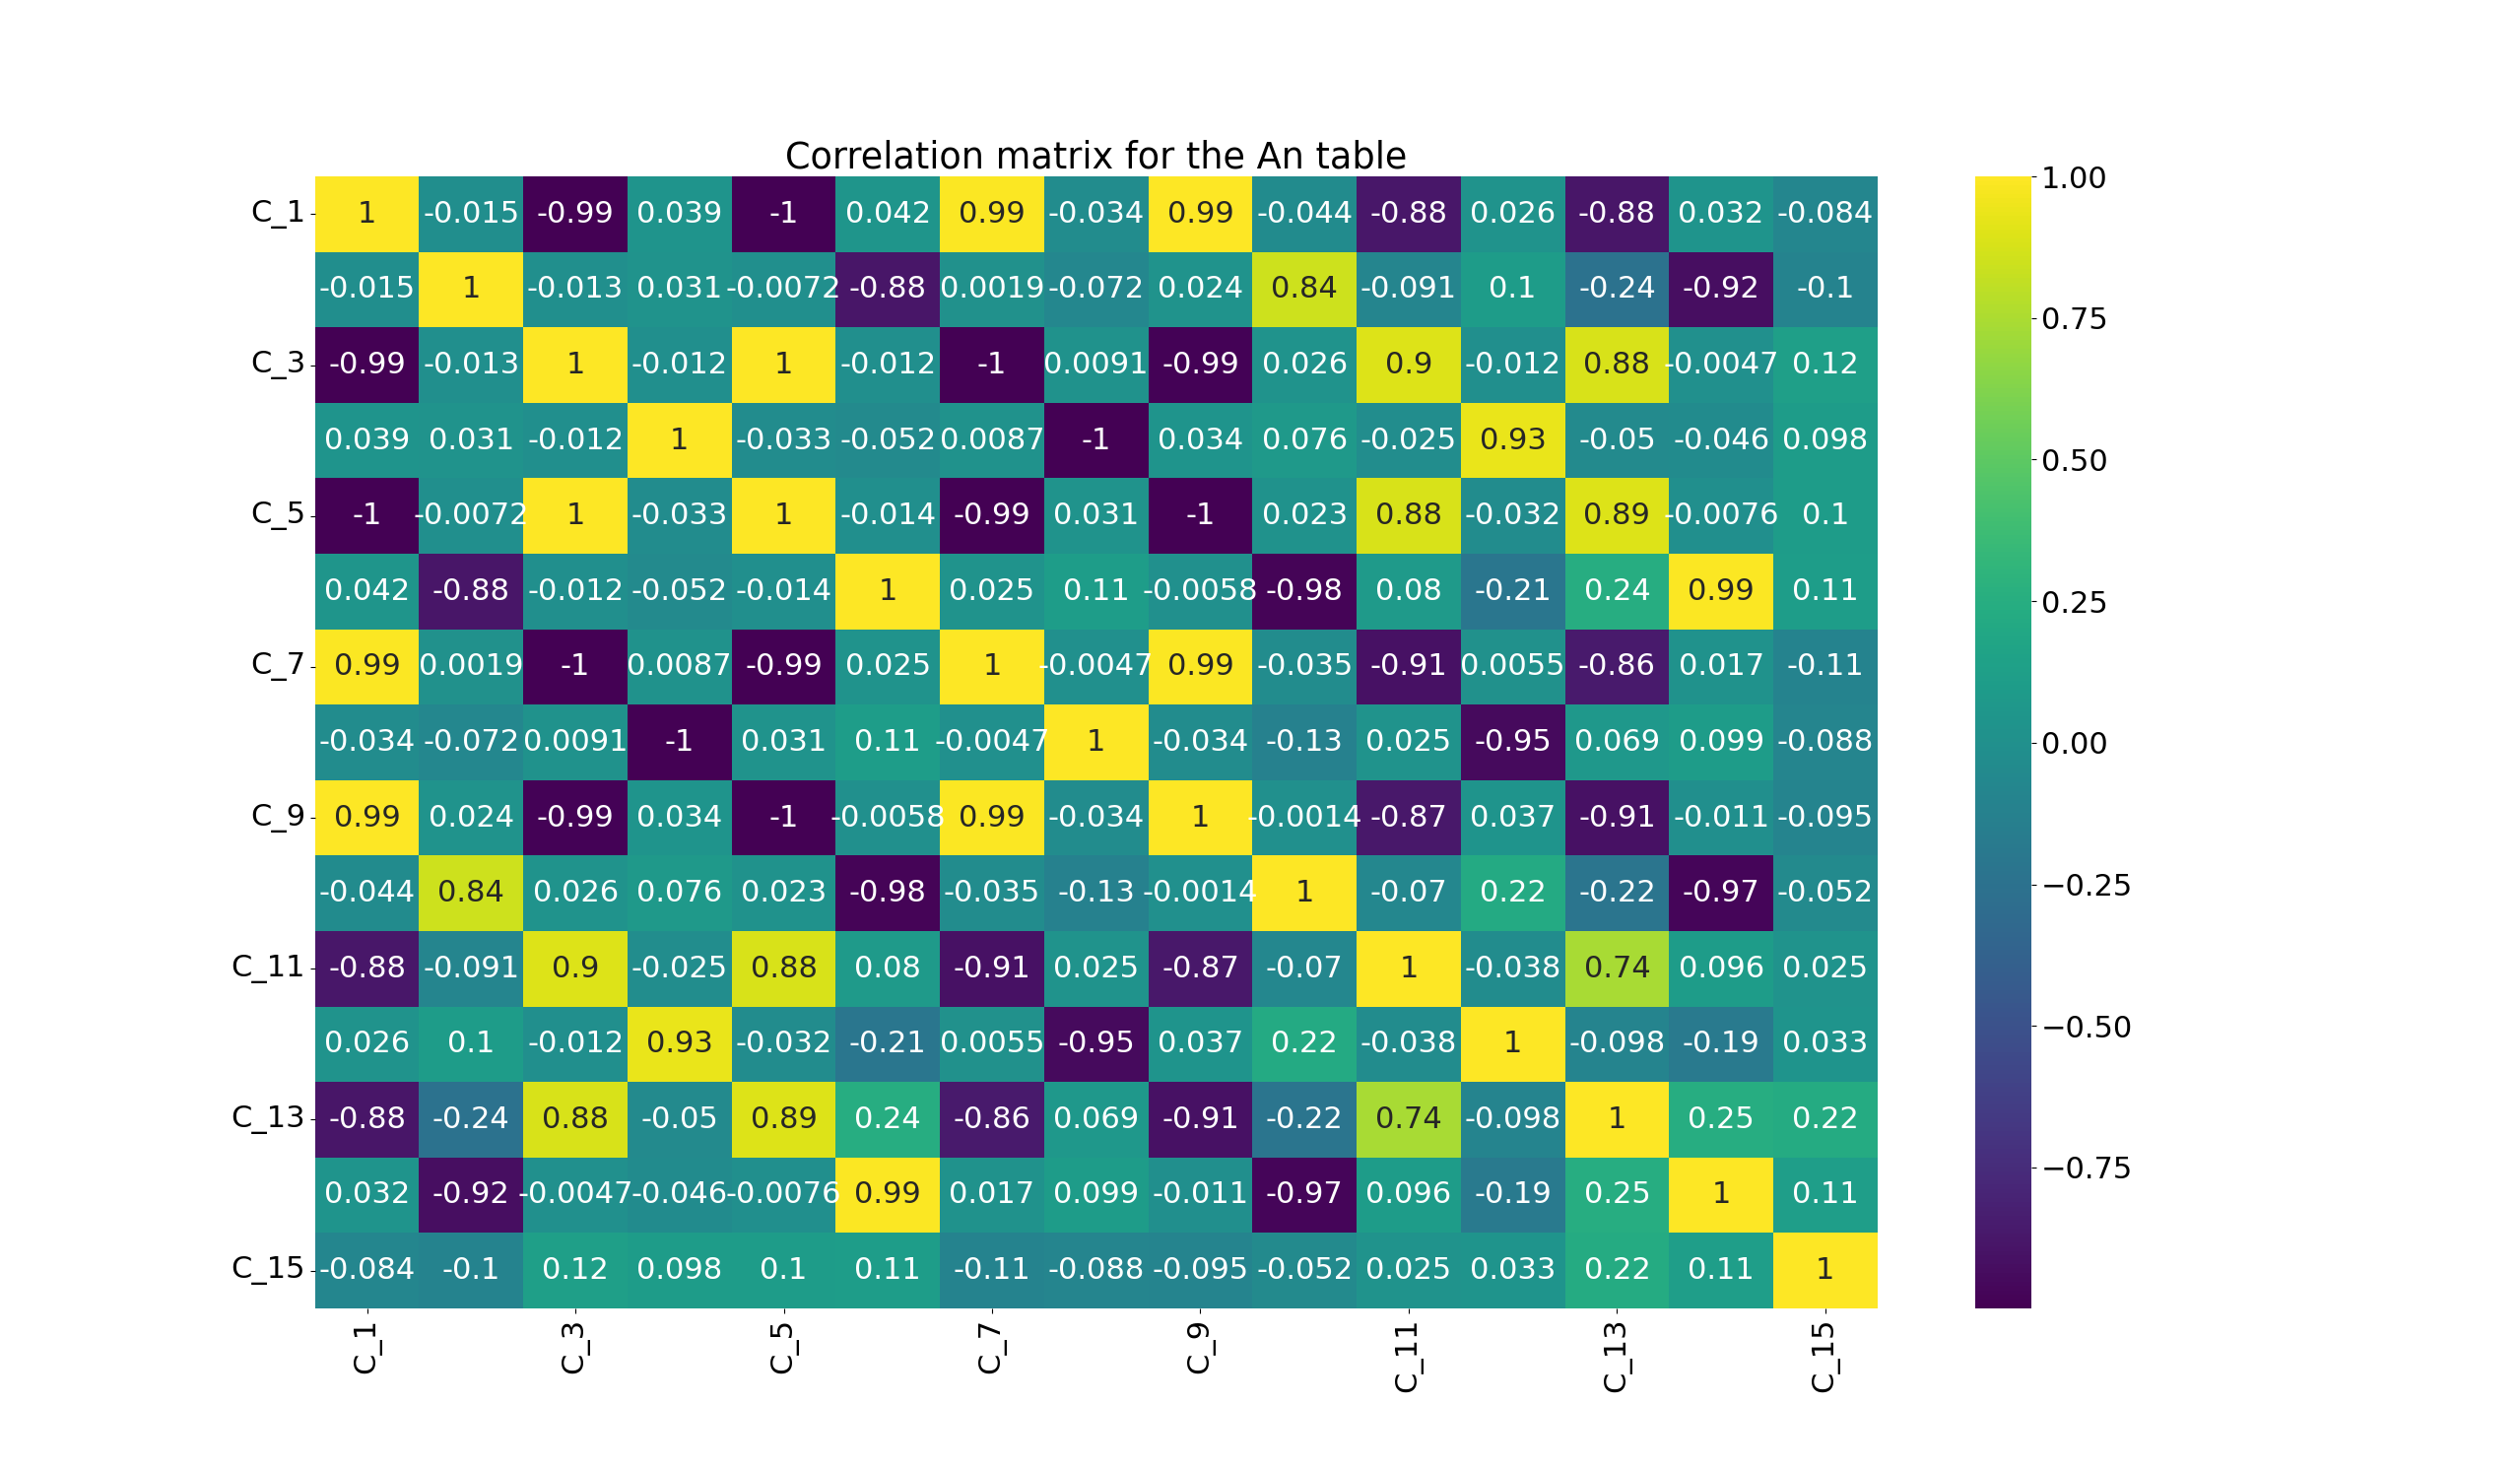
\includegraphics[width=\linewidth]{img/An_corr_matrix.png}
	\caption{The cross-correlation among the \an\ harmonics.} \label{fig:an-corr}
\end{figure}

If we consider \Cref{fig:an-lcorr}, and we pick the harmonics with the highest label correlation,
identified by a higher color intensity, we end up with the following set of features: \{\an[2],
\an[6], \an[10], \an[11], \an[12], \an[13], \an[14], \an[15]\}. This is interesting because:
\begin{enumerate}
	\item \an[2], as well as its odd multiples, can explain the results well, which is what we expect from the theory.
	\item High order harmonics are able to explain the results better than other harmonics,
	      which is not what we would have expected, since in the original analysis the value for the
	      labels was computed using primarily low-order harmonics\footnote{By low order
		      harmonics we intend the harmonics going from $1$ to $6$ circa}.
\end{enumerate}

\begin{figure}[!ht]
	\centering
	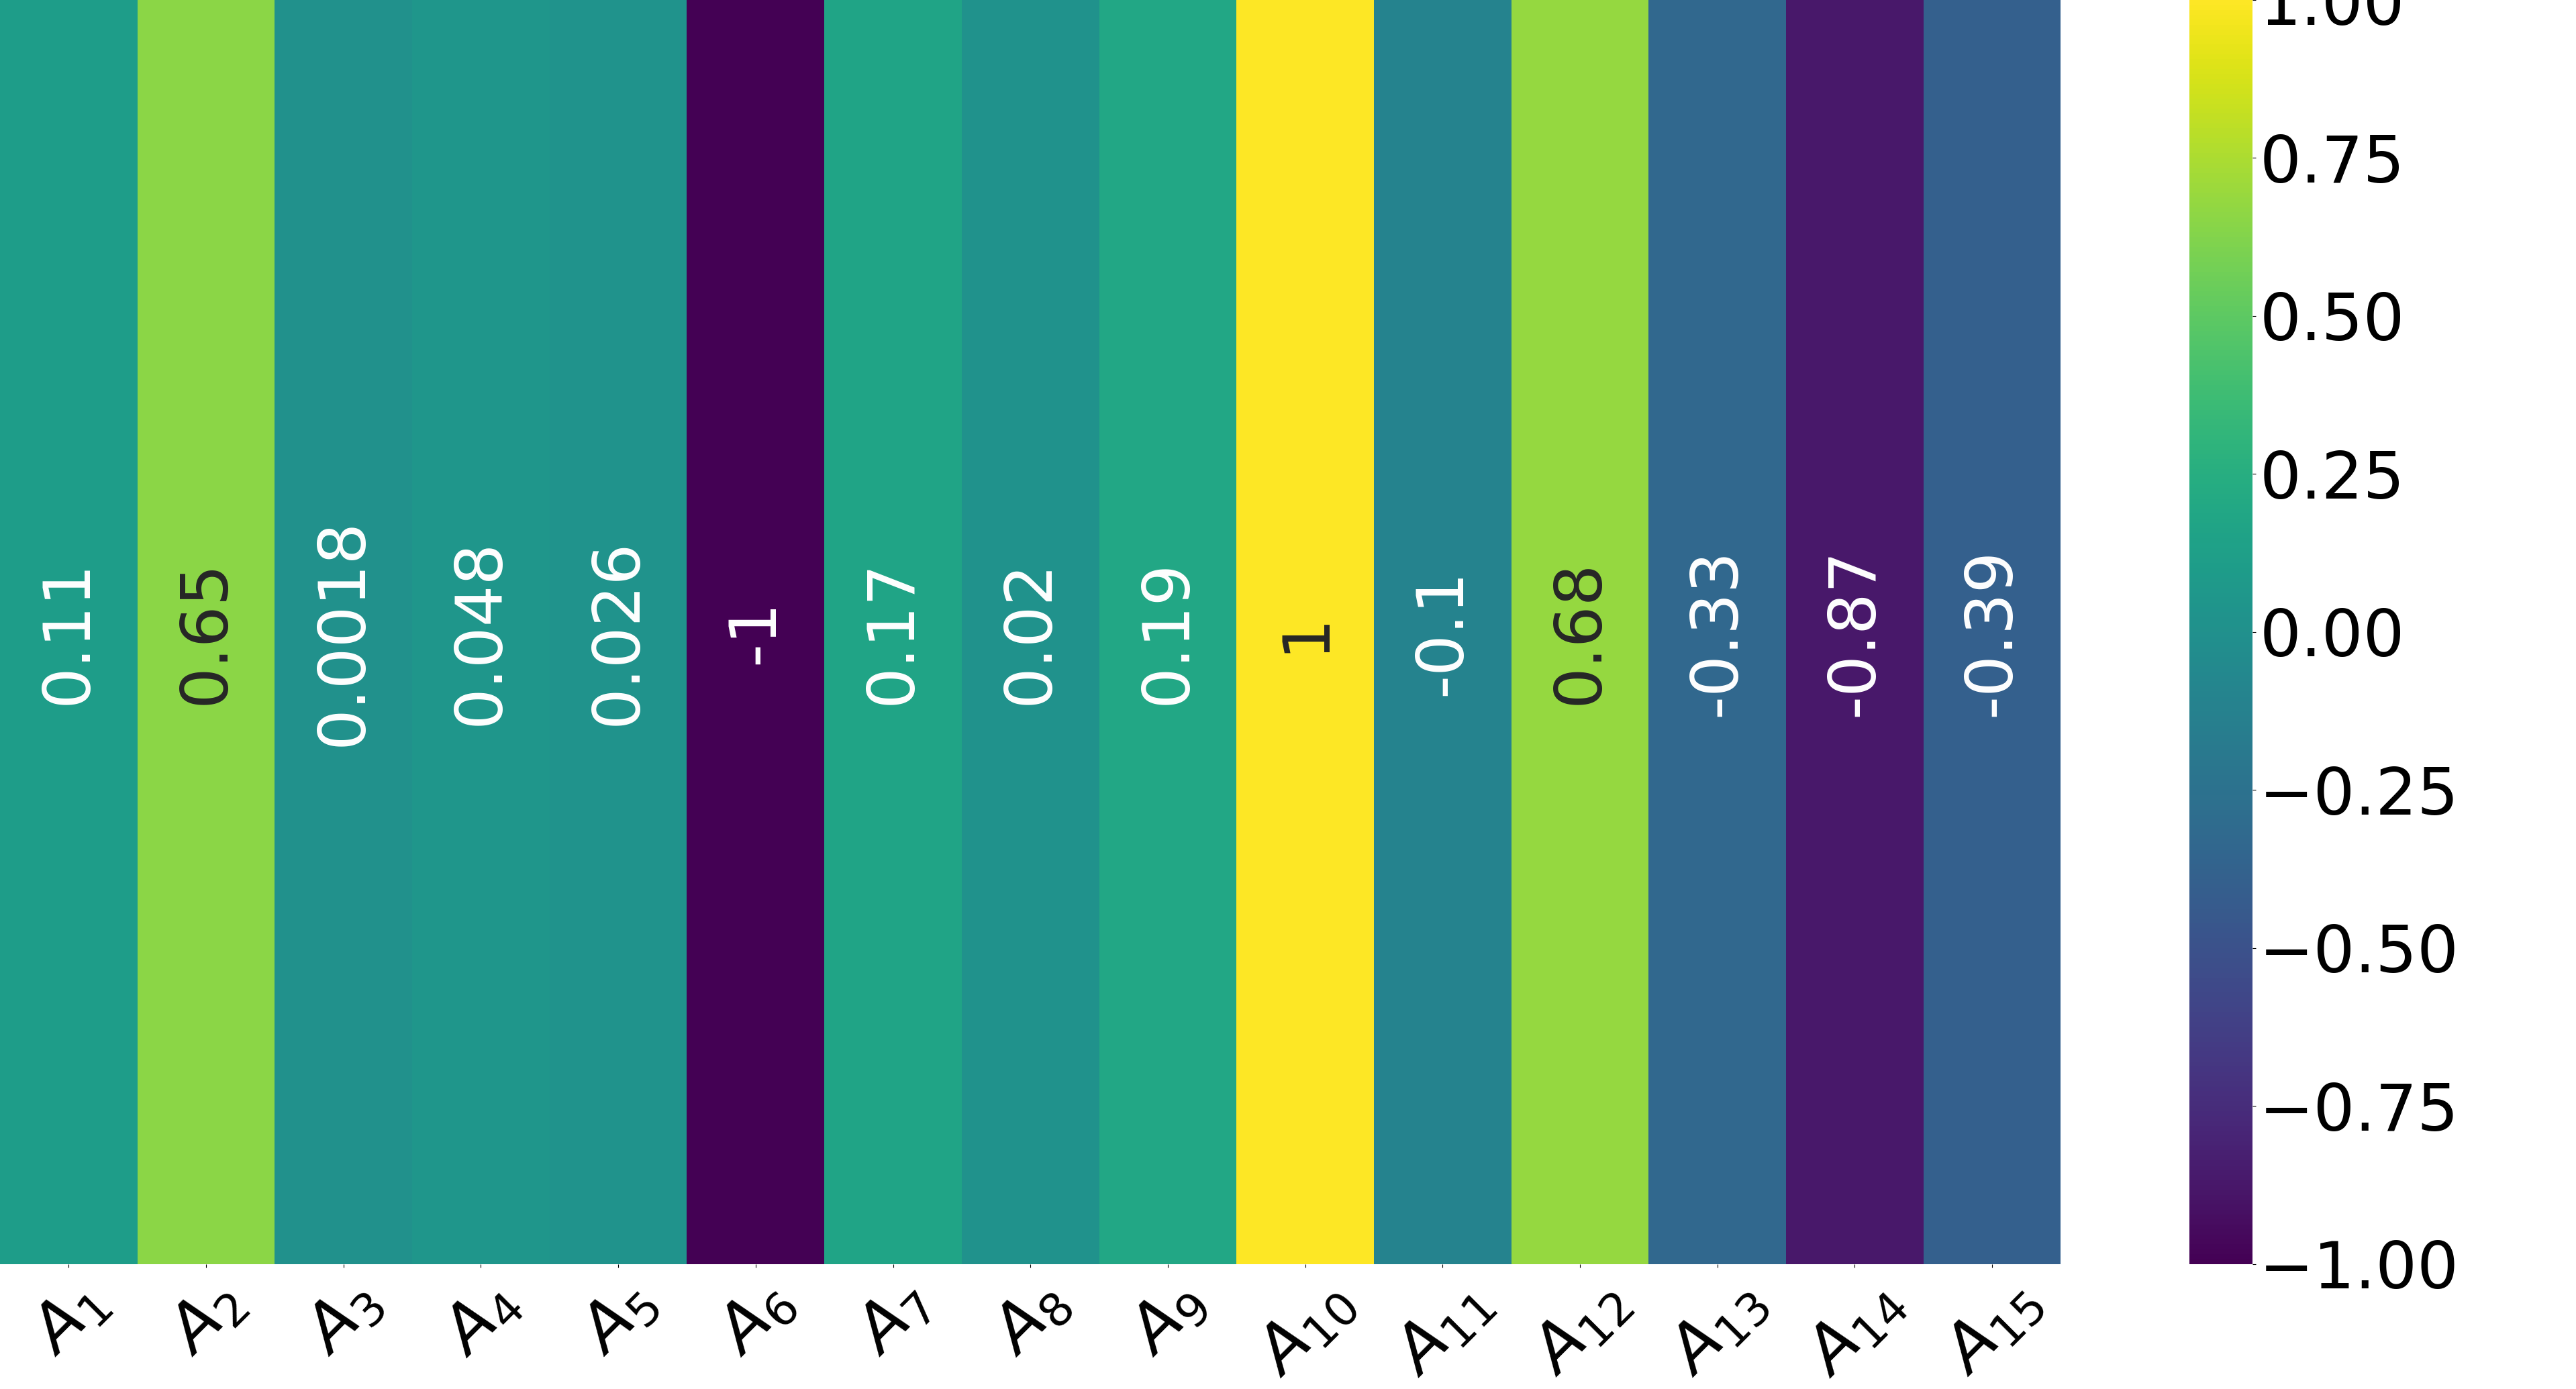
\includegraphics[width=\linewidth]{img/An_label_corr.png}
	\caption{Correlation between the harmonics and the labels for \an.} \label{fig:an-lcorr}
\end{figure}

The structure of the correlation matrix and the correlation between labels and harmonics leads us to
believe that a good-performing sub-view for \an\ should contain \an[2], or one of its high-order
odd multiples, as well as \an[15]\ and some other high-order harmonics like \an[11]\ or \an[13].

Lastly, we can visualize the distribution of samples in bidimensional space, achieved by using \pca\
dimensionality reduction.
\begin{figure}[!ht]
	\centering
	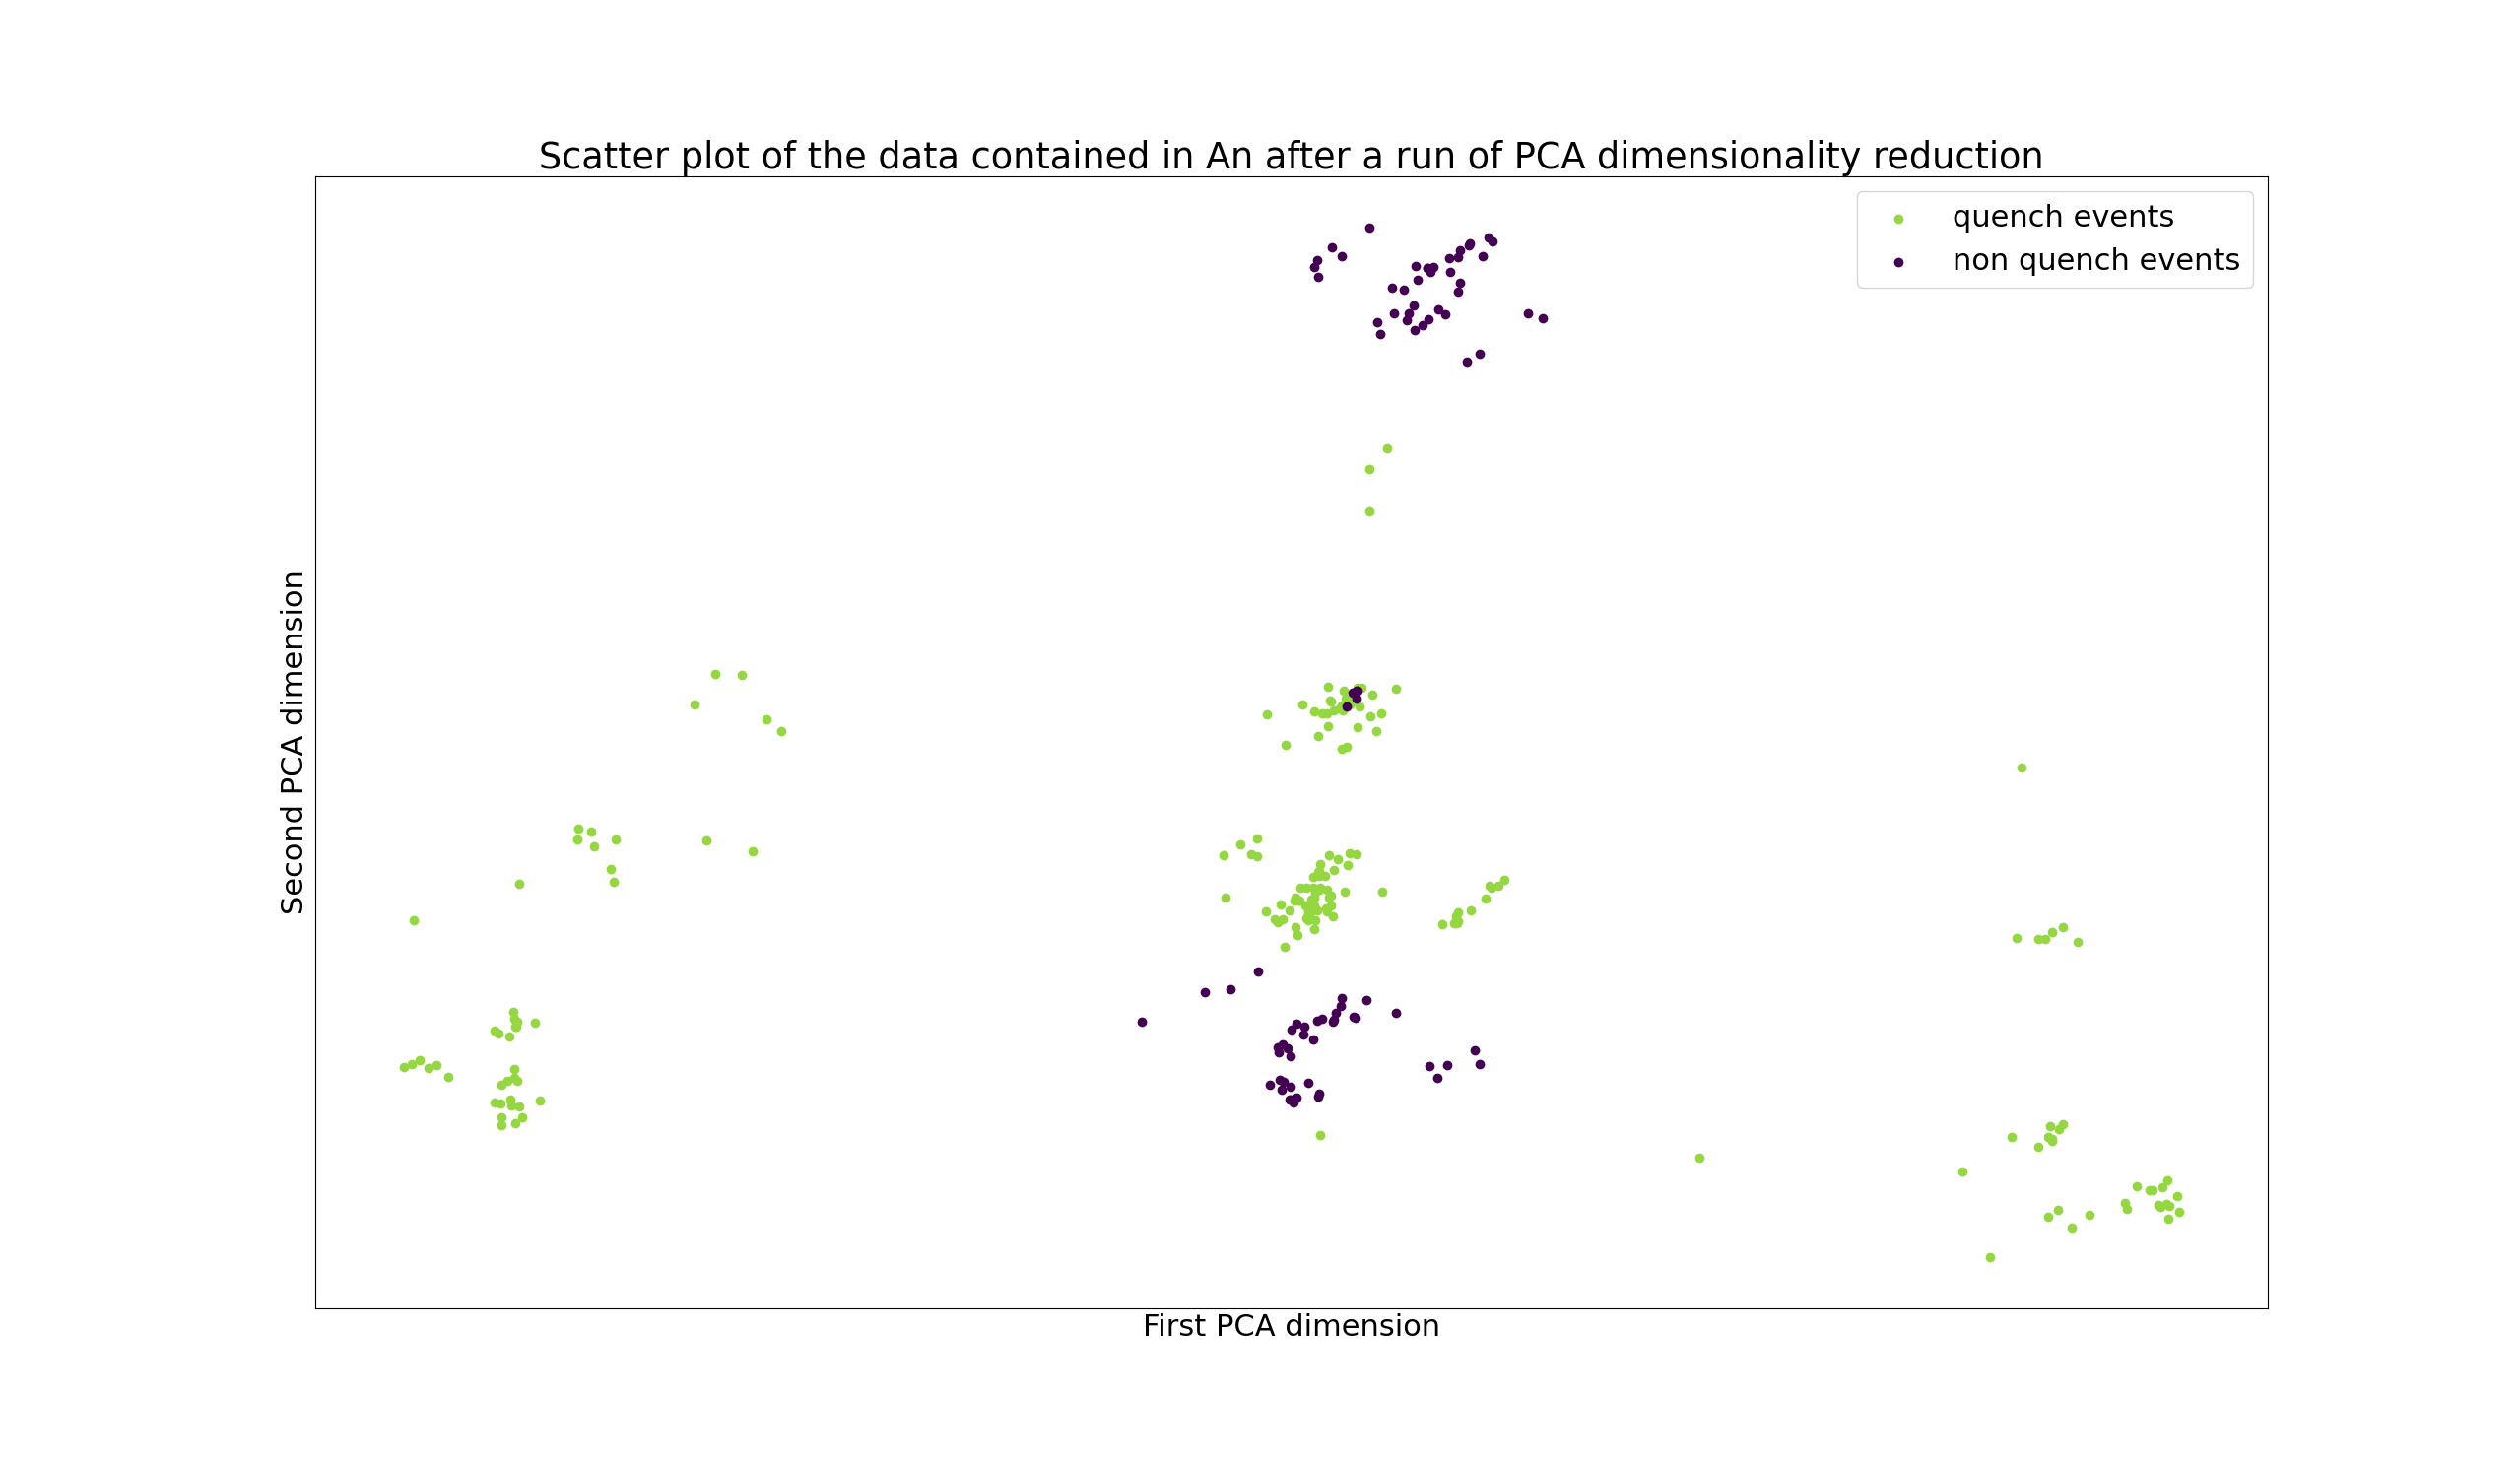
\includegraphics[width=\linewidth]{img/An_distribution.png}
	\caption{Data distribution for the \an\ table after applying \pca\ dimensionality
		reduction, moving from $15$-dimensional space to $2$-dimensional space-dimensional
		space. In the plot we highlight quench and non-quench events.} \label{fig:an-dist}
\end{figure}

As we will see in the following sections, the distribution shown in \Cref{fig:an-dist}, with its
clear-cut clusters characterized by a high level of purity, is the best distribution among the
alternatives. Having such a good distribution lead us to think that it might be the reason why
models built on \an\ and \cnmod\ (at least for \qrp) perform better than the ones built on \bn\ and
\phin.

\subsubsection{\bn}
We can use a similar procedure on the \bn\ attribute, which in most tests proved to be the
least-performing attribute. This is probably due to the poor distribution of the data, as we can see in
\Cref{fig:bn-dist}, the central cluster has a very high level of homogeneity.
\begin{figure}[!ht]
	\centering
	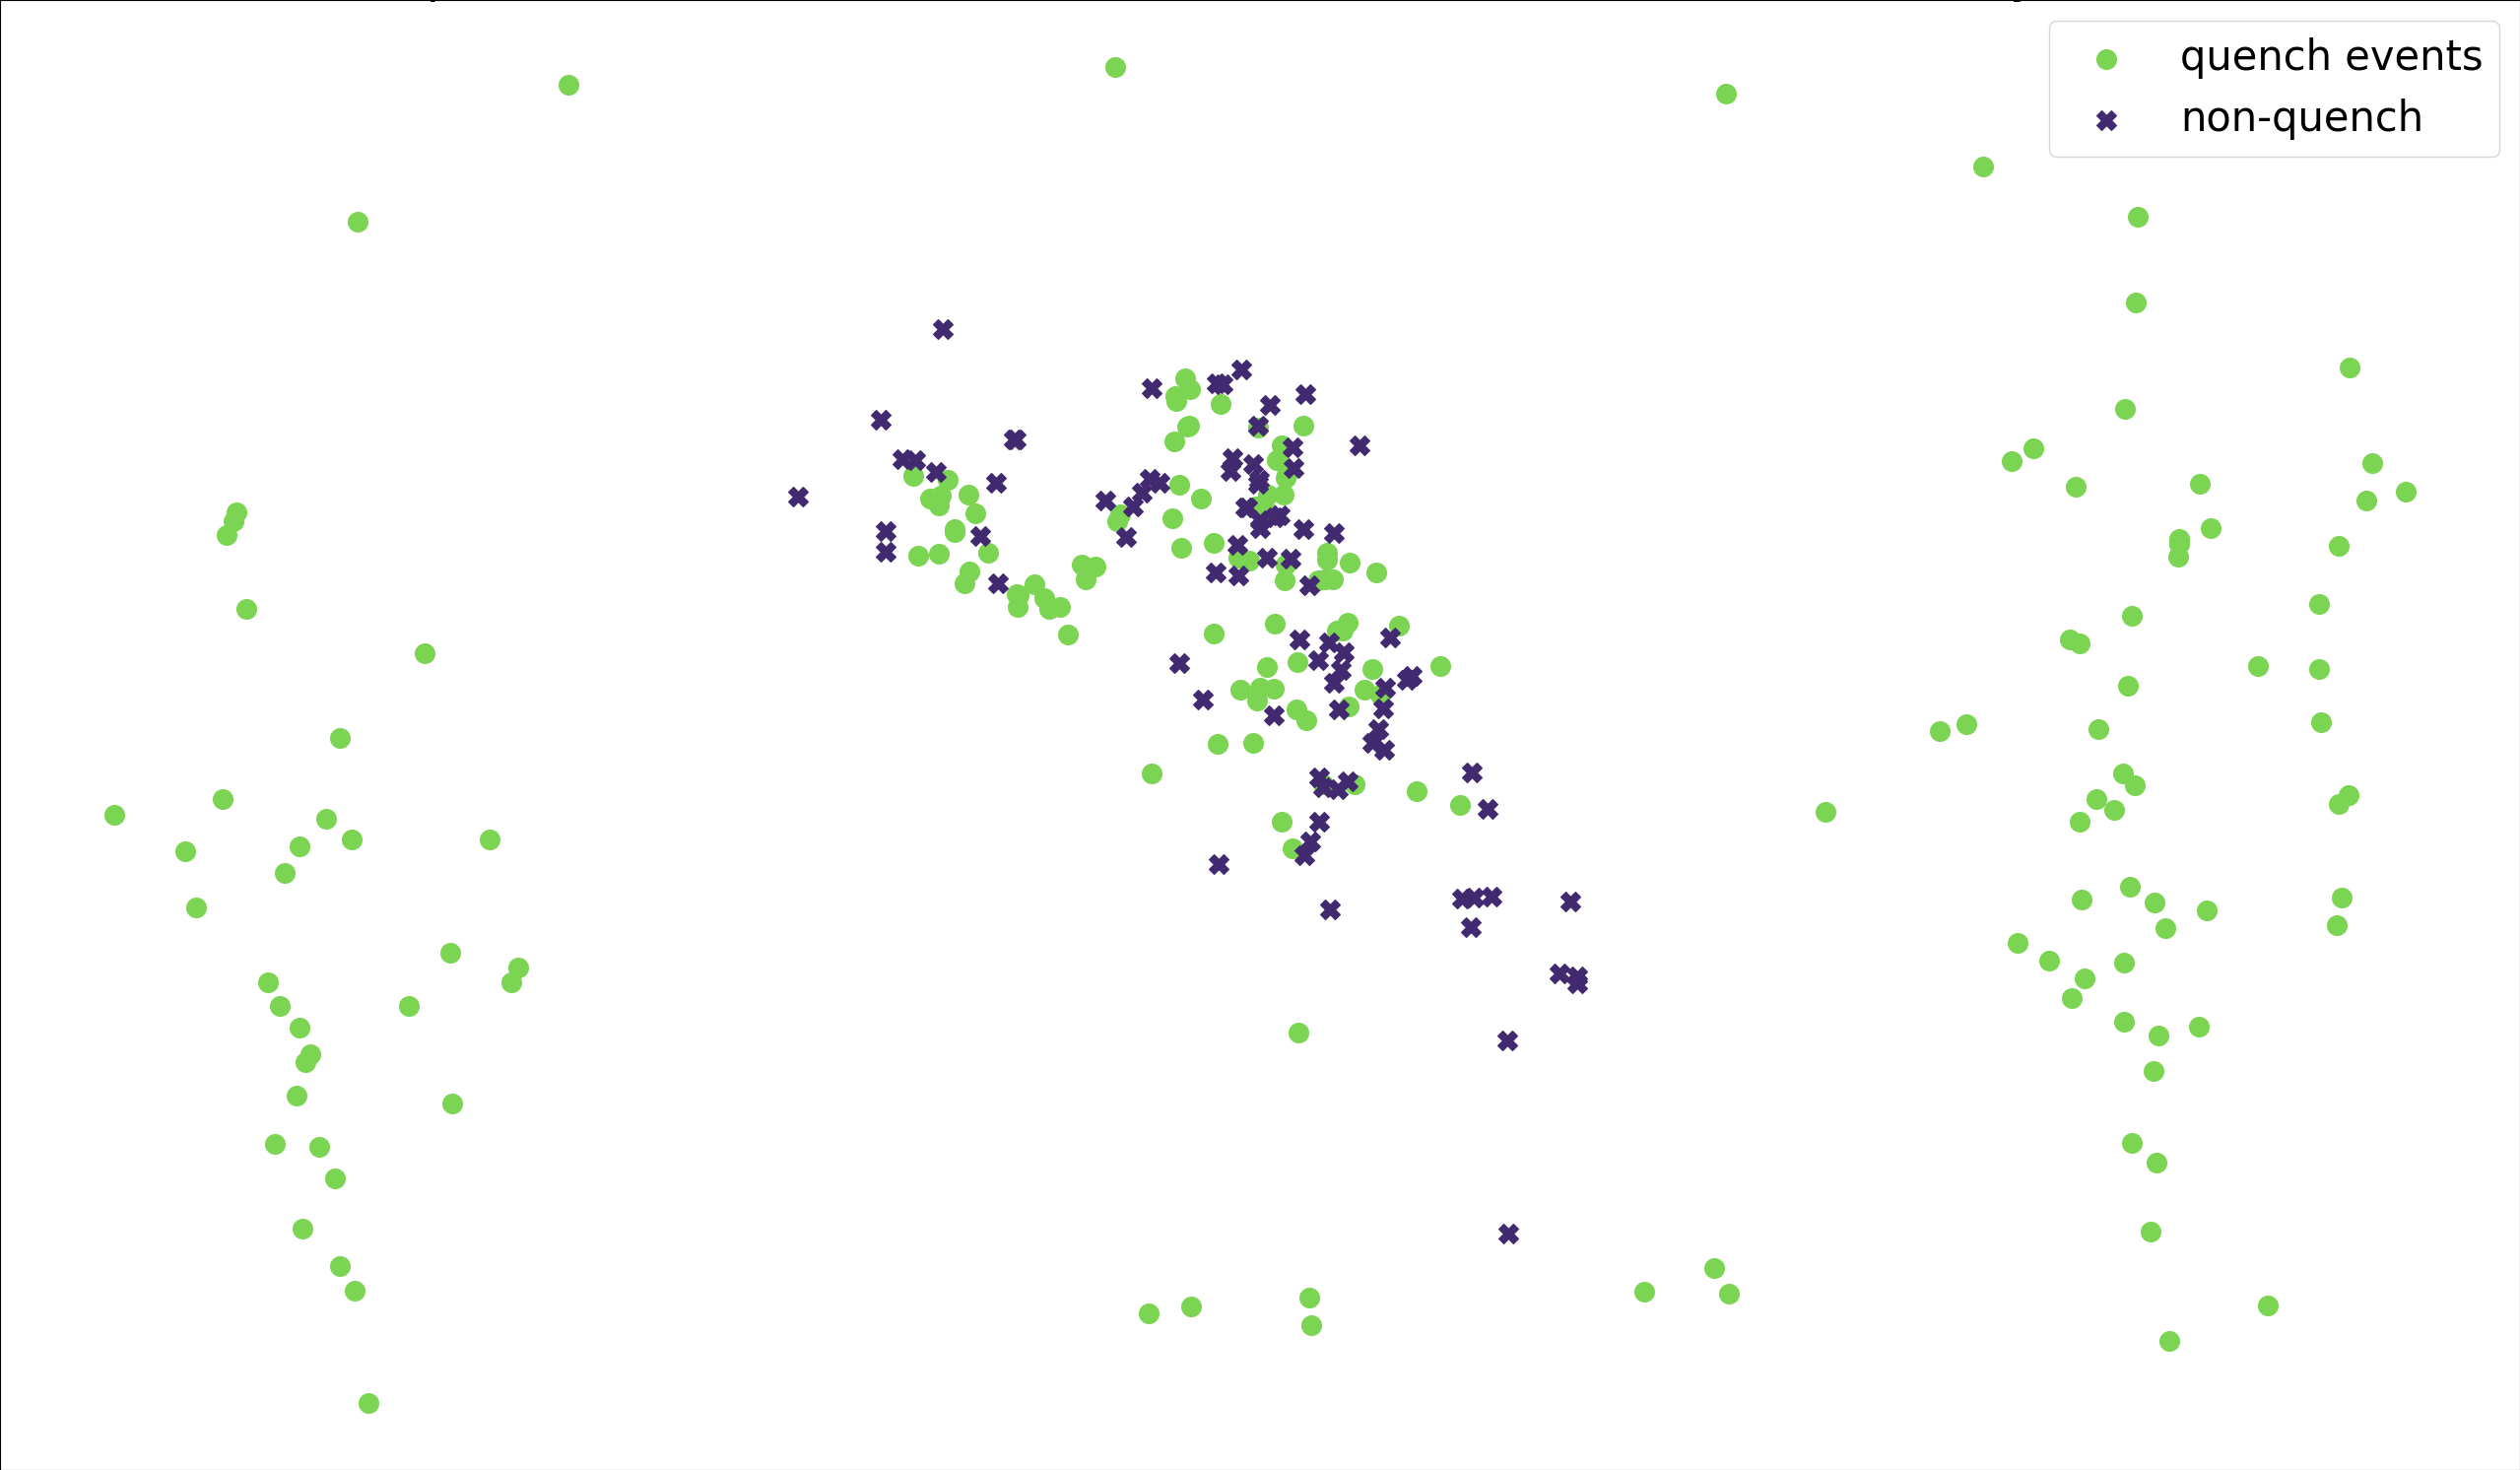
\includegraphics[width=\linewidth]{img/Bn_distribution.png}
	\caption{Data distribution for the \bn\ table after applying \pca\ dimensionality
		reduction, moving from $15$-dimensional space to $2$-dimensional space-dimensional
		space. In the plot we highlight quench and non-quench events.} \label{fig:bn-dist}
\end{figure}

As we did for \an\ we checked the correlation among harmonics for the \bn\ attribute, the results
were very similar, the more striking difference between \Cref{fig:an-corr} and \Cref{fig:bn-corr},
apart from the actual correlation values, is that \bn[2] is not strongly correlated with any other
harmonic (contrarily to \an[2]), while \bn[15] grows a discrete correlation with all odd harmonics.
\begin{figure}[!ht]
	\centering
	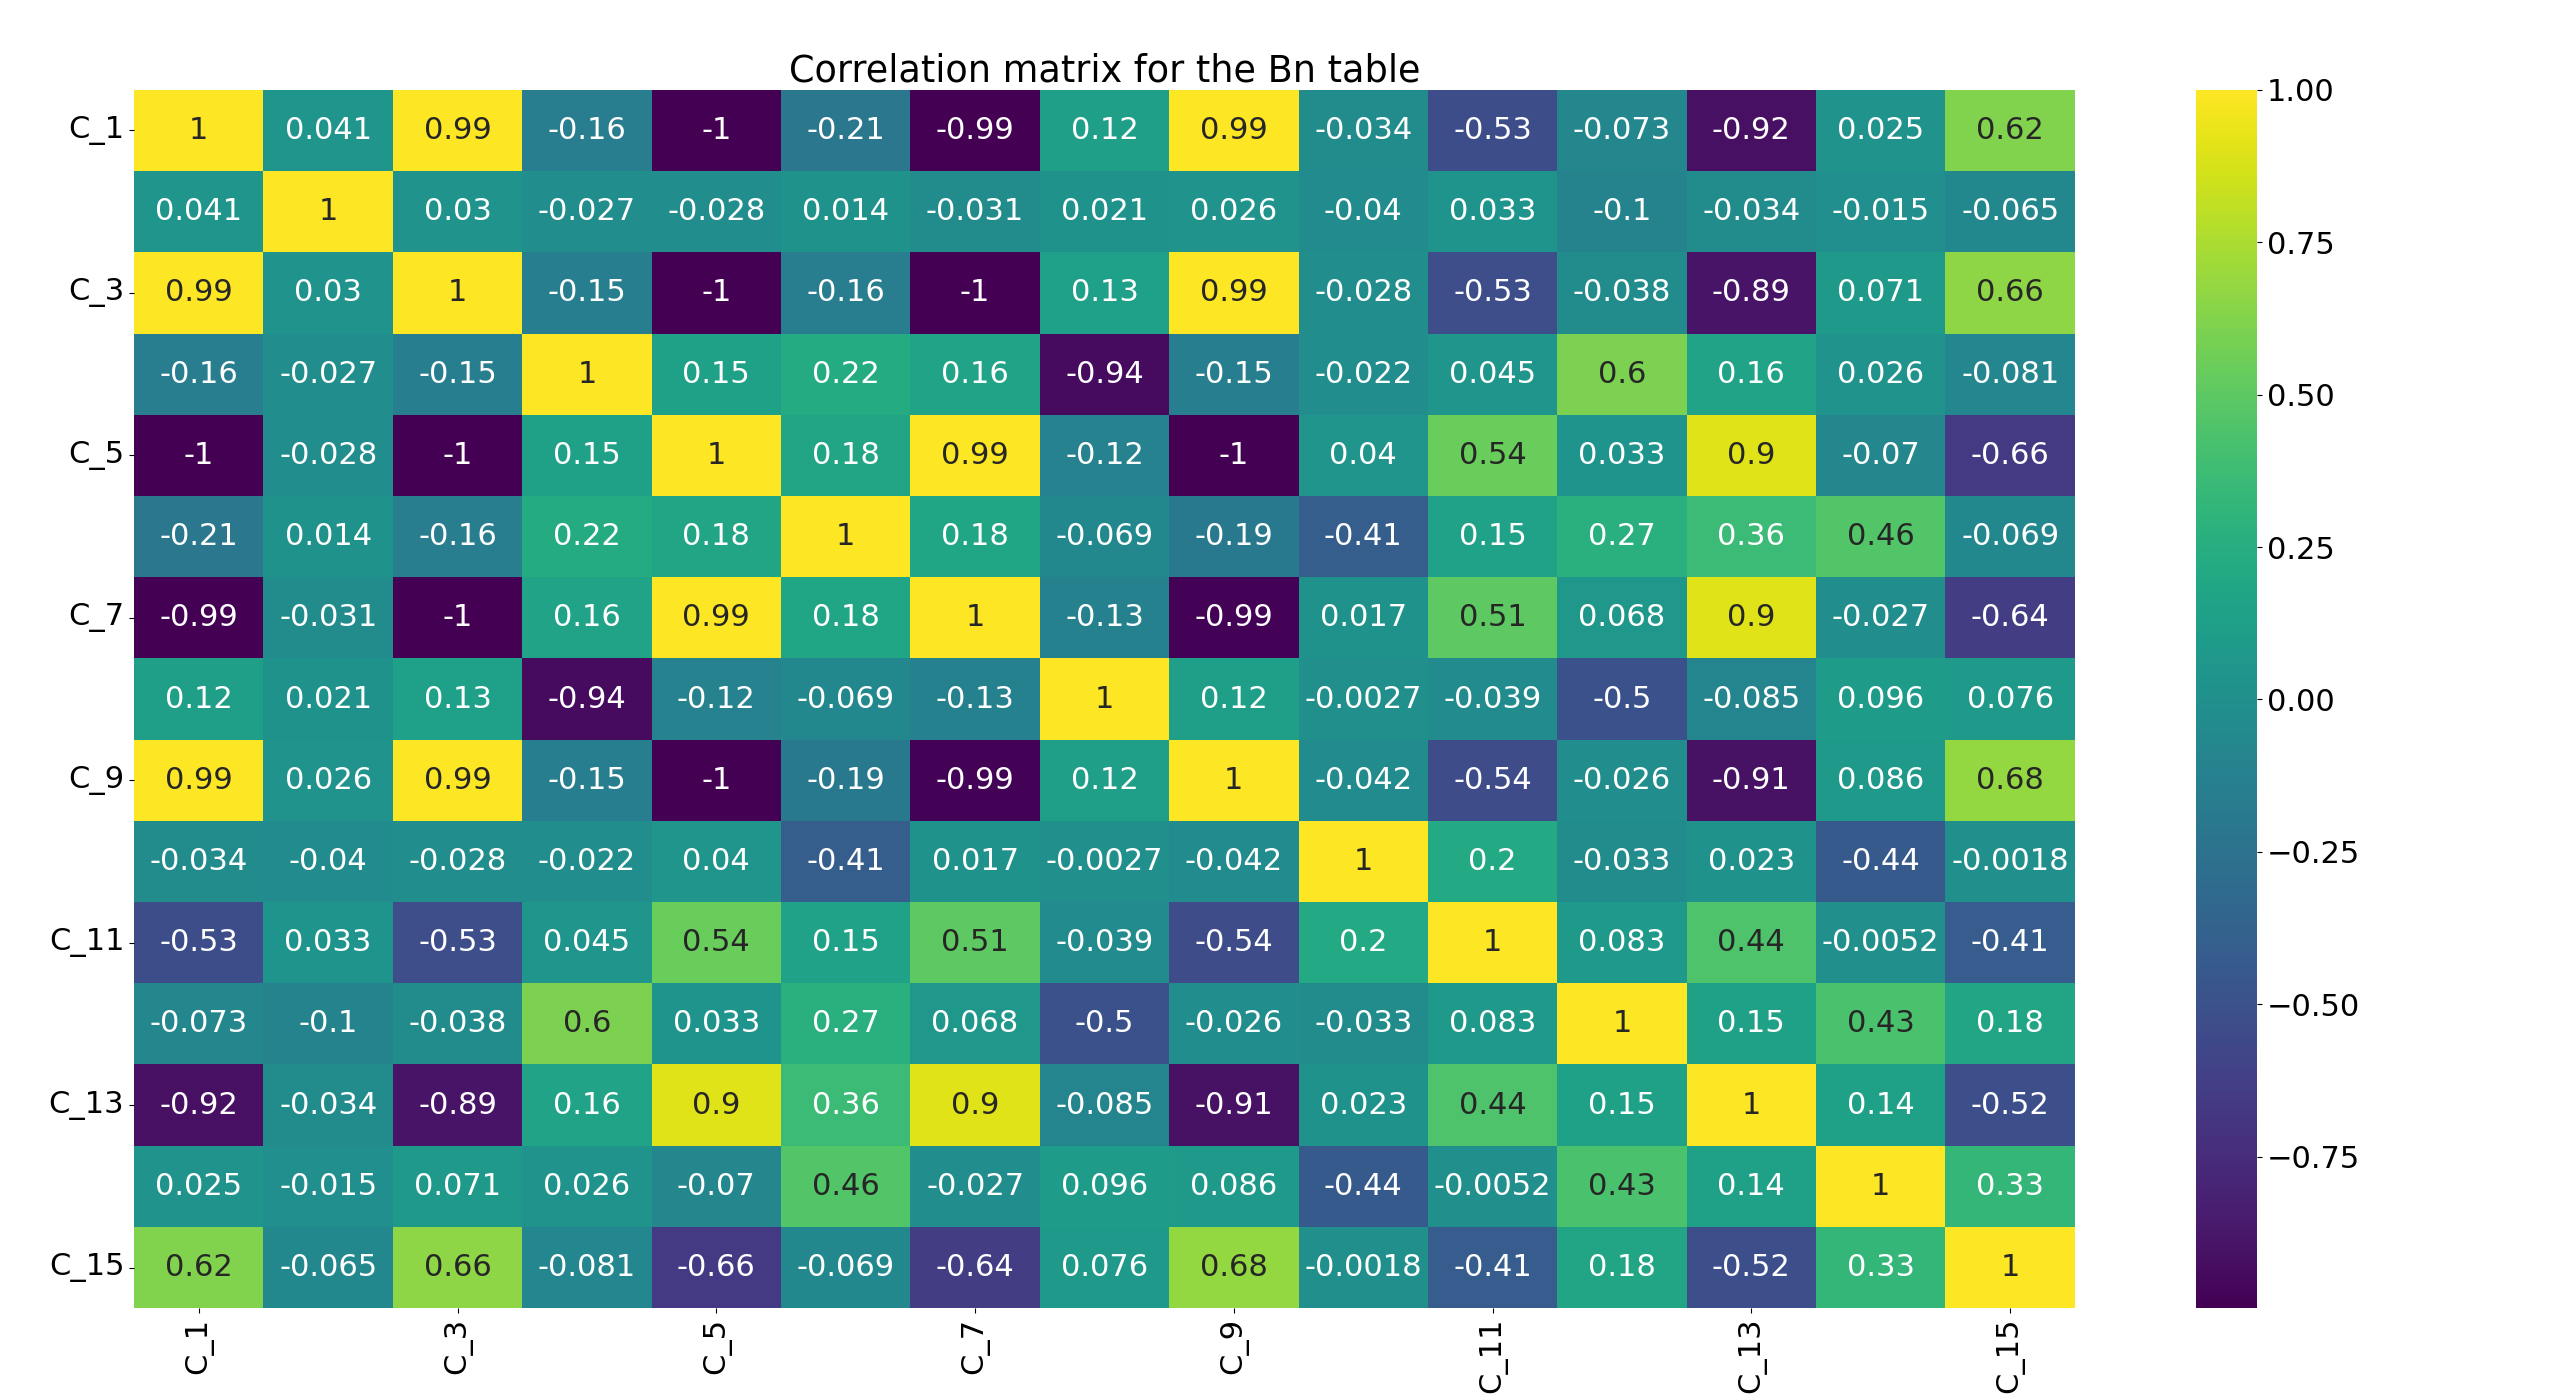
\includegraphics[width=\linewidth]{img/Bn_corr_matrix.png}
	\caption{The cross-correlation among the \bn\ harmonics.} \label{fig:bn-corr}
\end{figure}

If we check the correlation between the harmonics and the labels in (\Cref{fig:bn-lcorr}), we can see
that, apparently, most harmonics have a good enough correlation with the solution, but despite this, the performance of all
models built on \bn\ suffered.
\begin{figure}[!ht]
	\centering
	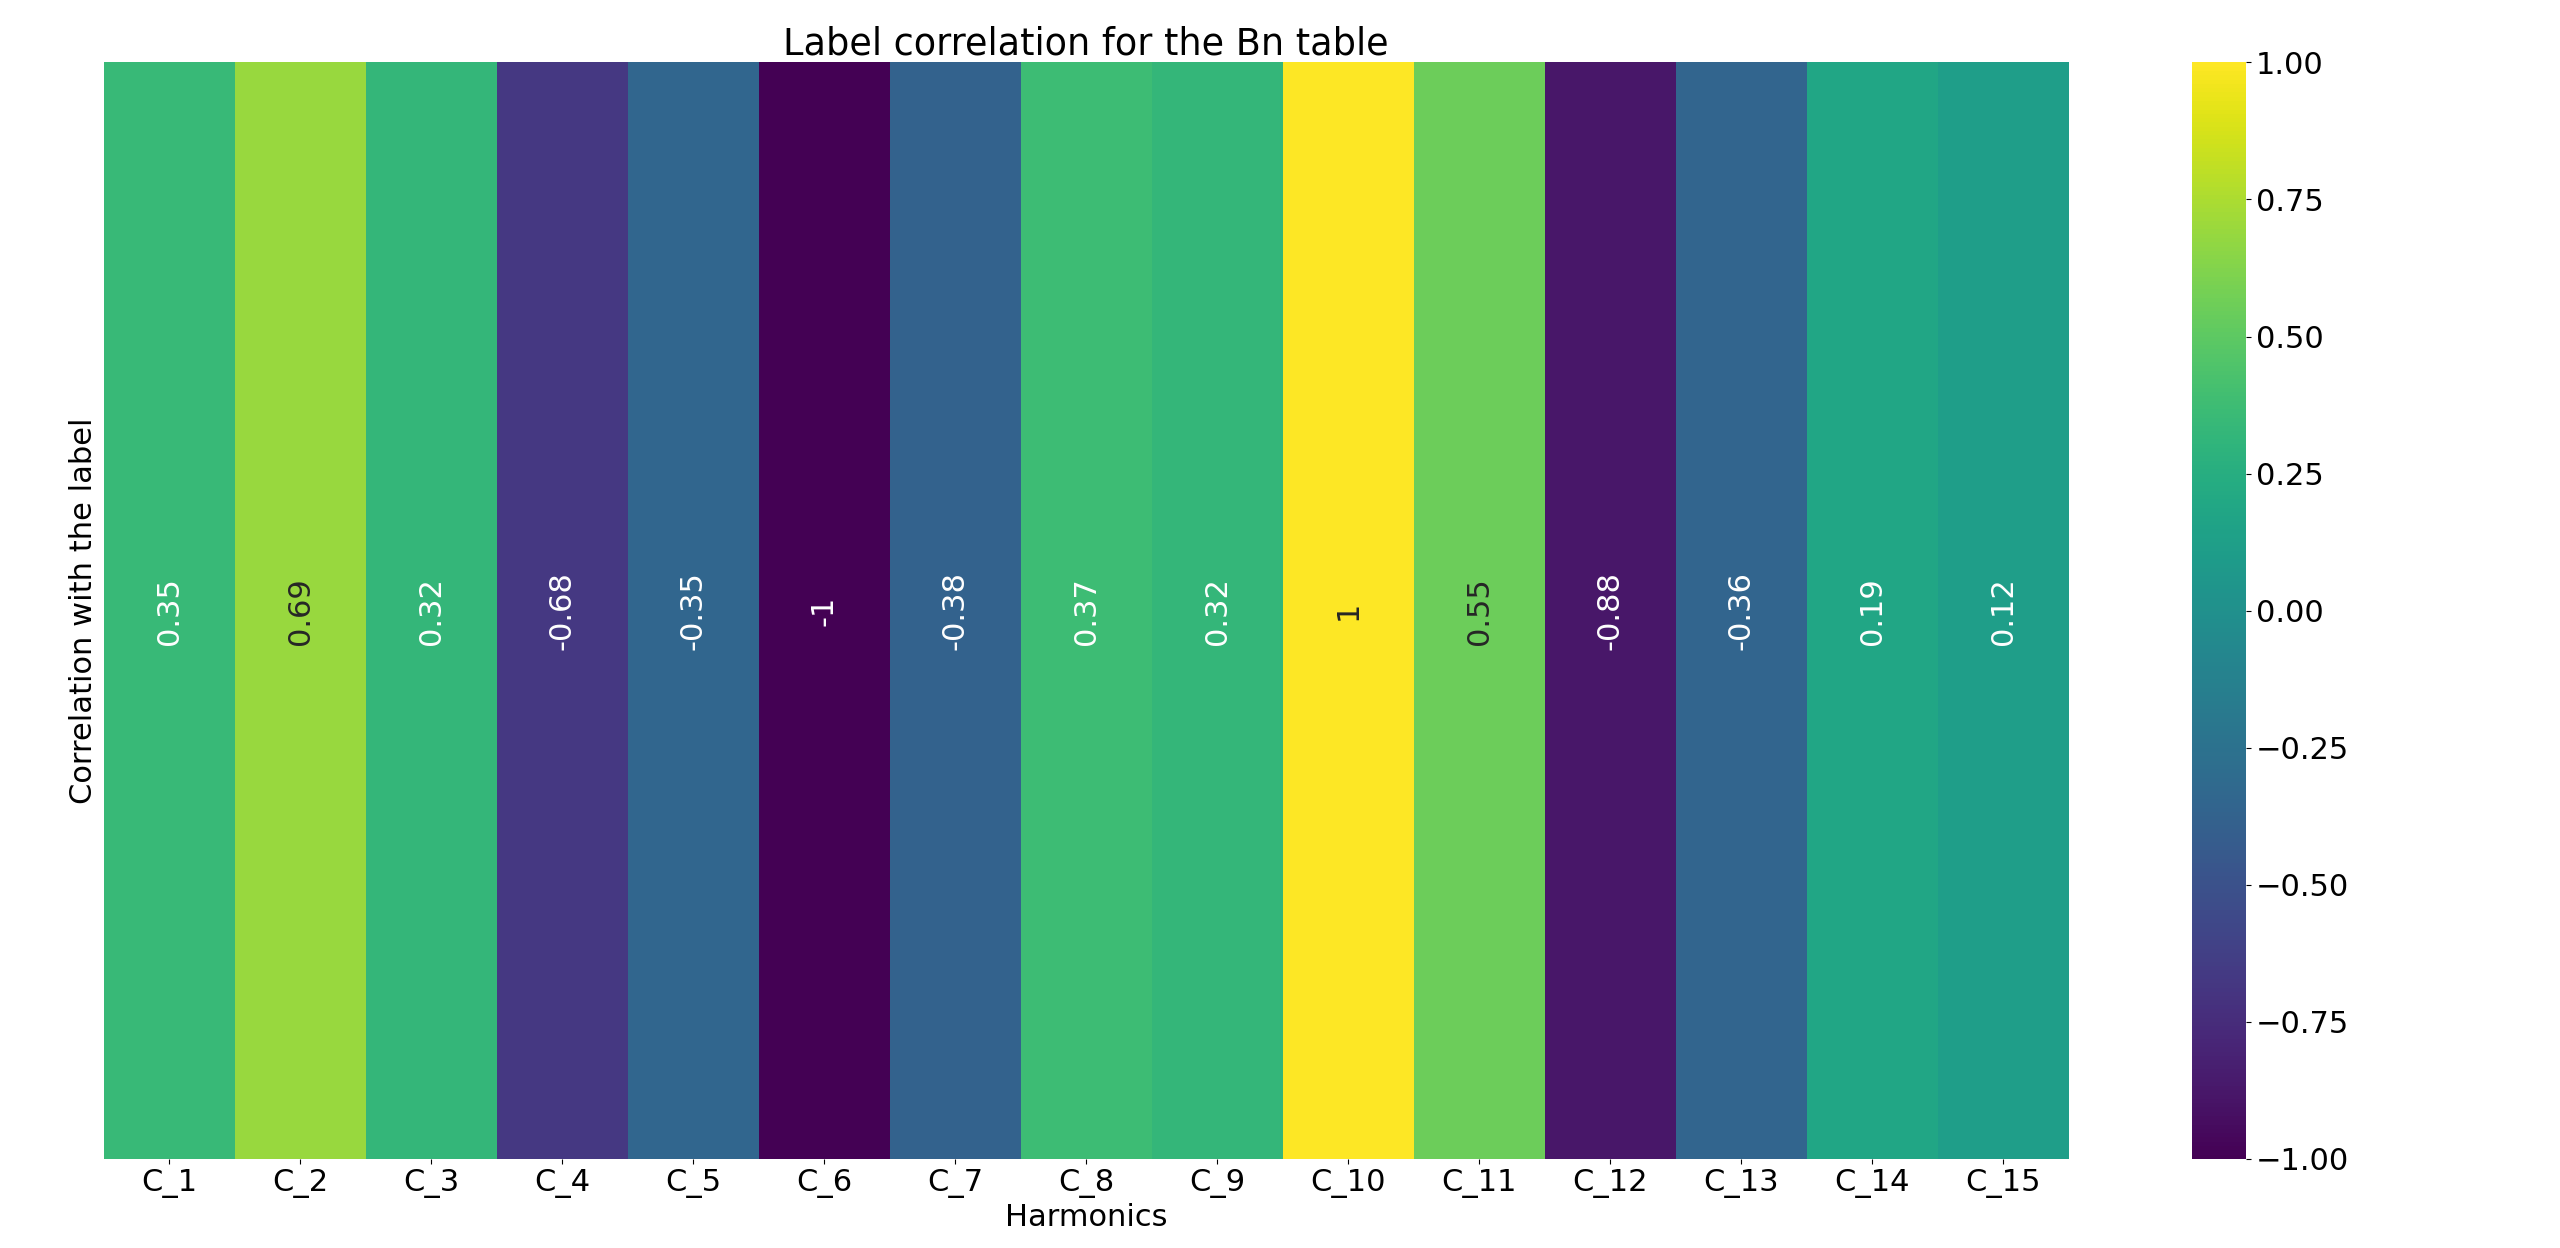
\includegraphics[width=\linewidth]{img/Bn_label_corr.png}
	\caption{Correlation between the harmonics and the labels for \bn.} \label{fig:bn-lcorr}
\end{figure}

\subsubsection{\cnmod}
The \cnmod\ attribute combines the information present in \an\ and \bn, \cnmod\ was expected to be one
of the best tables to solve \qrp, as we highlighted in \Cref{chp:problem}, and, as we will see in
future sections, while models trained on \cnmod\ cannot reach the same level of performance reached
by \an, they are consistently the second-best model available.
\begin{figure}[!ht]
	\centering
	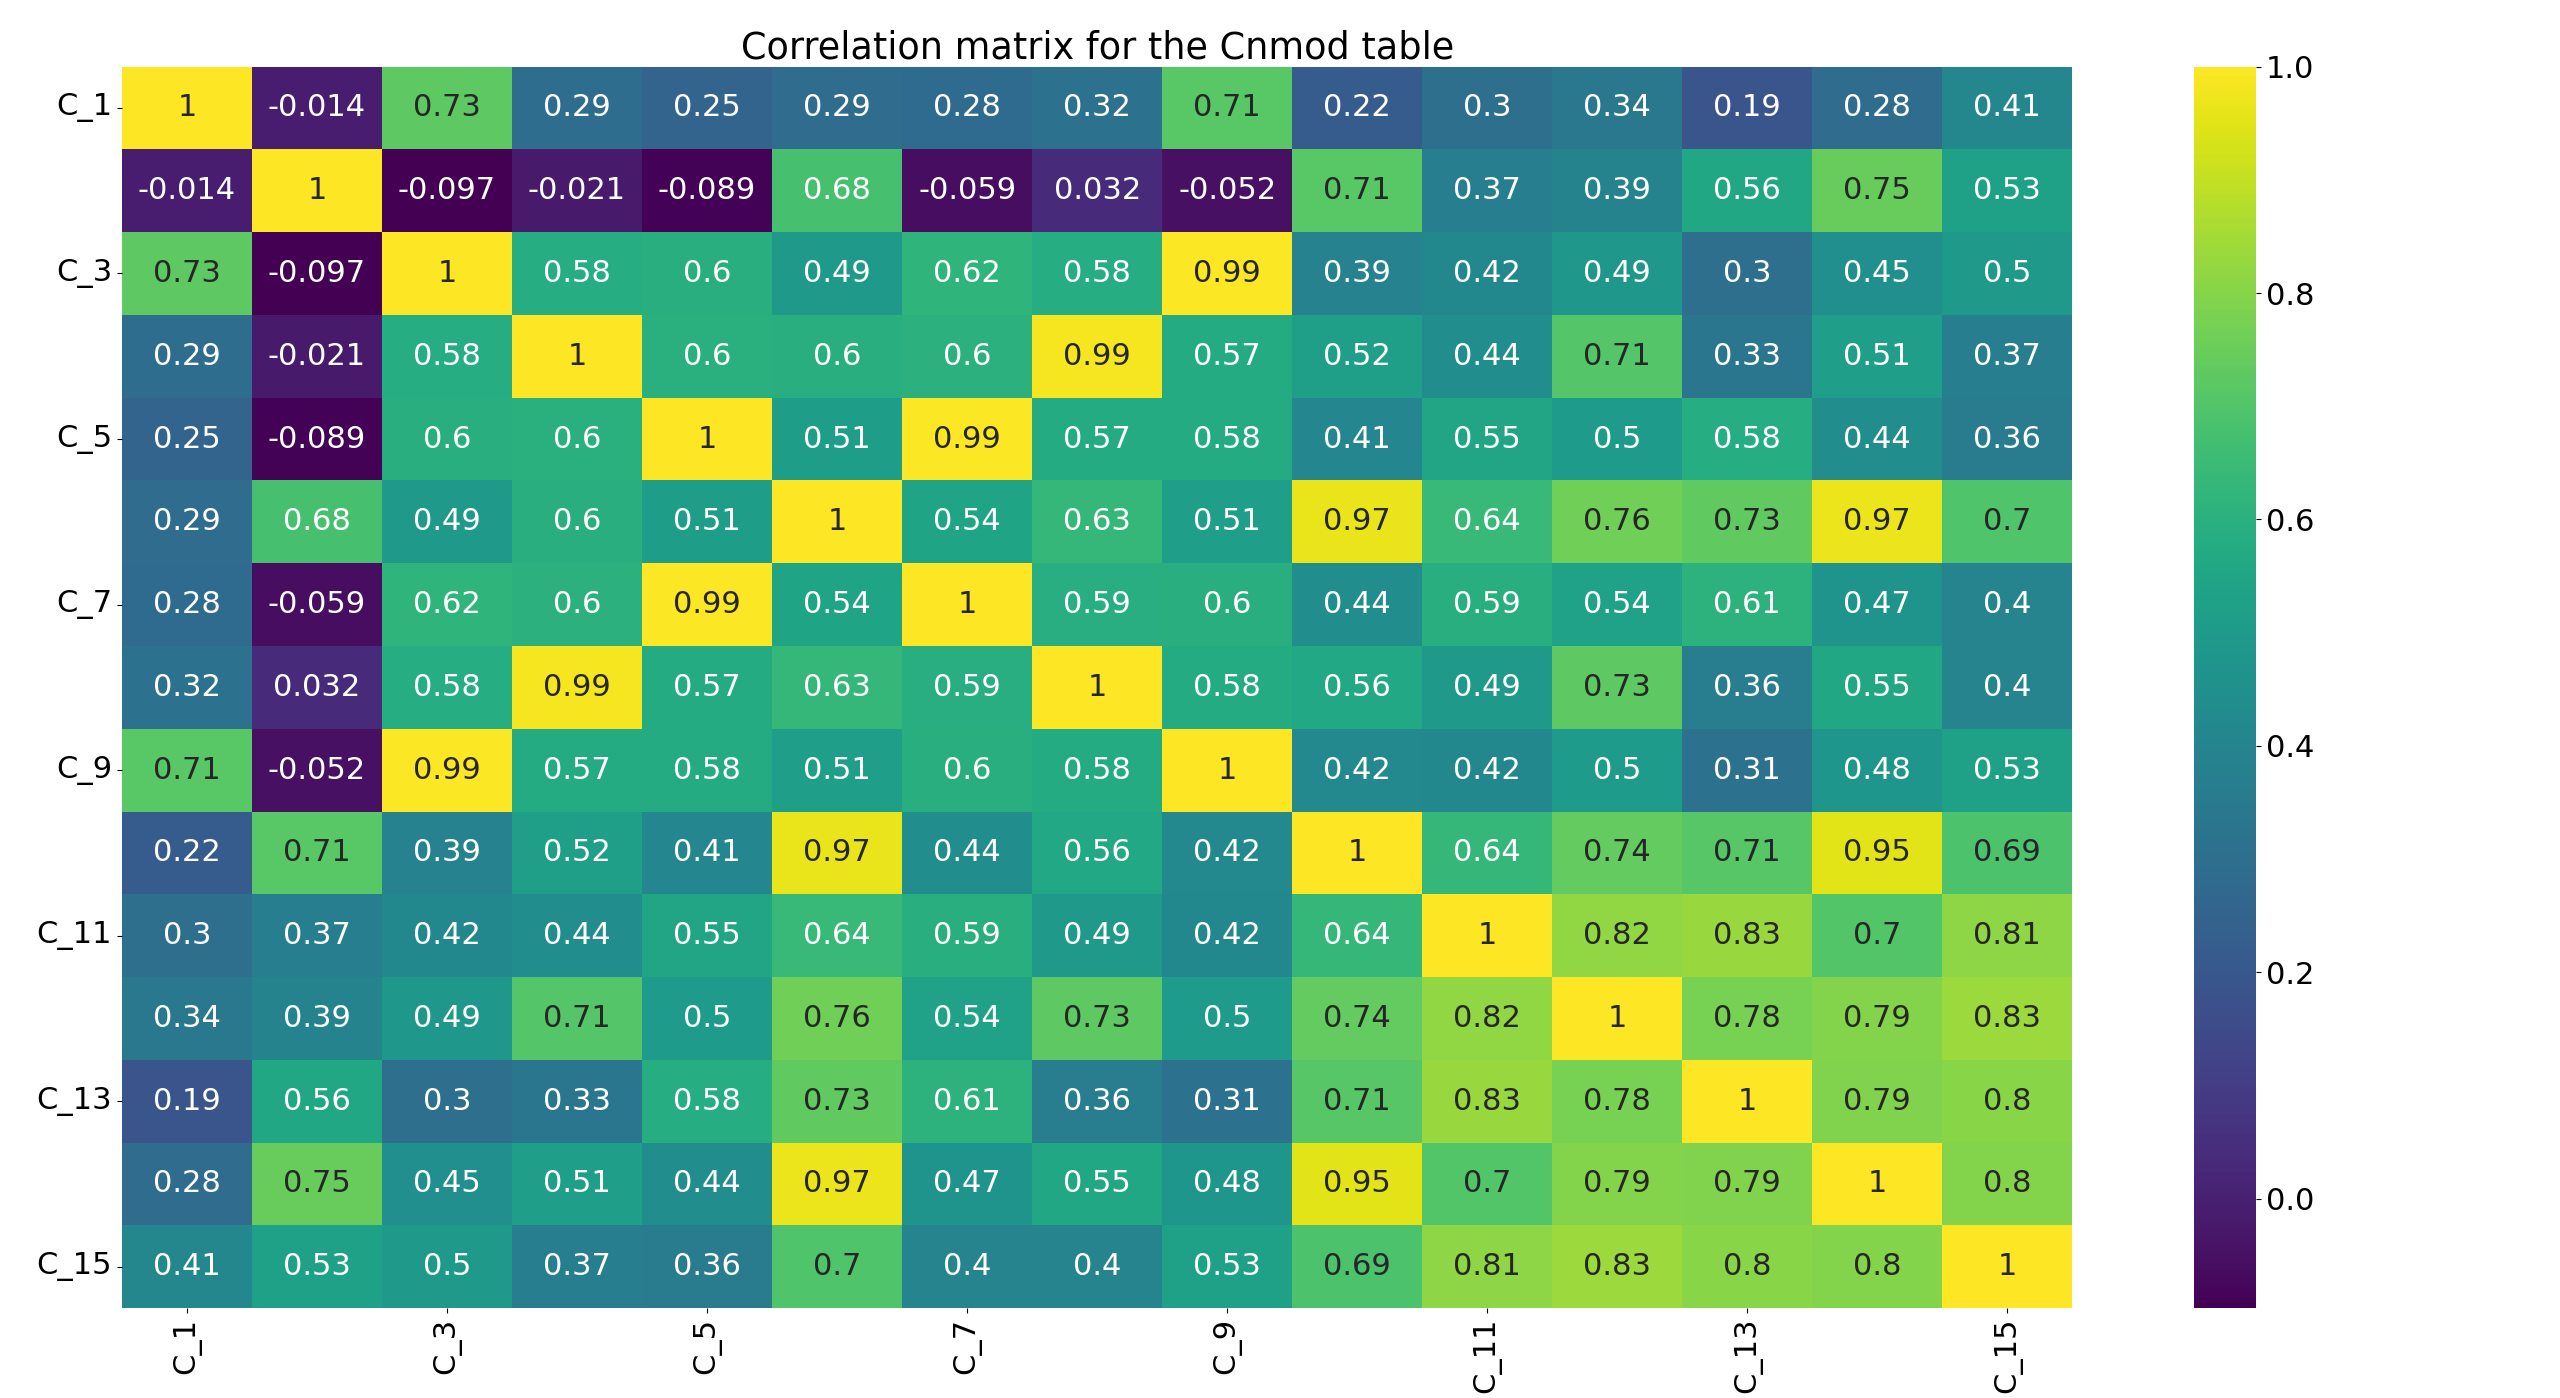
\includegraphics[width=\linewidth]{img/Cnmod_corr_matrix.png}
	\caption{The cross-correlation among the \cnmod\ harmonics.} \label{fig:cnmod-corr}
\end{figure}

\Cref{fig:cnmod-corr} shows the correlation matrix for \cnmod, its structure is very complicated,
since:
\begin{itemize}
	\item \cnmod[2] is strongly correlated with all harmonics until \cnmod[9],
	\item Harmonics between \cnmod[10] and \cnmod[15] are strongly correlated among themselves,
	\item \cnmod[4] is strongly correlated with its multiples.
\end{itemize}
\begin{figure}[!ht]
	\centering
	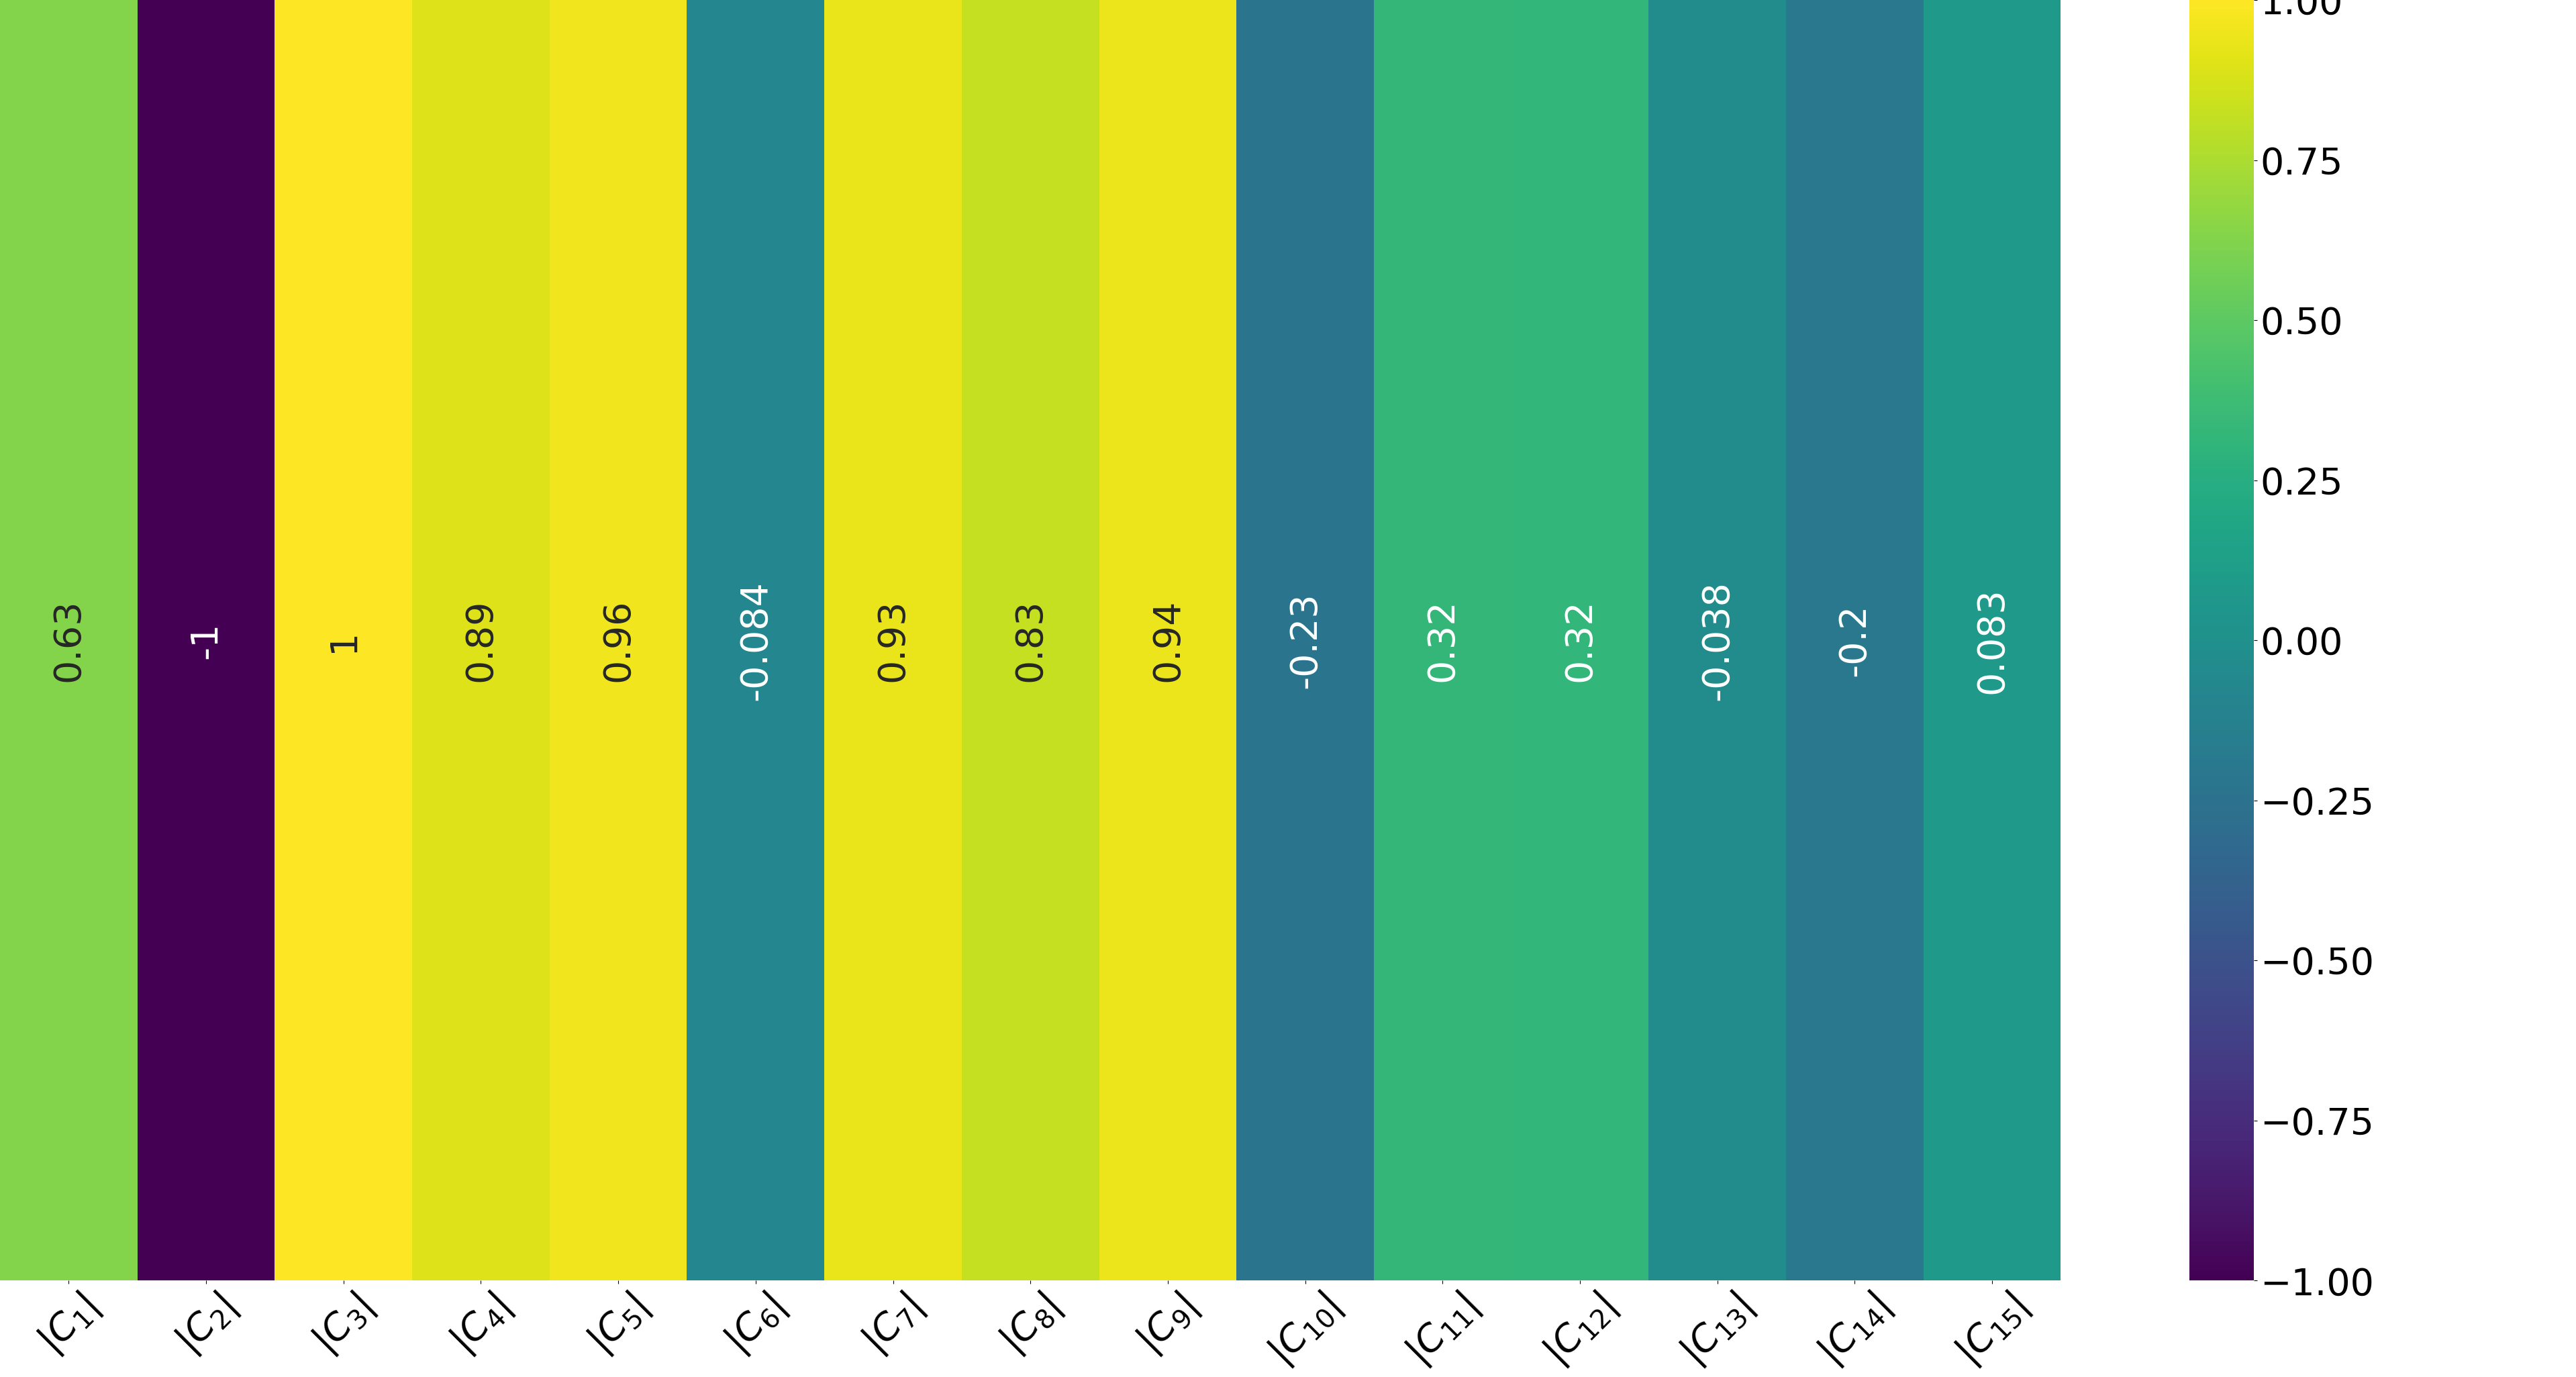
\includegraphics[width=\linewidth]{img/Cnmod_label_corr.png}
	\caption{Correlation between the harmonics and the labels for \cnmod.} \label{fig:cnmod-lcorr}
\end{figure}

Looking at both \Cref{fig:cnmod-corr} and \Cref{fig:cnmod-lcorr}, we can conclude that two different
approaches can be followed:
\begin{itemize}
	\item Using \cnmod[2] alongside one or more high-order harmonics,
	\item Using \cnmod[3] and some other low-order harmonics (potentially even the
	      first one) alongside one high-order harmonic (e.g., \cnmod[14]).
\end{itemize}
Analyzing the boxplot suggested that using harmonic number \cnmod[2] was not promising, due to the extreme
concentration of the data.

\Cref{fig:cnmod-dist} visualizes the distribution of the samples in \cnmod\ after a round of \pca,
the samples are characterized by a good enough distribution, we could easily identify clusters with
a high degree of purity, apart from the one in the leftmost region of the image, which contains
samples belonging to both classes mixed together homoegeneously. In the rightmost part of the image
we can identify a sample which can be considered an outlier and was removed whenever we experimented
clustering approaches. Overall \cnmod\ doesn't have a distribution quite as good as \an\ did, but comparing it to \Cref{fig:bn-dist} or \Cref{fig:phi-dist}, has a much better topology.
\begin{figure}[!ht]
	\centering
	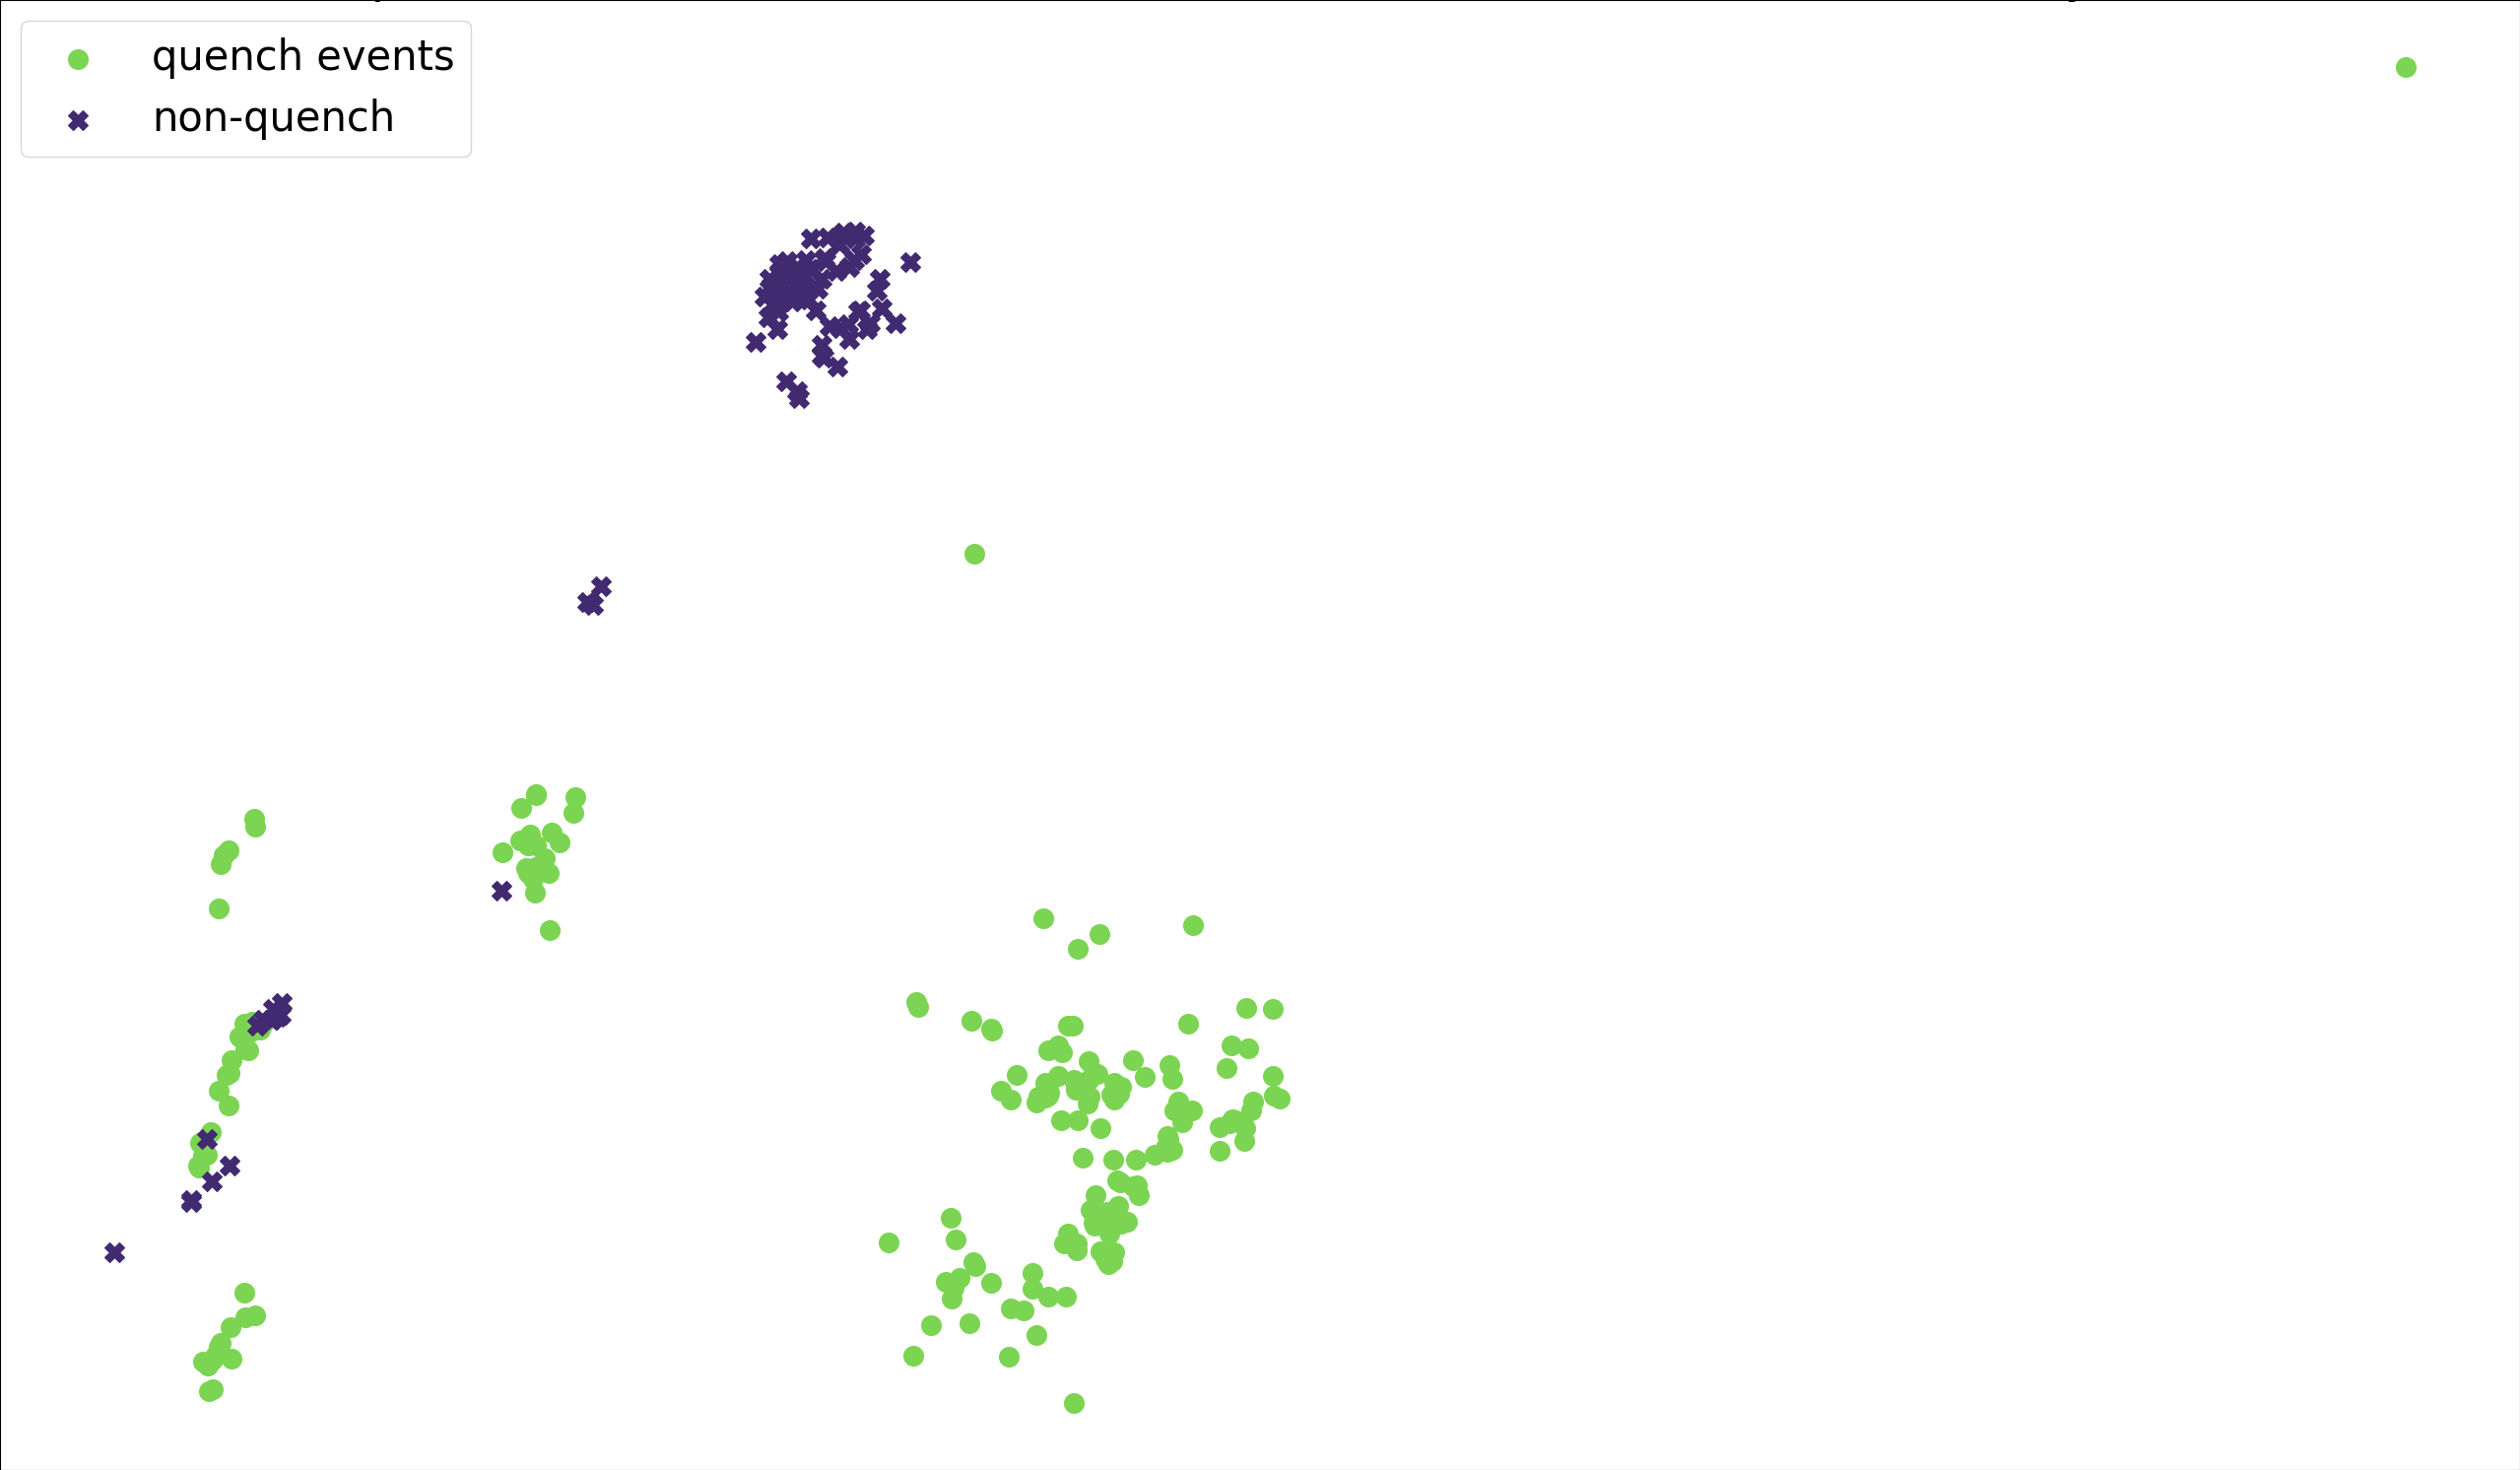
\includegraphics[width=\linewidth]{img/Cnmod_distribution.png}
	\caption{Data distribution for the \cnmod\ table after applying \pca\ dimensionality
		reduction, moving from $15$-dimensional space to $2$-dimensional space-dimensional
		space. In the plot we highlight quench and non-quench events.} \label{fig:cnmod-dist}
\end{figure}

\subsubsection{\phin}
As we will see in further sections the \phin-based models consistently outperformed the ones based
on \bn. As we saw with \bn, also in the case of \phin, the data distribution after a round of \pca,
shown in \Cref{fig:phi-dist}, is characterized by a series of high-impurity clusters, where samples of the two classes are mixed together.

\begin{figure}[!ht]
	\centering
	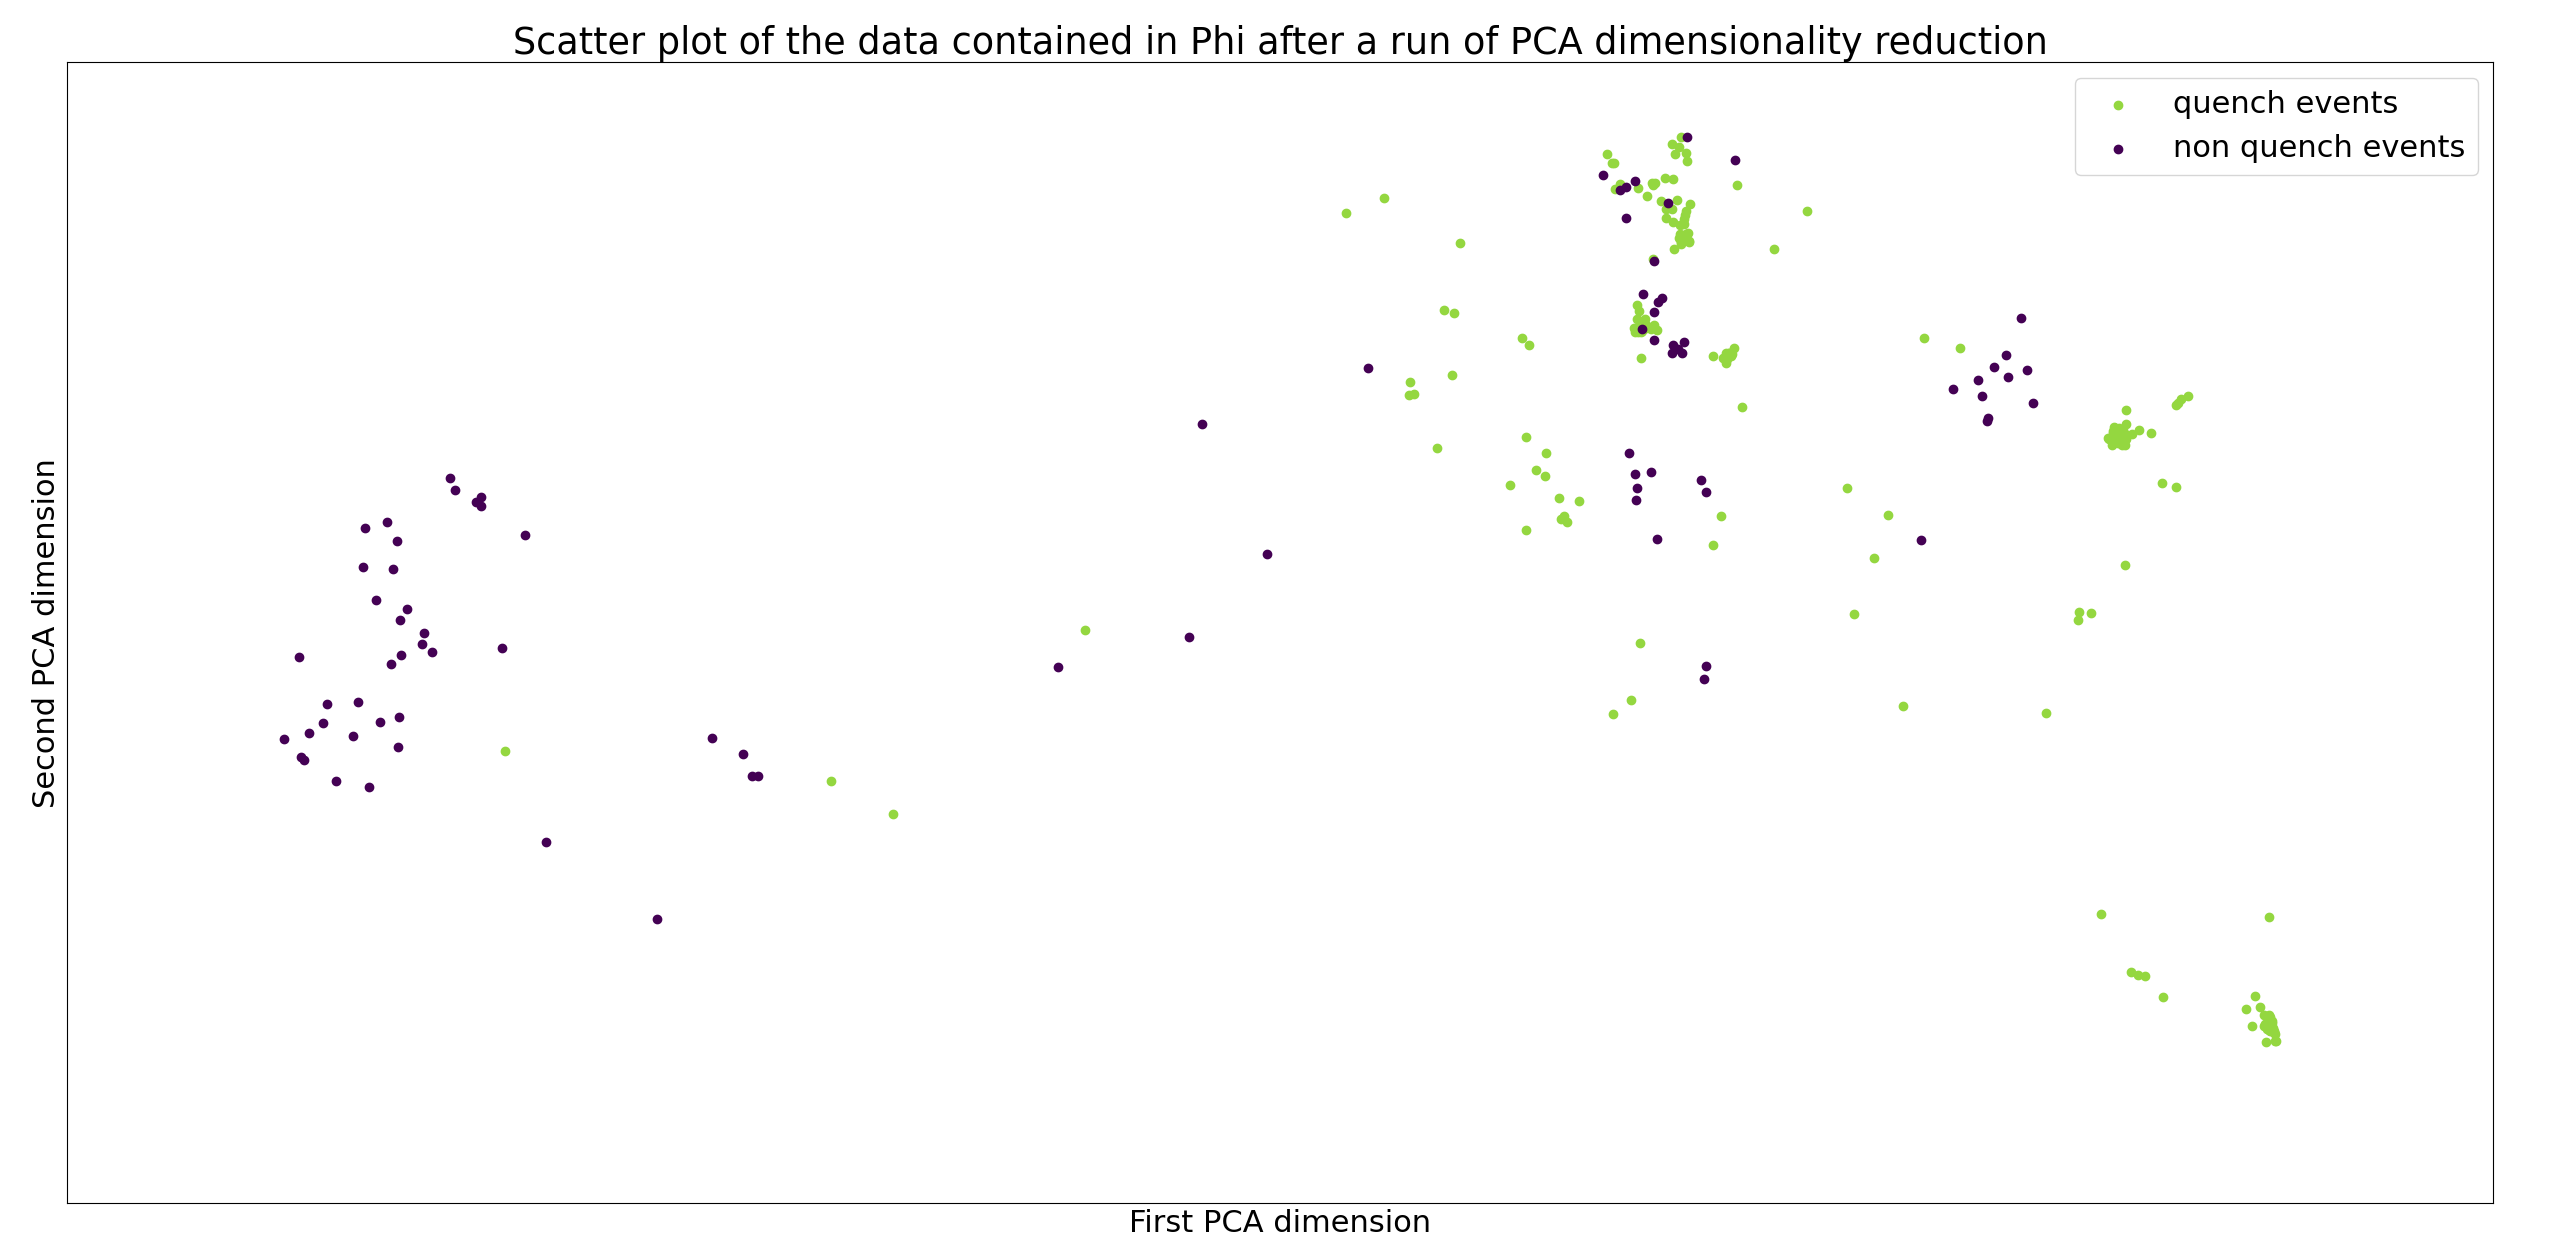
\includegraphics[width=\linewidth]{img/Phi_distribution.png}
	\caption{Data distribution for the \phin\ table after applying \pca\ dimensionality
		reduction, moving from $15$-dimensional space to $2$-dimensional space-dimensional
		space. In the plot we highlight quench and non-quench events.} \label{fig:phi-dist}
\end{figure}

In \Cref{fig:phi-corr} we plotted the correlation matrix for \phin, contrarily to the correlation
matrix of other attributes, the amount of harmonics that are strongly correlated with each other is very
low (only \phin[2] and its odd multiples and \phin[4] and its multiples). Compared to the
aforementioned attributes the matrix contains no real structure.
\begin{figure}[!ht]
	\centering
	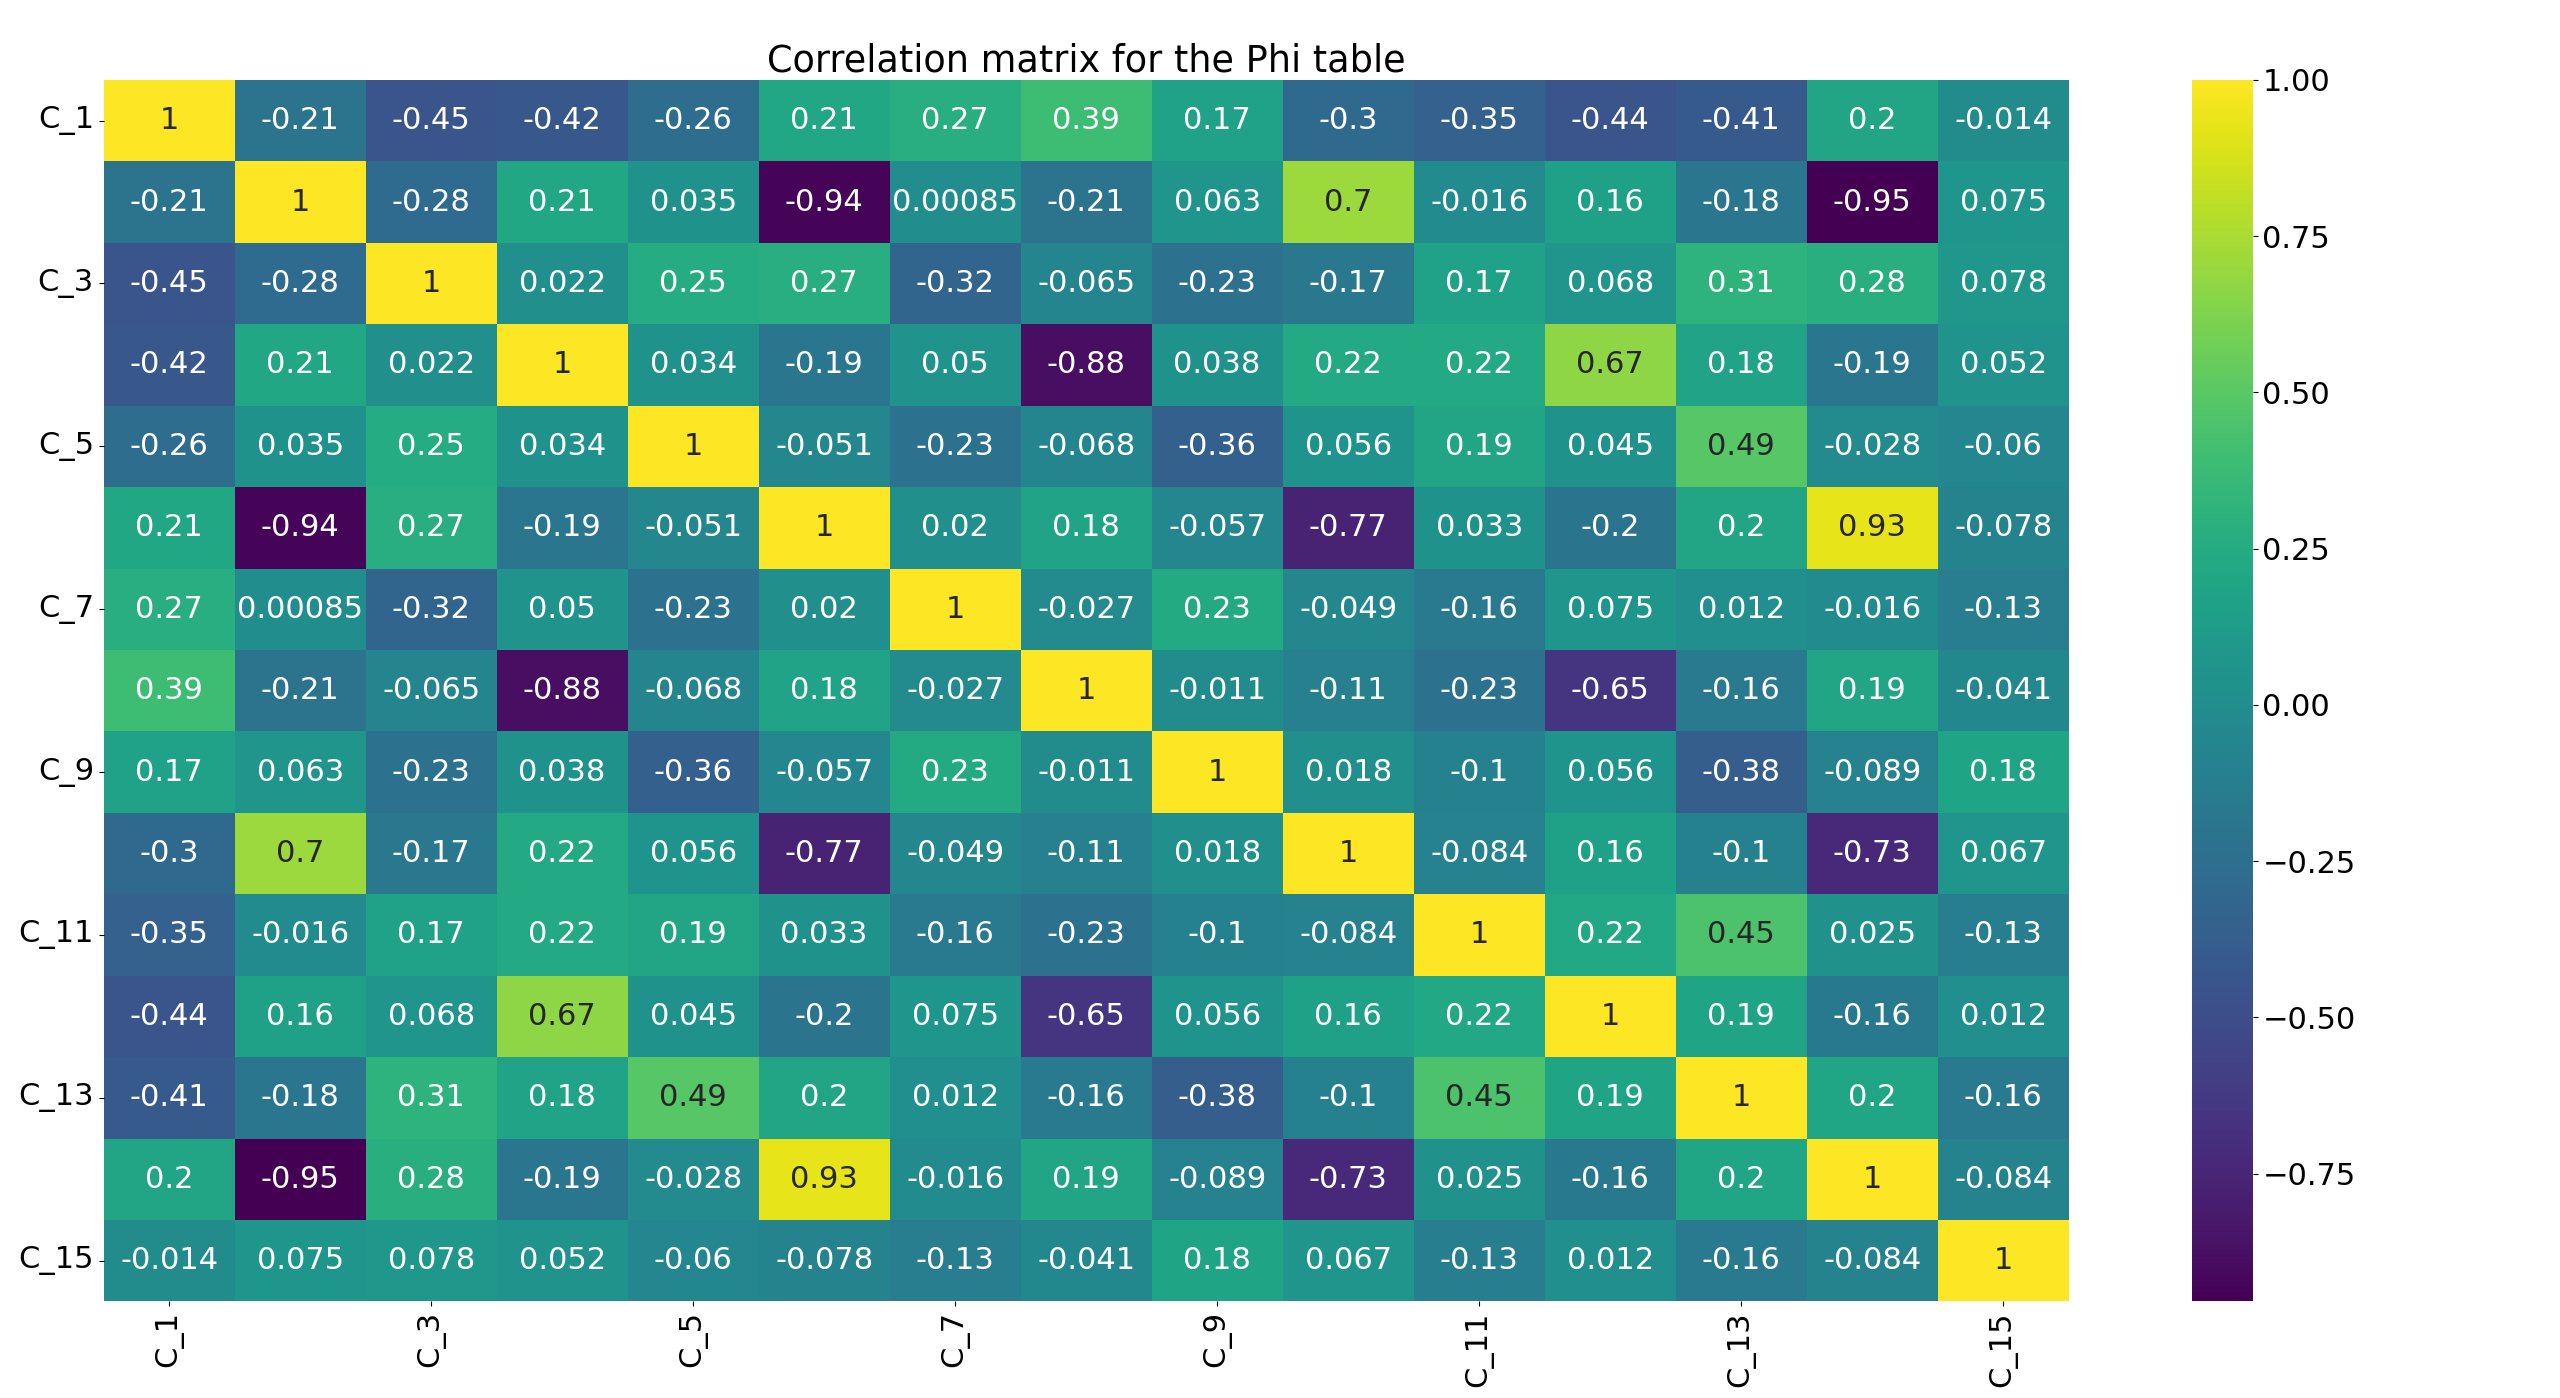
\includegraphics[width=\linewidth]{img/Phi_corr_matrix.png}
	\caption{The cross-correlation of the \phin\ harmonics} \label{fig:phi-corr}
\end{figure}
Whenever we choose to use \phin\ to build datasets we are left with much more freedom during the
feature extraction process, the only things that really stand to the eye are that:
\begin{inparaenum}[(i)]
	\item Harmonic number $2$ is strongly correlated with its odd multiples,
	\item harmonic number $4$ is strongly correlated with its multiples.
\end{inparaenum}

Lastly, we can analyze the correlation between the harmonics and the label. As we can see in \Cref{fig:phi-lcorr} most of the harmonics have a good correlation with the expected solution, especially harmonic number $2$ and its odd multiples, and harmonics number $1$ and $12$.
\begin{figure}[!ht]
	\centering
	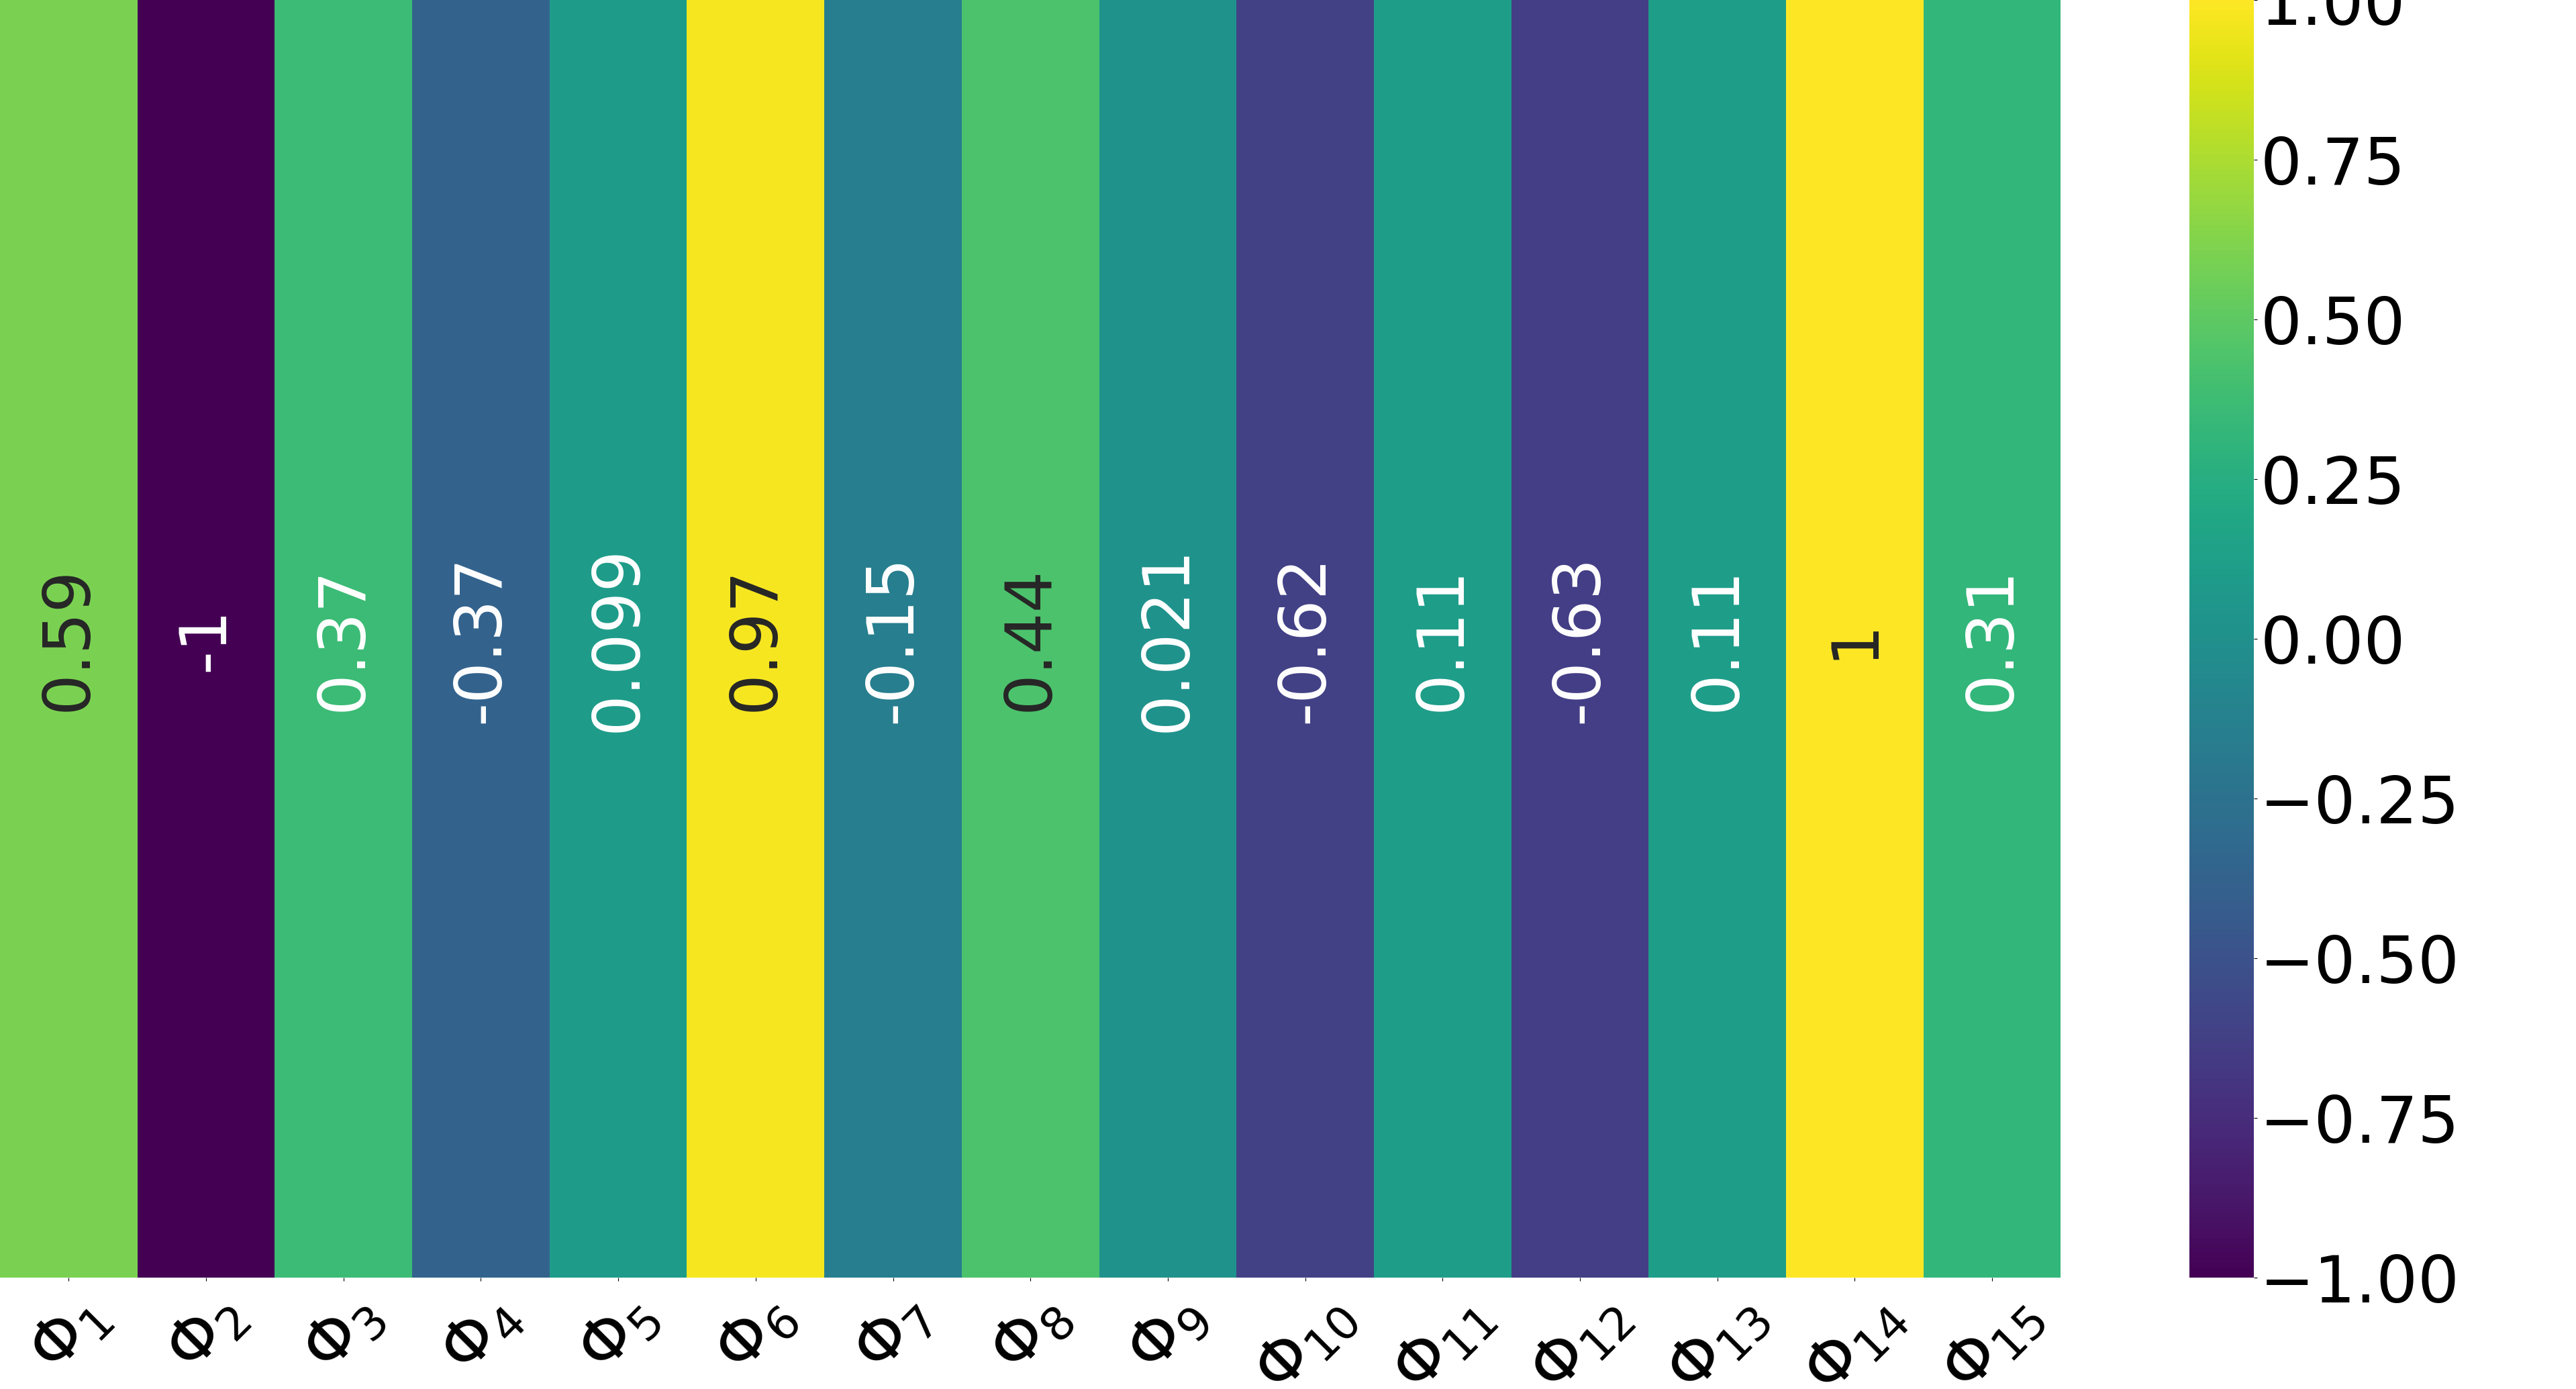
\includegraphics[width=\linewidth]{img/Phi_label_corr.png}
	\caption{Label correlation for the \phin\ table} \label{fig:phi-lcorr}
\end{figure}

This closes the brief exposition about the preprocessing steps for the various labels, now we will
tackle the model selection procedure indicating which were the best models overall and which model
we chose to solve \qrp.

\section{Results}
\label{sec:results-qrp}
Every model shown in this section has been tested using the pipeline that we introduced in
\Cref{chp:problem}. In this chapter we will proceed as we did in \Cref{chp:ml} for the theoretical
introduction of the models, therefore:
\begin{itemize}
	\item The first subsection delineates the performance of decision trees,
	\item The second subsection delineates the performance of random forests,
	\item The third subsection delineates the performance of our benchmarking model, the \svm,
	\item The last subsection will introduce the tree aggregator model
\end{itemize}
At the end of the chapter we will talk about the best performing model and we will give the final
results for \qrp.

\subsection{Decision trees}
\label{sec:qrp-dt}
As we already alluded to in previous sections we wanted to find a highly explainable model with good
performance that could be used to solve \qrp, that is exactly why the development process started
with \dts.

With our experiments we tried different approaches and different datasets, after a careful analysis
and many experiments we found that the best \dts were all based on \an, the confusion matrix for
the best model, trained on harmonics $2$ and $12$, is shown in \Cref{fig:dt-an-2-12-cm}, as we can
see, the total number of errors made by the model is of only $4$ total, $3$ false negatives and $1$
false positive.
\begin{figure}[h!]
	\centering
	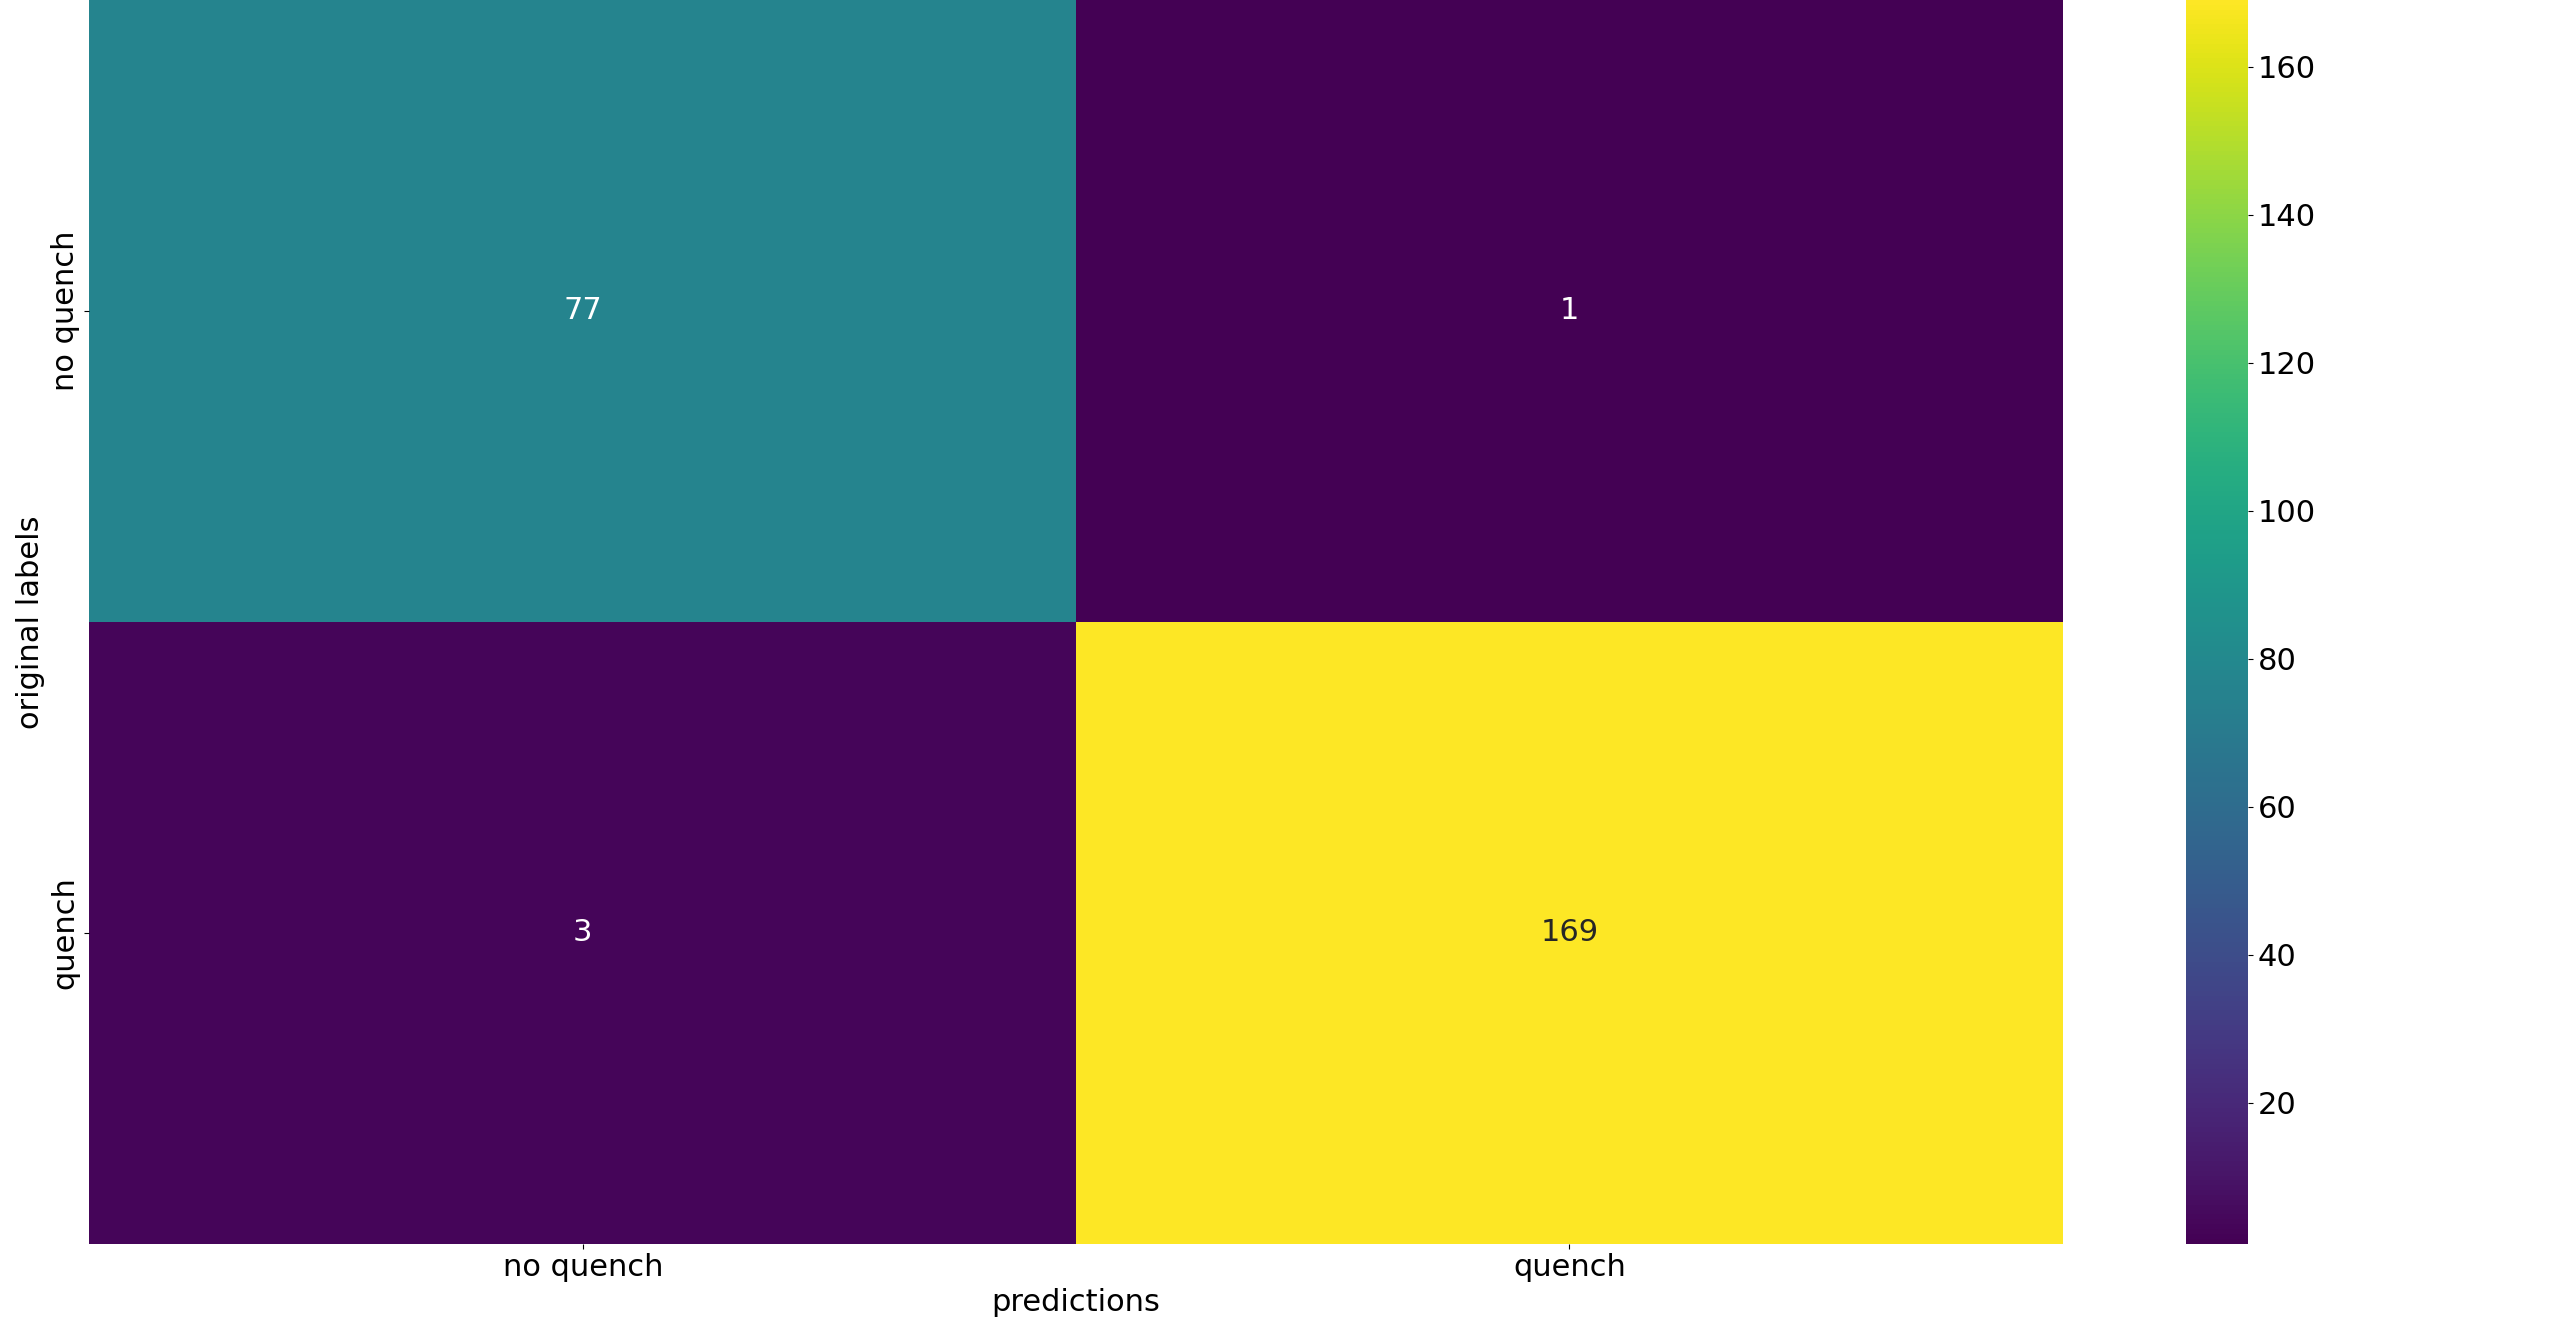
\includegraphics[width=\linewidth]{img/An_2_12_cm_dt.png}
	\caption{The performance for the \an model built on harmonics $2, 12, 15$}
	\label{fig:dt-an-2-12-cm}
\end{figure}
The average performance of the model over the outer \cv\ folds is reported in \Cref{tbl:an-2-12-perf},
as we can see, the numbers are already very solid, showing high average fold performance and low
standard deviation.
\begin{table}[t]
	\caption{Average and standard deviation of the performance for the best \dt\ over the outer \cv\
		fold.}\label{tbl:an-2-12-perf}

	\bigskip
	\setlength{\tabcolsep}{6pt}
	\centering
	\begin{tabular}{ccccccc}
		\toprule
		\textbf{}    & \textbf{Acc} & \textbf{Prc} & \textbf{Rec} & \textbf{Irec} & \textbf{F1} & \textbf{RAUC} \\
		\midrule
		Mean         & 0.984        & 0.994        & 0.983        & 0.988         & 0.988
		             & 0.989                                                                                    \\
		\textsc{std} & 0.008        & 0.011        & 0.014        & 0.025         & 0.006
		             & 0.012                                                                                    \\
		\bottomrule
	\end{tabular}
\end{table}
These results are telling us that the model is able to perform on a high level in all of the testing
metrics that we have chosen, moreover it's telling us that the delta, for every metric, between the
best and the worst fold is very quite small, meaning that the model performed quite similar in all
testing folds.

If we look at \Cref{fig:dt-an-2-12-pt}, we can see that the structure of the tree is also
extremely simple, contained in depth, using mostly harmonic number $2$ to perform the splits and
having only one node where the impurity is not zero.
\begin{figure}[h!]
	\centering
	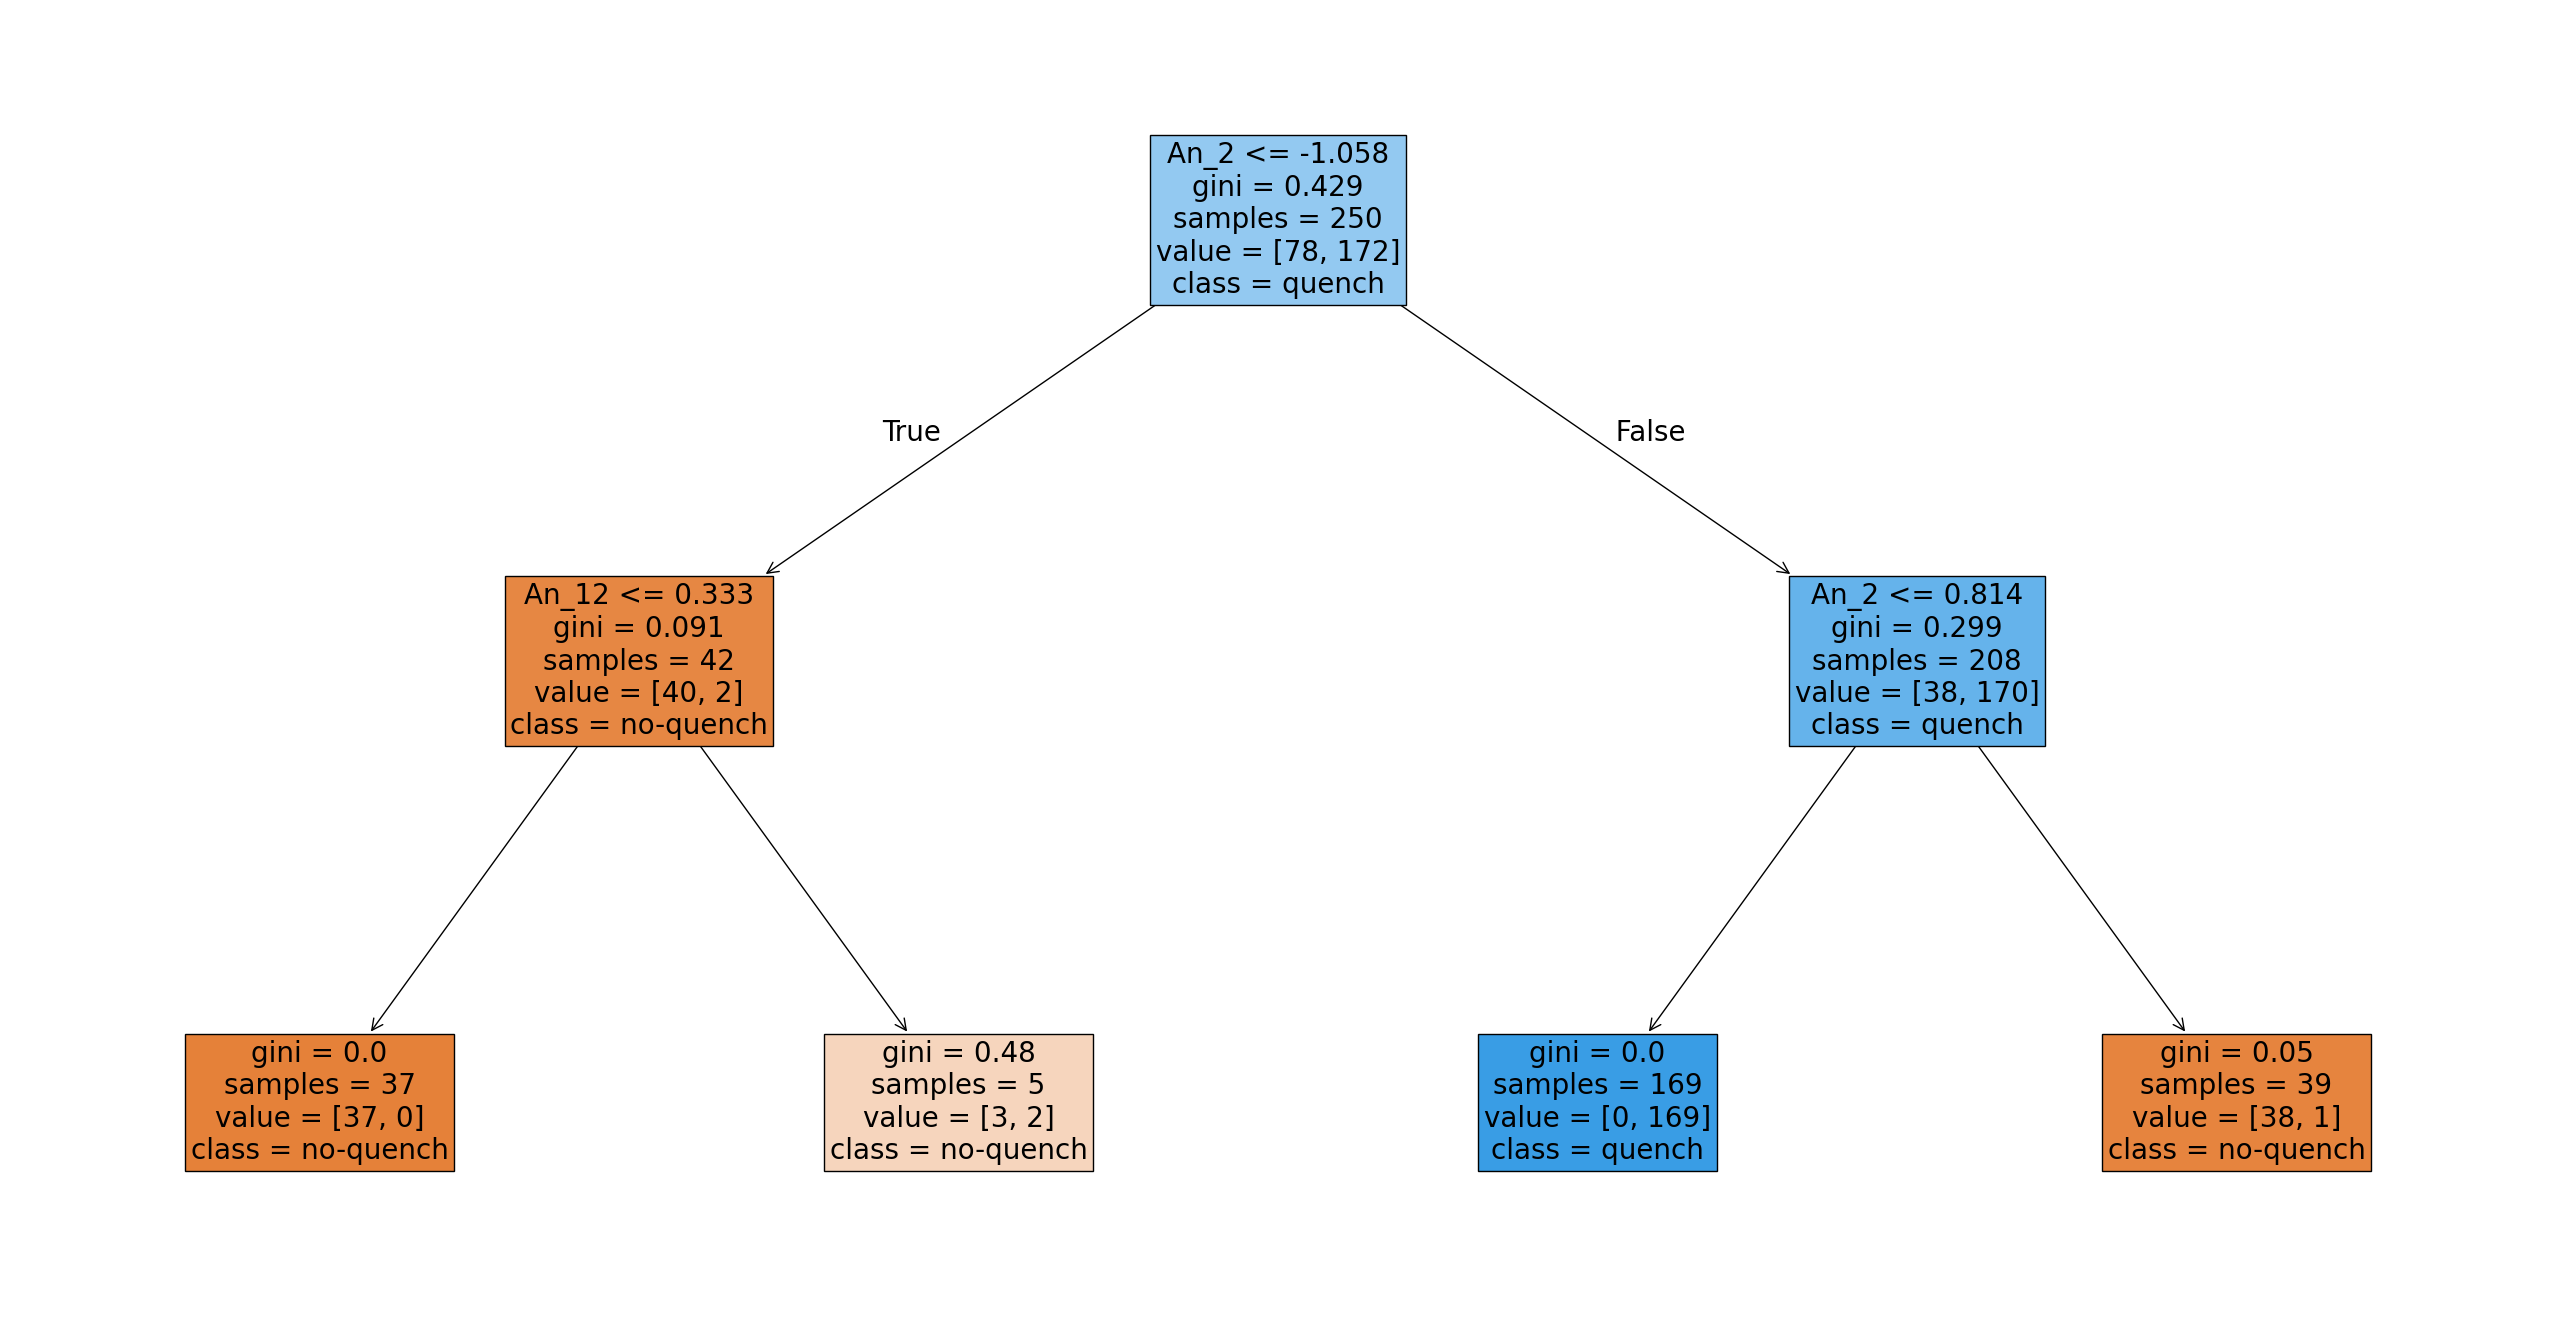
\includegraphics[width=\linewidth]{img/An_2_12_pt_dt.png}
	\caption{The structure of the tree built on harmonics $2, 12, 15$} \label{fig:dt-an-2-12-pt}
\end{figure}
All other \dts\ tested fell short of the model based on \an\ that was just described, in
\Cref{fig:best-dts} we can see a comparison of the best \dts\ built on every table, despite \cnmod\
having accuracy closer to the one obtained by the best model, it cannot recognize non-quench events
as effectively (the Irec score is lower).
\begin{figure}[t]
	\centering
	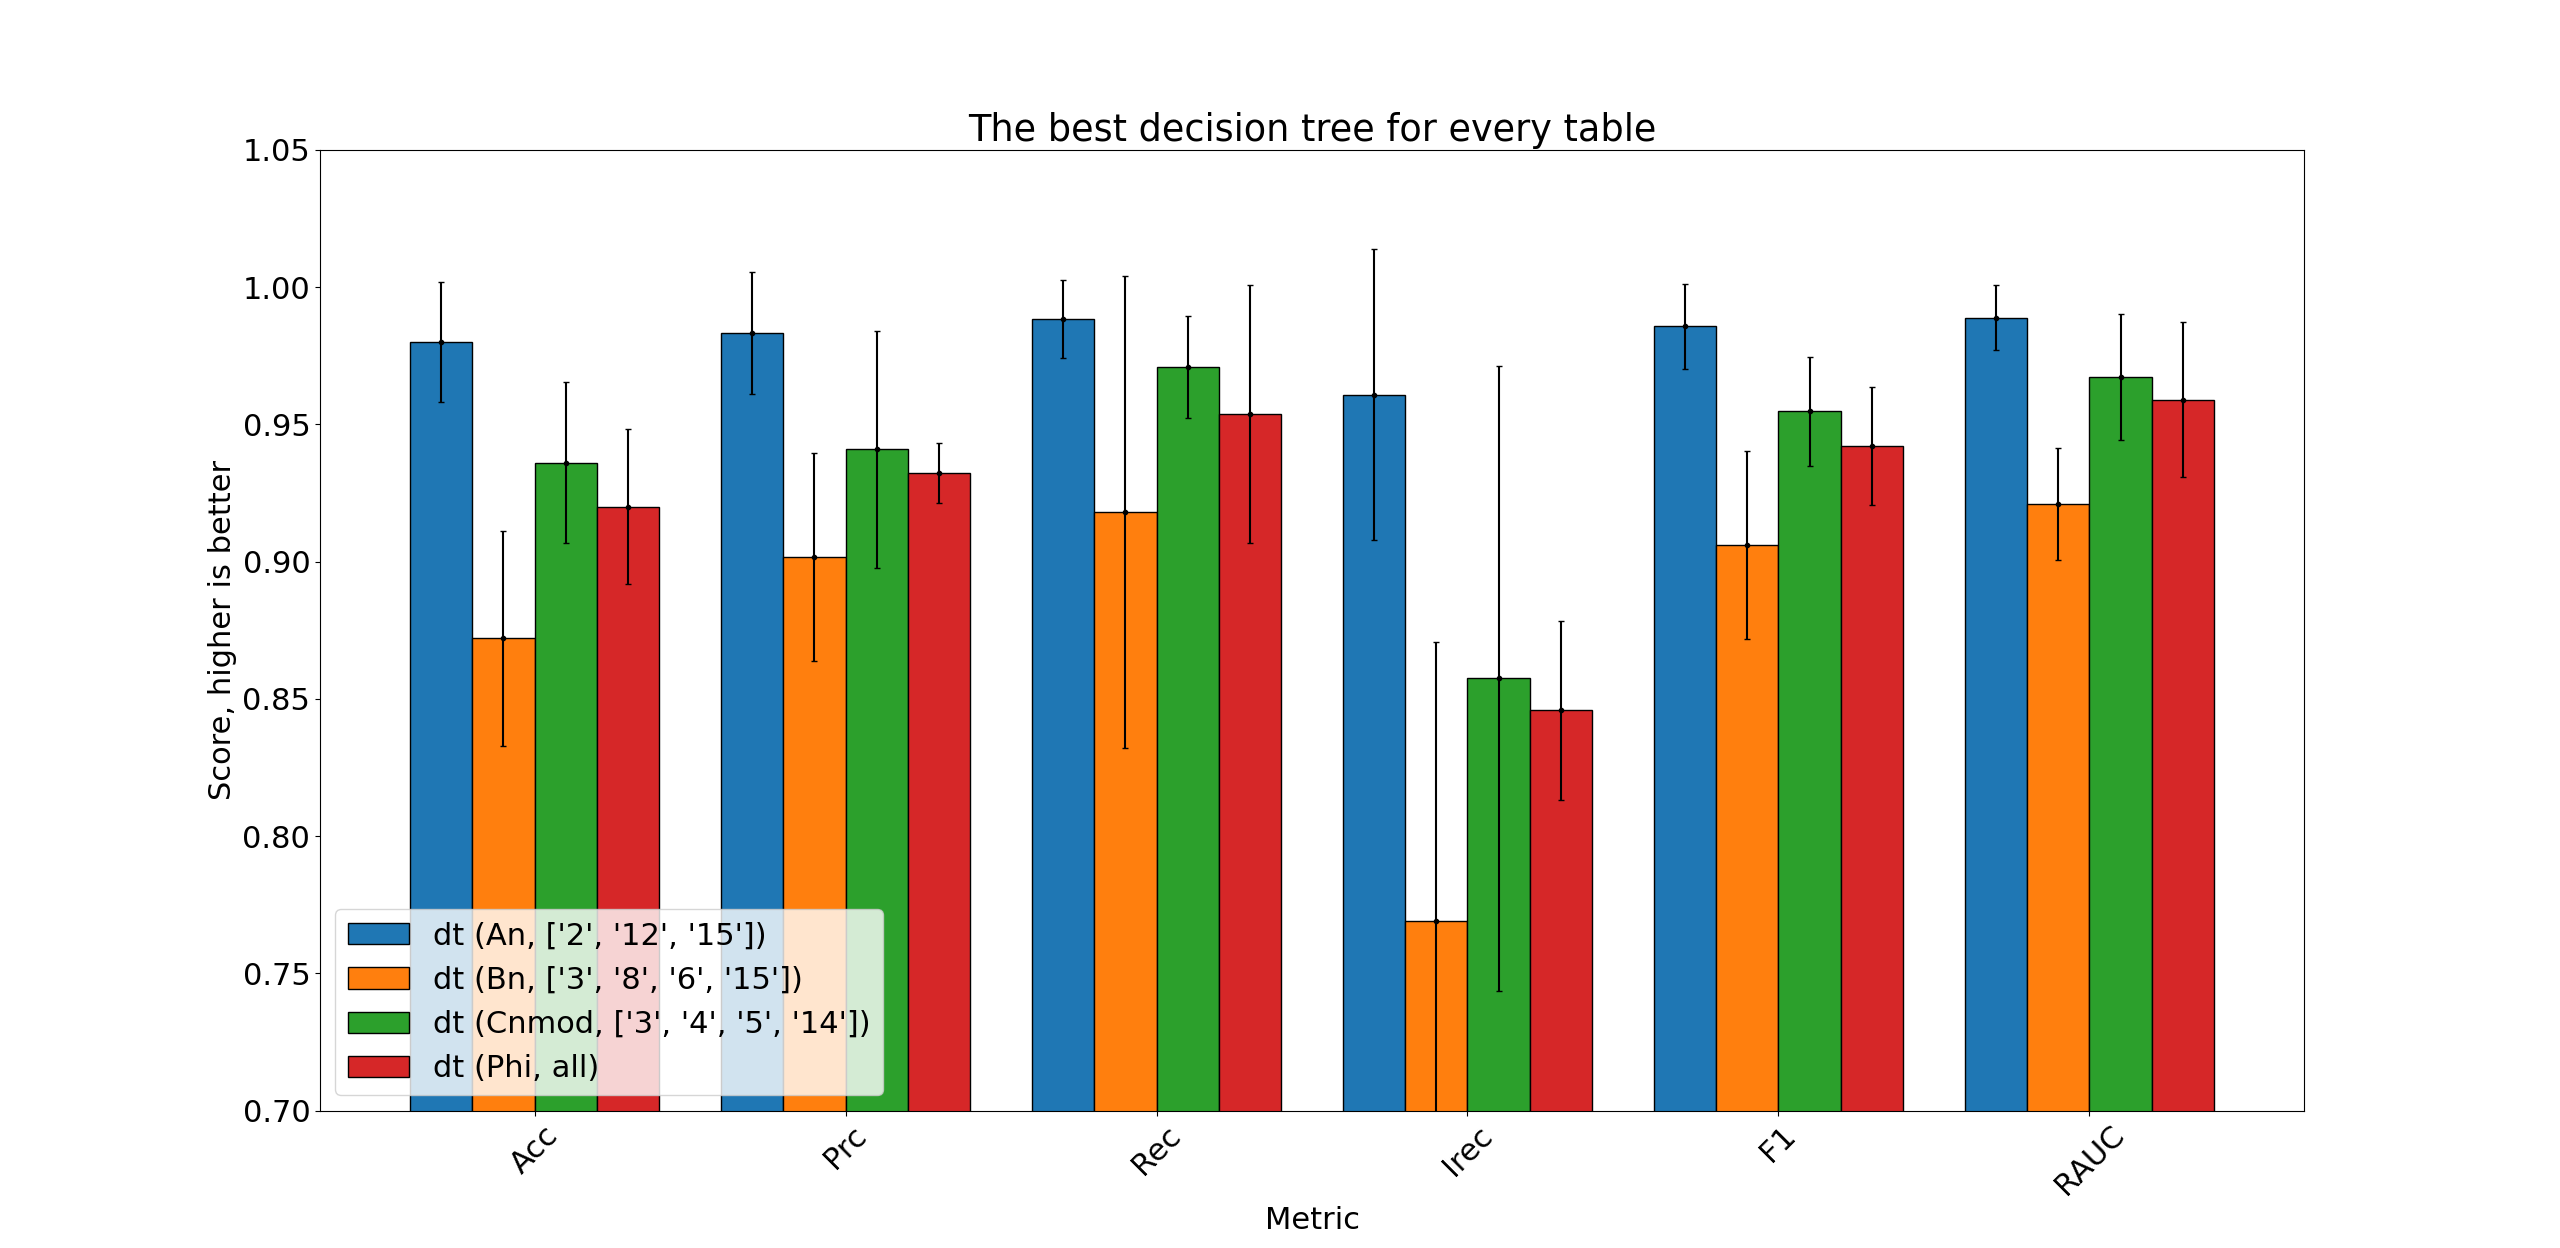
\includegraphics[width=\linewidth]{img/best_dts.png}
	\caption{Performance comparison of all the best decision trees} \label{fig:best-dts}
\end{figure}

\subsection{Random Forests}
\label{sec:qrp-rf}
As we said in \Cref{chp:ml} random forests (\rfs) use an ensemble of trees trained by bootstrap
sampling and perform splits on a random subset of features. As long as the trees are not too
complicated and the ensemble is not too big, \rfs\ are still quite easy to interpret, while
performing usually at least as good, if not better than the worst tree in the ensemble. Since they
are grouping \rfs\ can extrapolate information from complicated datasets containing different
sub-views (e.g., a dataset containing a subv-view for each of \an, \bn and \cnmod).

In most of our tests we considered \rfs\ trained on datasets built from one or more tables, each
table taken with the full harmonic content, we also did some tests on forests built on dataset
containing a subset of the available harmonics, just we did with trees. While the second approach
was more suitable for raw performance, the first one gave us insights, through the feature
importance metric, of which were the more important harmonics within the dataset.

Feature importance is a measure that we can use to understand which features are more prominent in
the \rf\ structure, this can give us an insight regarding what we should keep and what could be
probably taken away to achieve better performance. We analyzed the feature importance of \rfs\ built
on single views and then on an \rf\ constructed on the whole dataset, this is what we could conclude
from it:
\begin{itemize}
	\item The forest built on \an, performs most of the splits ($\approx 80\%$) using harmonic
	      number $2$.
	\item The forest built on \bn, performs most of the splits using a mix of different
	      harmonics, $2$ is not among the first $6$ for importance. Harmonics
	      $6, 9, 3, 14, 7$ and $5$ are the ones used the most to perform splits inside the
	      random forest.
	\item The forest built on \cnmod, uses harmonic number $2$ to perform over $50\%$ of the
	      splits, the rest are handled mainly by harmonics $5, 9$ and $13$.
	\item The forest built on \phin, uses many different harmonics to perform the splits (mainly
	      $10, 12, 6$ and $10$).
	\item If we train a forest on the whole dataset, we can see that $\approx90\%$ of the splits were computed by using harmonics $2$ and $3$ from \cnmod, and harmonics $12, 2$ and $14$ from \an.
\end{itemize}

In \Cref{fig:best-rfs} we plotted the metrics for the $4$ best performing random forests,
independently of the dataset they were trained on, the best model achieved accuracy of $\approx 98.8\%$, while the other models remain above $98\%$.
\todo{Cambiare il plot: toglierre il titolo, cambiare AUC con RAUC nelle metriche}
\begin{figure}
	\centering
	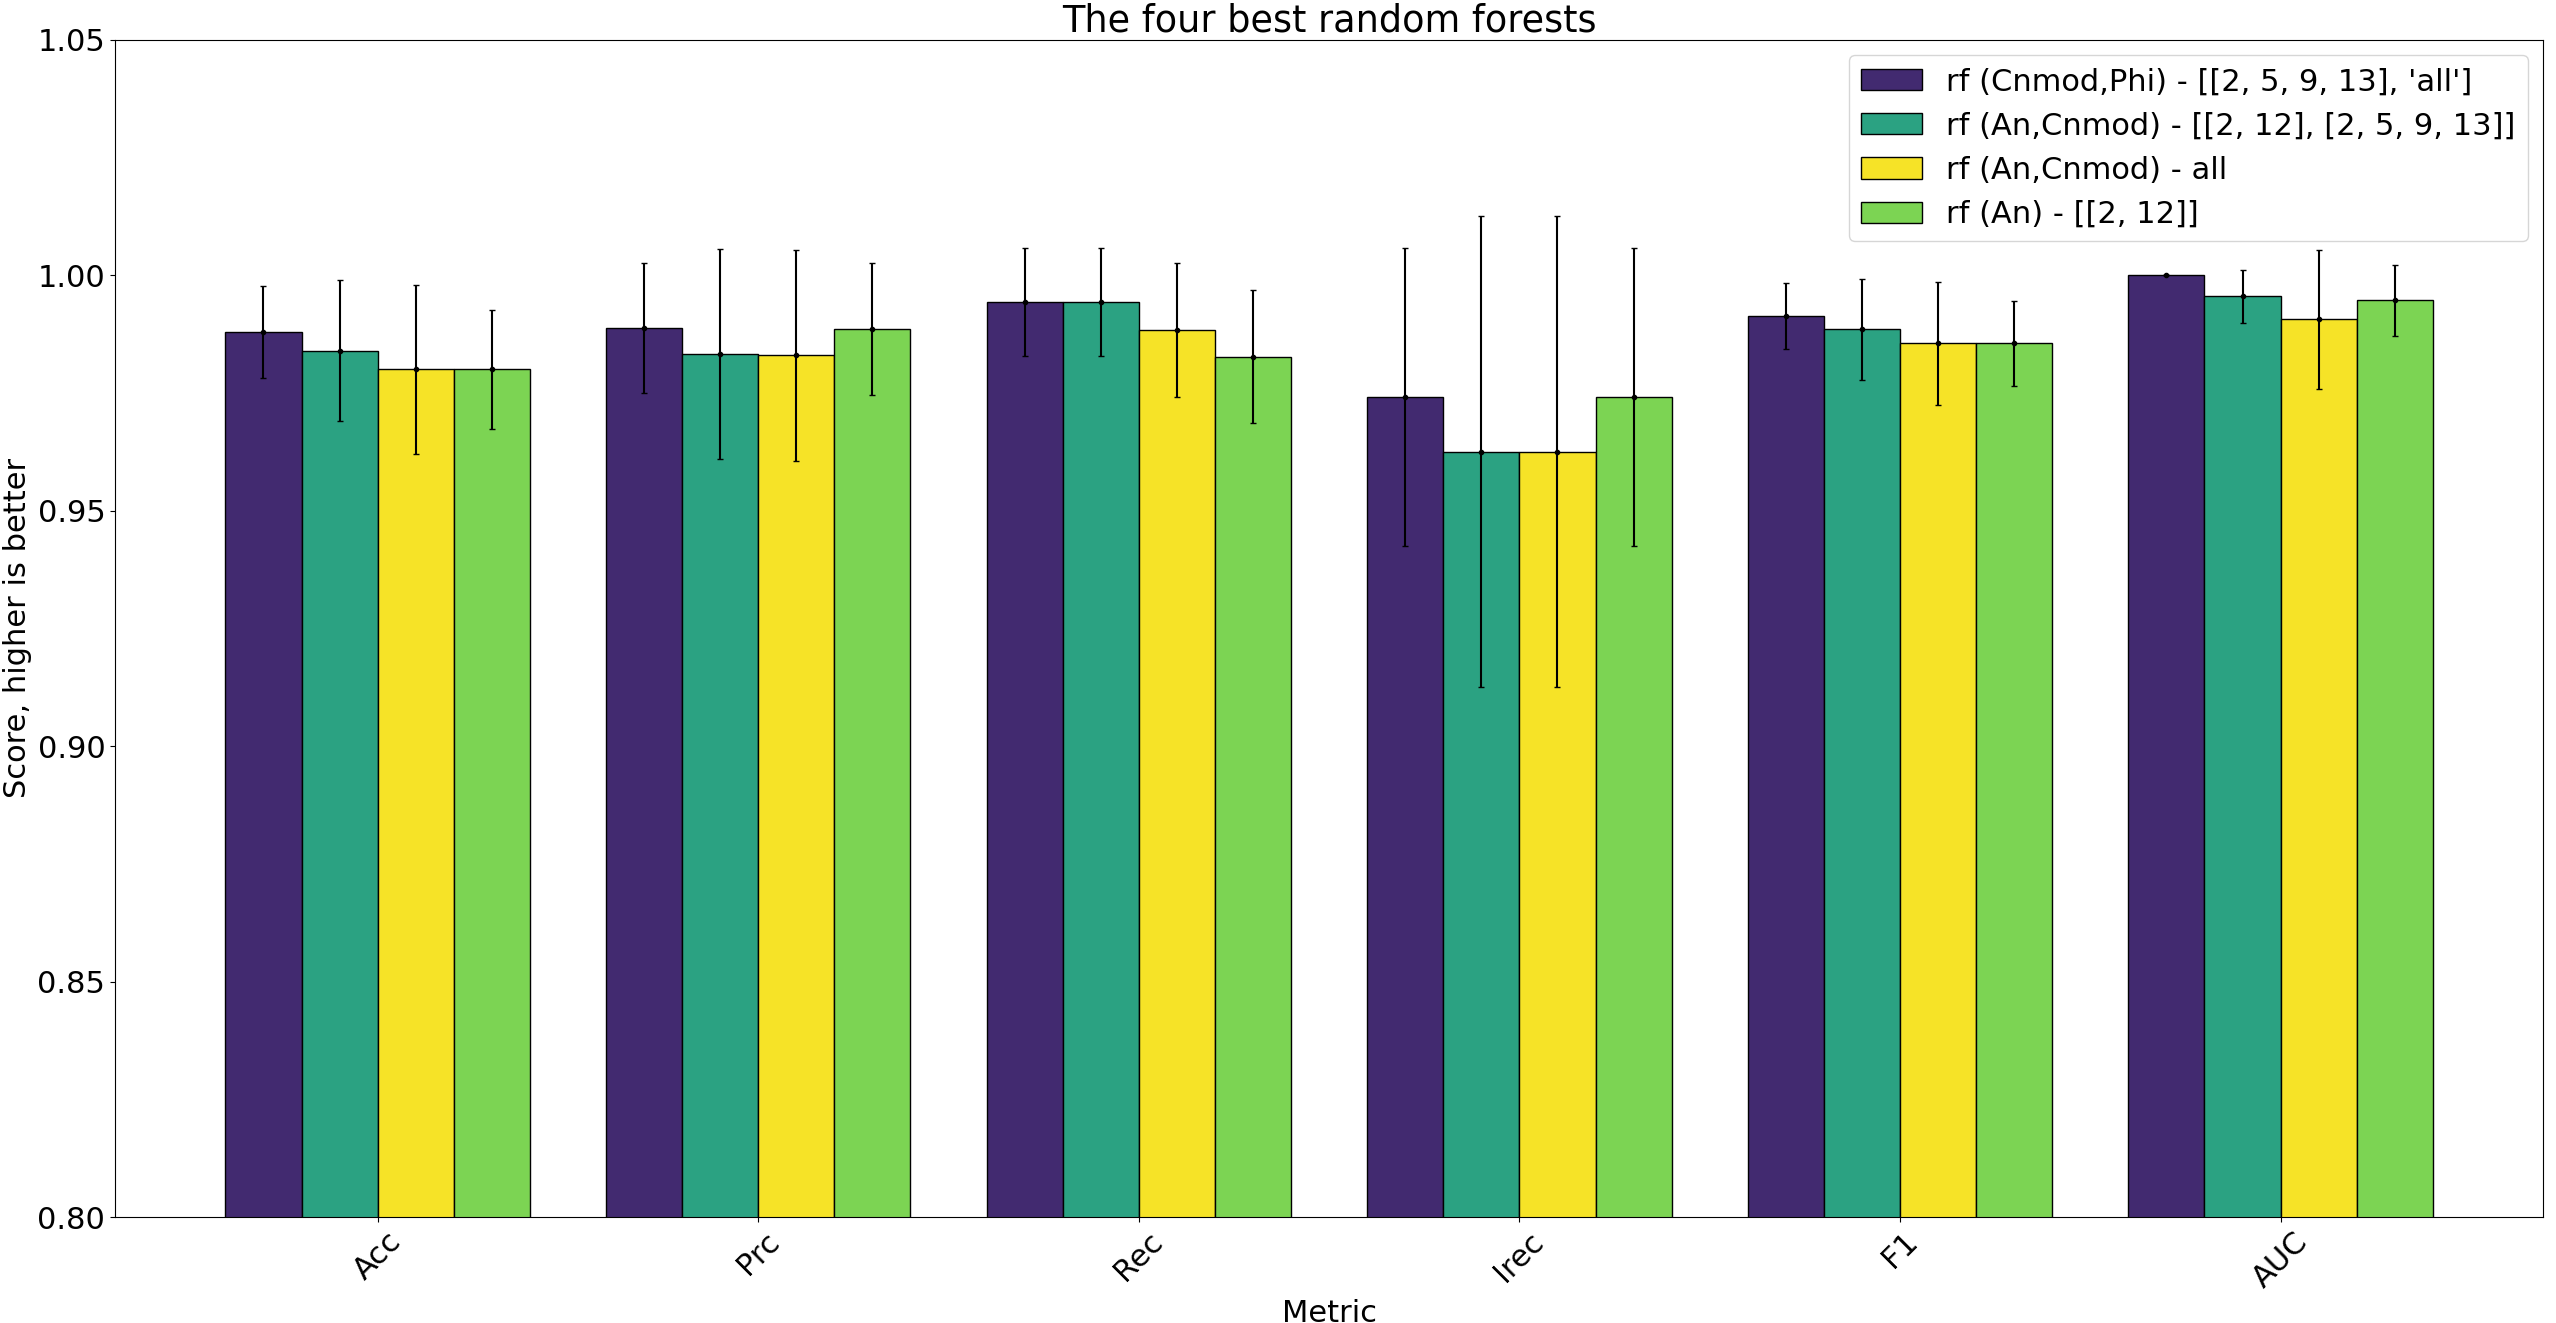
\includegraphics[width=\linewidth]{img/best_rfs.png}
	\caption{The best random forests} \label{fig:best-rfs}
\end{figure}
The performance for the best \rf\ \Cref{tbl:rf-cnmod-phi-perf} are definitely solid, and with some more work we could probably achieve better
results, since the models considered above are trained on datasets obtained by grouping
different sub-views\footnote{Which is very different from grouping trees trained on different
	sub-views.}, regardless of the correlation. We decided not to explore this solution more
since, as we will see briefly, \rfs\ can be more complicated to interpret than a model
we devised and will be introduced in a later section.
\begin{table}[t]
	\caption{Average and standard deviation of the performance for the best \rf\ over the outer \cv\
		folds.}\label{tbl:}

	\bigskip
	\setlength{\tabcolsep}{6pt}
	\centering
	\begin{tabular}{ccccccc}
		\toprule
		\textbf{}    & \textbf{Acc} & \textbf{Prc} & \textbf{Rec} & \textbf{Irec} & \textbf{F1} & \textbf{RAUC} \\
		\midrule
		Mean         & 0.988        & 0.989        & 0.994        & 0.974         & 0.991
		             & 1.0                                                                                      \\
		\textsc{std} & 0.010        & 0.013        & 0.011        & 0.032         & 0.007
		             & 0.0                                                                                      \\
		\bottomrule
	\end{tabular}
\end{table}
%{'accuracy-mean': np.float64(0.9879999999999999), 'accuracy-std': np.float64(0.009797958971132722), 'precision-mean': np.float64(0.9887301587301588), 'precision-std': np.float64(0.01380496184454534), 'recall-mean': np.float64(0.9942857142857143), 'recall-std': np.float64(0.011428571428571432), 'inv-recall-mean': np.float64(0.9741666666666667), 'inv-recall-std': np.float64(0.03166666666666666), 'f1-mean': np.float64(0.991385997142274), 'f1-std': np.float64(0.0070348834762717265), 'roc_auc-mean': np.float64(1.0), 'roc_auc-std': np.float64(0.0)}

To conclude this section we analyze the structure of the best \rf\ previously found and we
check the performance obtained on the blind-test set. The best \rf\ contains $5$ trees, each tree
has a maximum depth of $4$ and the number of internal nodes and leaves is always quite limited (on
average the trees inside the forest contain $4$ internal nodes). The most important harmonics are
$2$ and $5$, taken from \cnmod, and $6$ and $10$, taken from \phin. If we test the model on the
blind-test set \db, we see that the model only makes one classification error among the $29$
samples, specifically a false positive.
\begin{table}[!ht]
	\caption{Performances of the best \rf\ on the blind test set $\mathscr
			D_\mathrm{test}$.}\label{tab:qrp-rf-test}

	\bigskip
	\setlength{\tabcolsep}{6pt}
	\centering
	\begin{tabular}{cccccc}
		\toprule
		\textbf{Acc} & \textbf{Prc} & \textbf{Rec} & \textbf{F1} & \textbf{Irec} & \textbf{RAUC} \\
		\midrule
		0.965        & 0.952        & 1            & 0.976       & 0.889         & 0.944         \\
		\bottomrule
	\end{tabular}
\end{table}

Before exploring the performance of the \rf\ alternative we will have a small digression dedicated
to the benchmarking model, \svcs.

\subsection{\svc}
A binary Support Vector Classifier (SVC), is a different declination of the \svm\ model, introduced
in \Cref{chp:ml}, and considers each sample as a vector in the Euclidean space, and finds a decision surface separating the vectors corresponding to two classes. This is achieved by maximizing the so-called \emph{margin}, intended as the minimal distance between the decision surface and the data images through a nonlinear mapping. The related optimization process exploits the so-called \emph{kernel trick} to automatically select this mapping within some prefixed families.

This model is meant to have very high performance at the expense of its explainability property,
that is why we chose it as our benchmarking model.

In the following we will be showing two different techniques, still based on trees, which yielded
very high performance and we will later close the chapter with an analysis of the model that we
chose to solve the problem performed the best overall.


\subsection{Tree Aggregators}
\label{sec:qrp-ta}
The best random forest is obtained by training the model on \an\ and \cnmod, the maximum depth of
its trees is $4$ and, while the maximum number of internal nodes is $5$, the majority of the
estimators contain only $4$ internal nodes. The most important harmonics in the structure are $2$ and $5$, for \cnmod, $6$ and $10$ for \phin.

While this \rf\ has a relatively simple structure, as we anticipated at the end of last section, we
can still do better.

Since many of the \dts\ generated in previous phases of testing have all been serialized, and we
know how well they perform from the analysis of the performance obtained in the external \cv\
procedure, we can create an ensemble of the best tree for every table, and then we can aggregate the
performance by doing majority voting.

To test the performance of such models, which we called Tree Aggregators (\tas), to differenciate them from
\rfs, we first aggregated the best decision tree for every table, then we retrained the
models on the reduced dataset using a $5$-fold \cv, and finally we aggregate all the predictions via
majority voting. To avoid defining a procedure to break ties, in the following, we will be
presenting the performance obtained by training \tas\ on triplets (e.g., \an, \bn, \cnmod).

We remark that the retraining procedure was necessary since \dts\ are stored after a full retrain on
the reduced dataset (the $250$ samples at our disposal). This choice forces us to repeat a
training procedure whenever we want to test the performance of models in different configurations,
since the only non-used data available to us are the ones stored in the safe, which was not used
until the last possible minute to avoid biased model choices.

We constructed \tas\ by aggregating three sub-views of the original dataset, and we benchmarked it
against \rfs\ trained on the best performing sub-view for each triplet and \svcs trained on full views (therefore
containing the harmonics). As we can see in \Cref{fig:triplets-performance}, \tas\ usually perform
closer to \svcs\ than \rfs, with the exception of the RAUC score, which predilects \rfs\,
performance for the best \ta\ among the $4$ benchmarked in \Cref{fig:triplets-performance} are
indicated in \Cref{tbl:an-bn-cnmod-ta-perf}.
\begin{figure}[!h]
	\centering
	\begin{subfigure}{0.49\linewidth}
		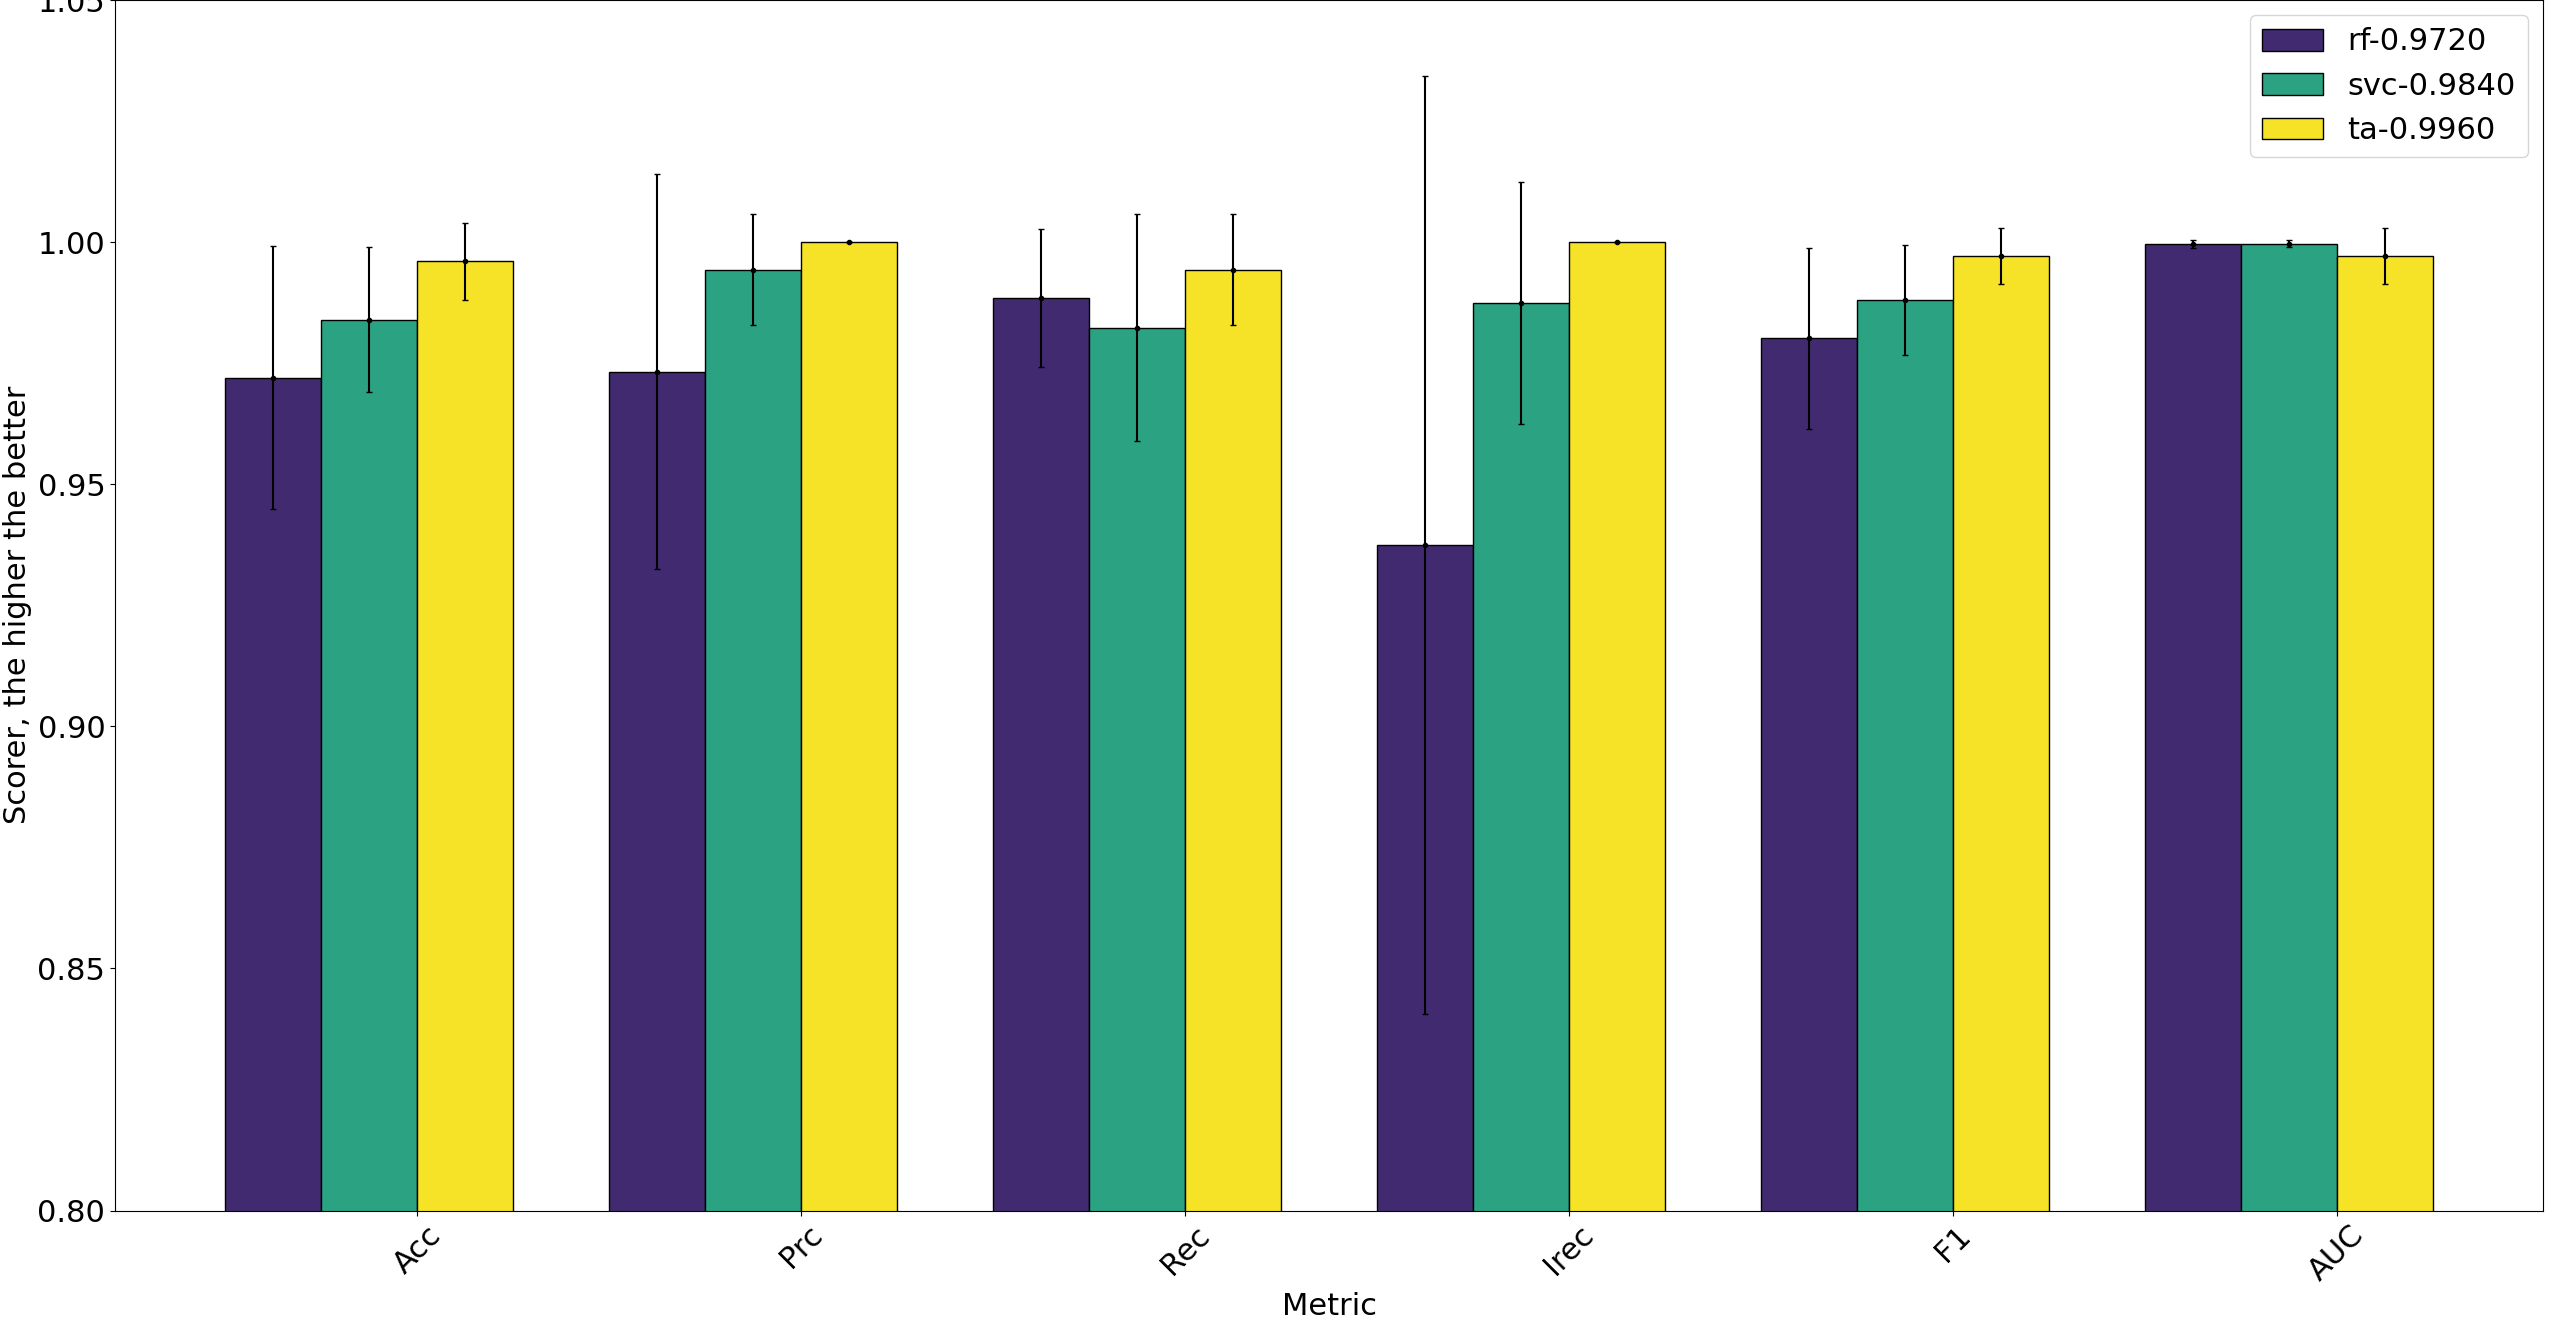
\includegraphics[width=\linewidth]{img/An_Bn_Cnmod_ta.png}
		\subcaption{\an, \bn, \cnmod}
	\end{subfigure}
	\begin{subfigure}{0.49\linewidth}
		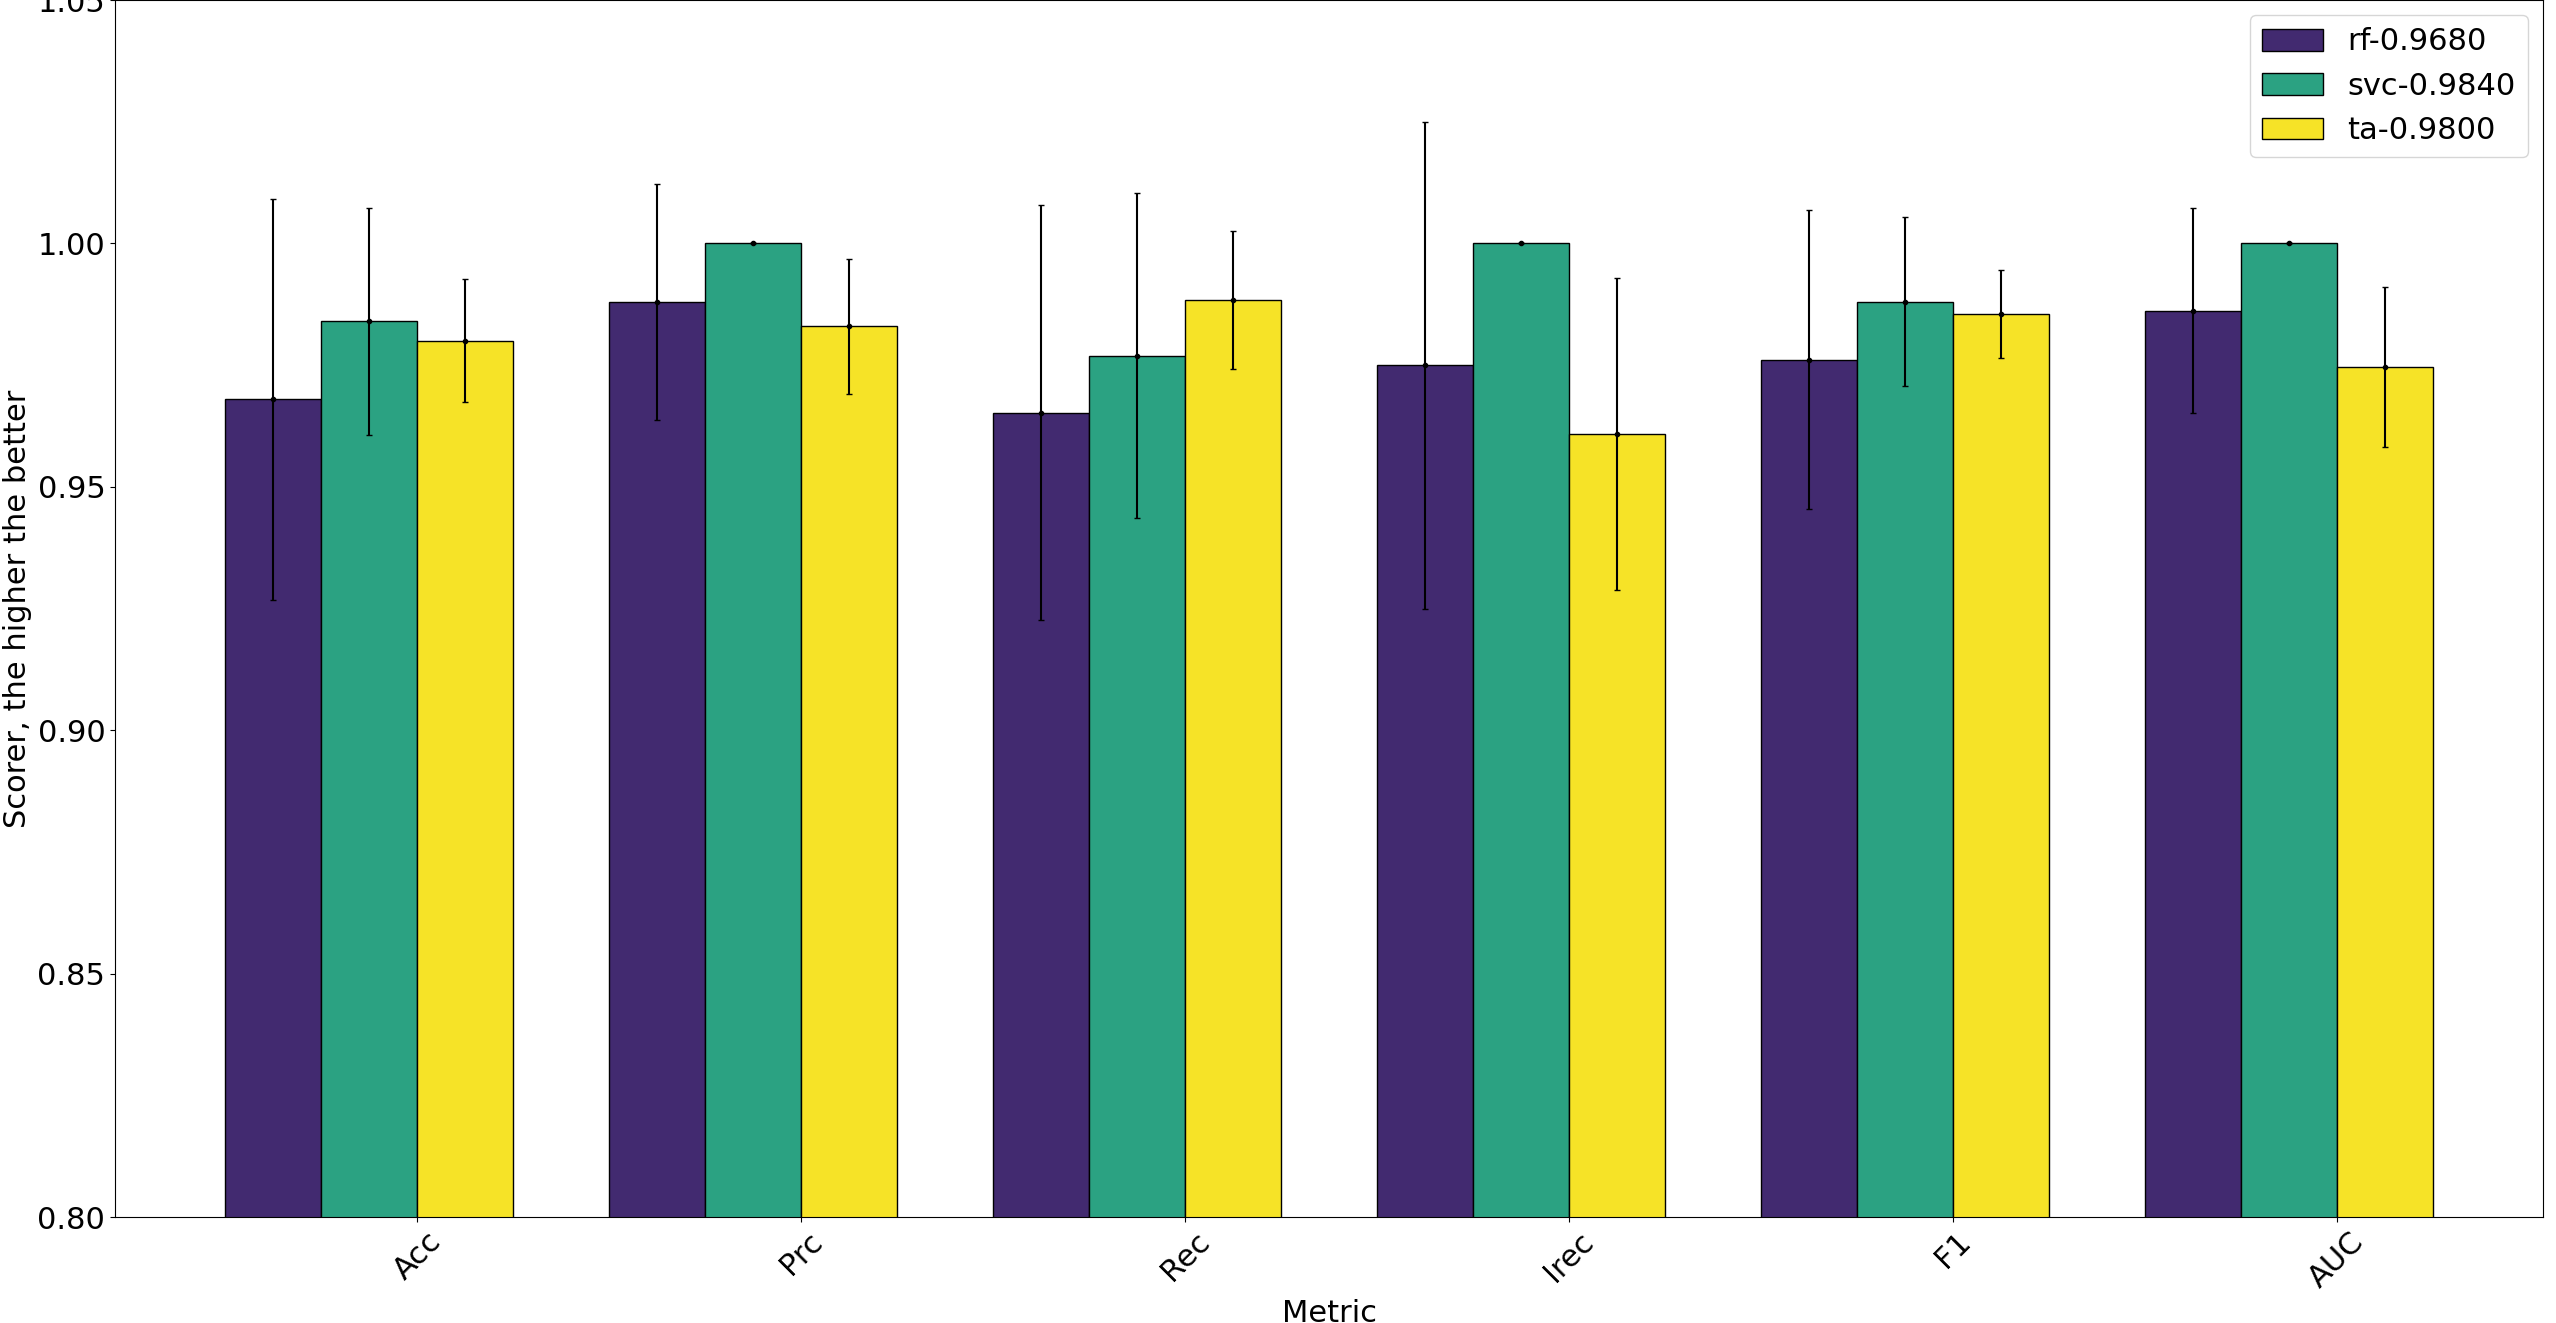
\includegraphics[width=\linewidth]{img/An_Bn_Phi_ta.png}
		\subcaption{\an, \bn, \phin}
	\end{subfigure}
	\begin{subfigure}{0.49\linewidth}
		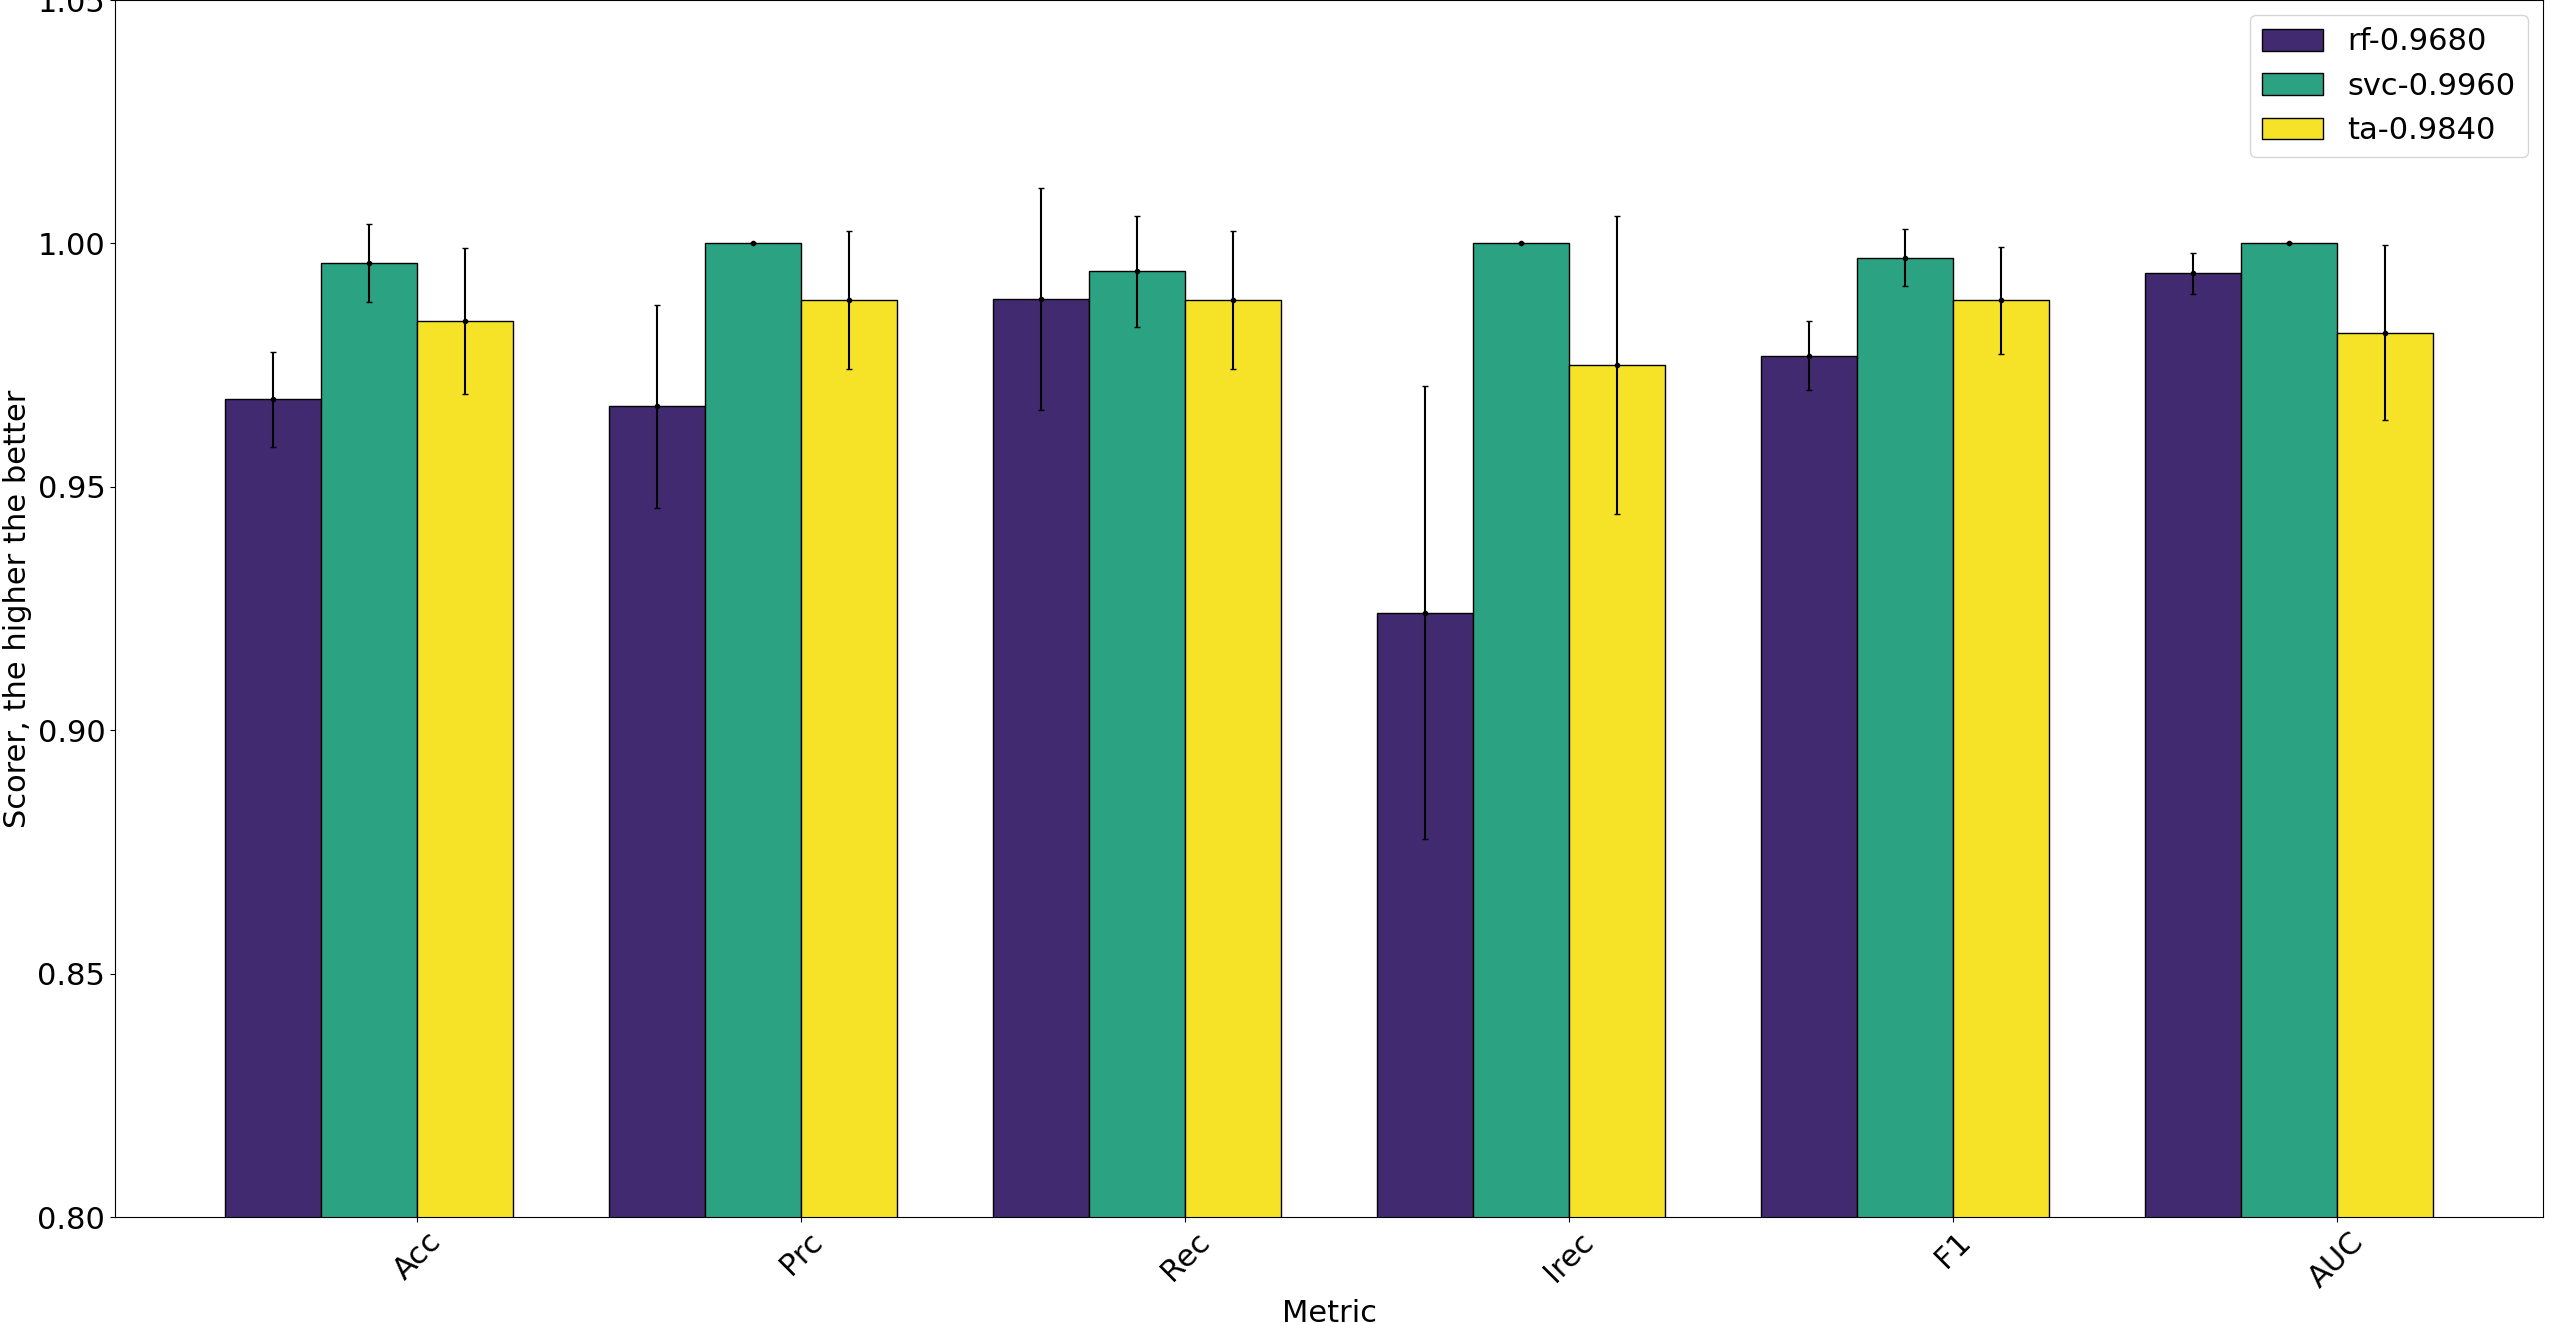
\includegraphics[width=\linewidth]{img/An_Cnmod_Phi_ta.png}
		\subcaption{\an, \cnmod, \phin}
	\end{subfigure}
	\begin{subfigure}{0.49\linewidth}
		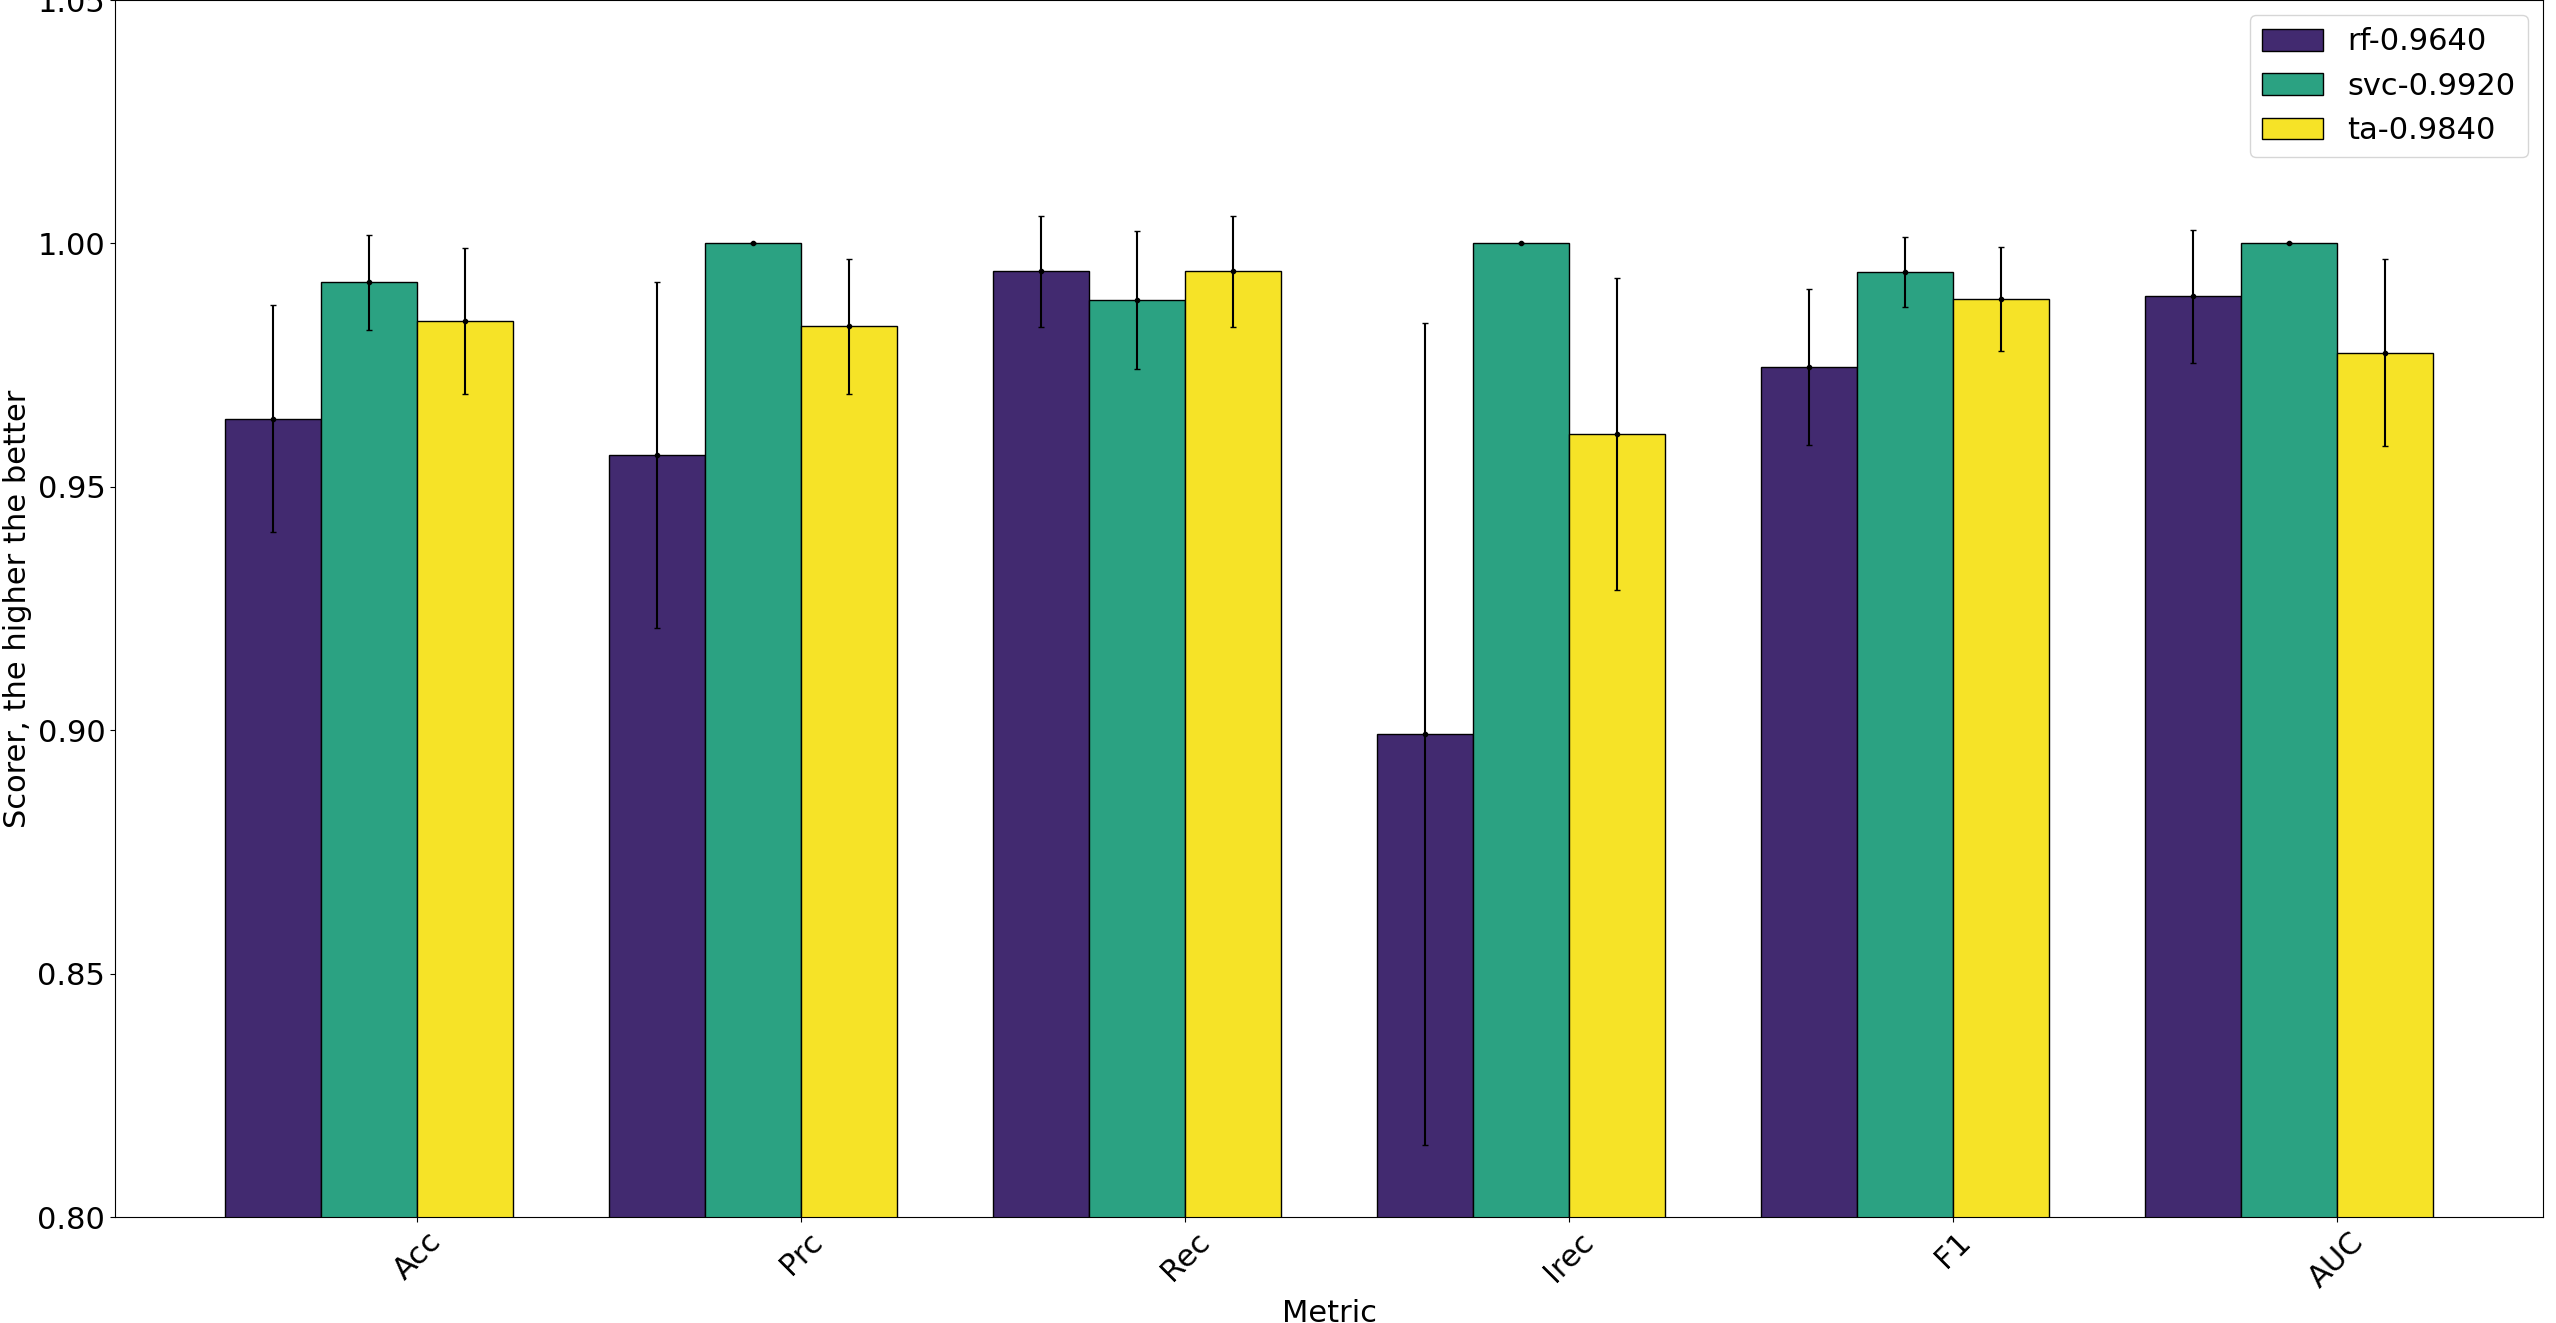
\includegraphics[width=\linewidth]{img/Bn_Cnmod_Phi_ta.png}
		\subcaption{\bn, \cnmod, \phin}
	\end{subfigure}
	\caption{Performance of \tas\ benchmarked against \rfs\ and \svcs, each model was trained on
		the same triplet to have an even testing ground.} \label{fig:triplets-performance}
\end{figure}
\begin{table}[!h]
	\caption{Average and standard deviation of the \ta\ trained on sub-views of \an, \bn and
		\cnmod.}\label{tbl:an-bn-cnmod-ta-perf}

	\bigskip
	\setlength{\tabcolsep}{6pt}
	\centering
	\begin{tabular}{ccccccc}
		\toprule
		\textbf{}    & \textbf{Acc} & \textbf{Prc} & \textbf{Rec} & \textbf{Irec} & \textbf{F1} & \textbf{RAUC} \\
		\midrule
		Mean         & 0.996        & 1.0          & 0.994        & 1.0           & 0.997
		             & 0.997                                                                                    \\
		\textsc{std} & 0.008        & 0.0          & 0.011        & 0.0           & 0.006
		             & 0.006                                                                                    \\
		\bottomrule
	\end{tabular}
\end{table}
%Final scores for the model:
%accuracy -- avg: 0.9960   std: 0.0080
%precision -- avg: 1.0000   std: 0.0000
%recall -- avg: 0.9943   std: 0.0114
%inv-recall -- avg: 1.0000   std: 0.0000
%f1 -- avg: 0.9971   std: 0.0058
%roc_auc -- avg: 0.9971   std: 0.0057


We tested the performance of the \ta\ model using a different subview for \cnmod, which performed
better as a tree, but it yielded worse performance when put in the \ta\ ensemble. For further
testing, we picked the best \ta\ (the one built on \an, \bn\ and \cnmod) and we compared its
performance against the best \svc\ and the best \rf, which were described in the respective
sections. The result is shown in \Cref{fig:ta-rf-svc-comparison}, the performance of the \rf\ are
always at most on par with the performance obtained by the \ta and the \svc. The only case in which
the \rf\ is ever so slightly better than the \ta, is the ROC-AUC score.

Since both \ta\ and \rf\ predictions are aggregated via majority voting we could address this odd
behavior by considering that the number of trees contained in the \rf\ is larger than the number of
trees contained in the \ta\ therefore decisions could be more biased: in the first case we need
three estimators to obtain majority, while in the latter we only need two.
\begin{figure}[!h]
	\centering
	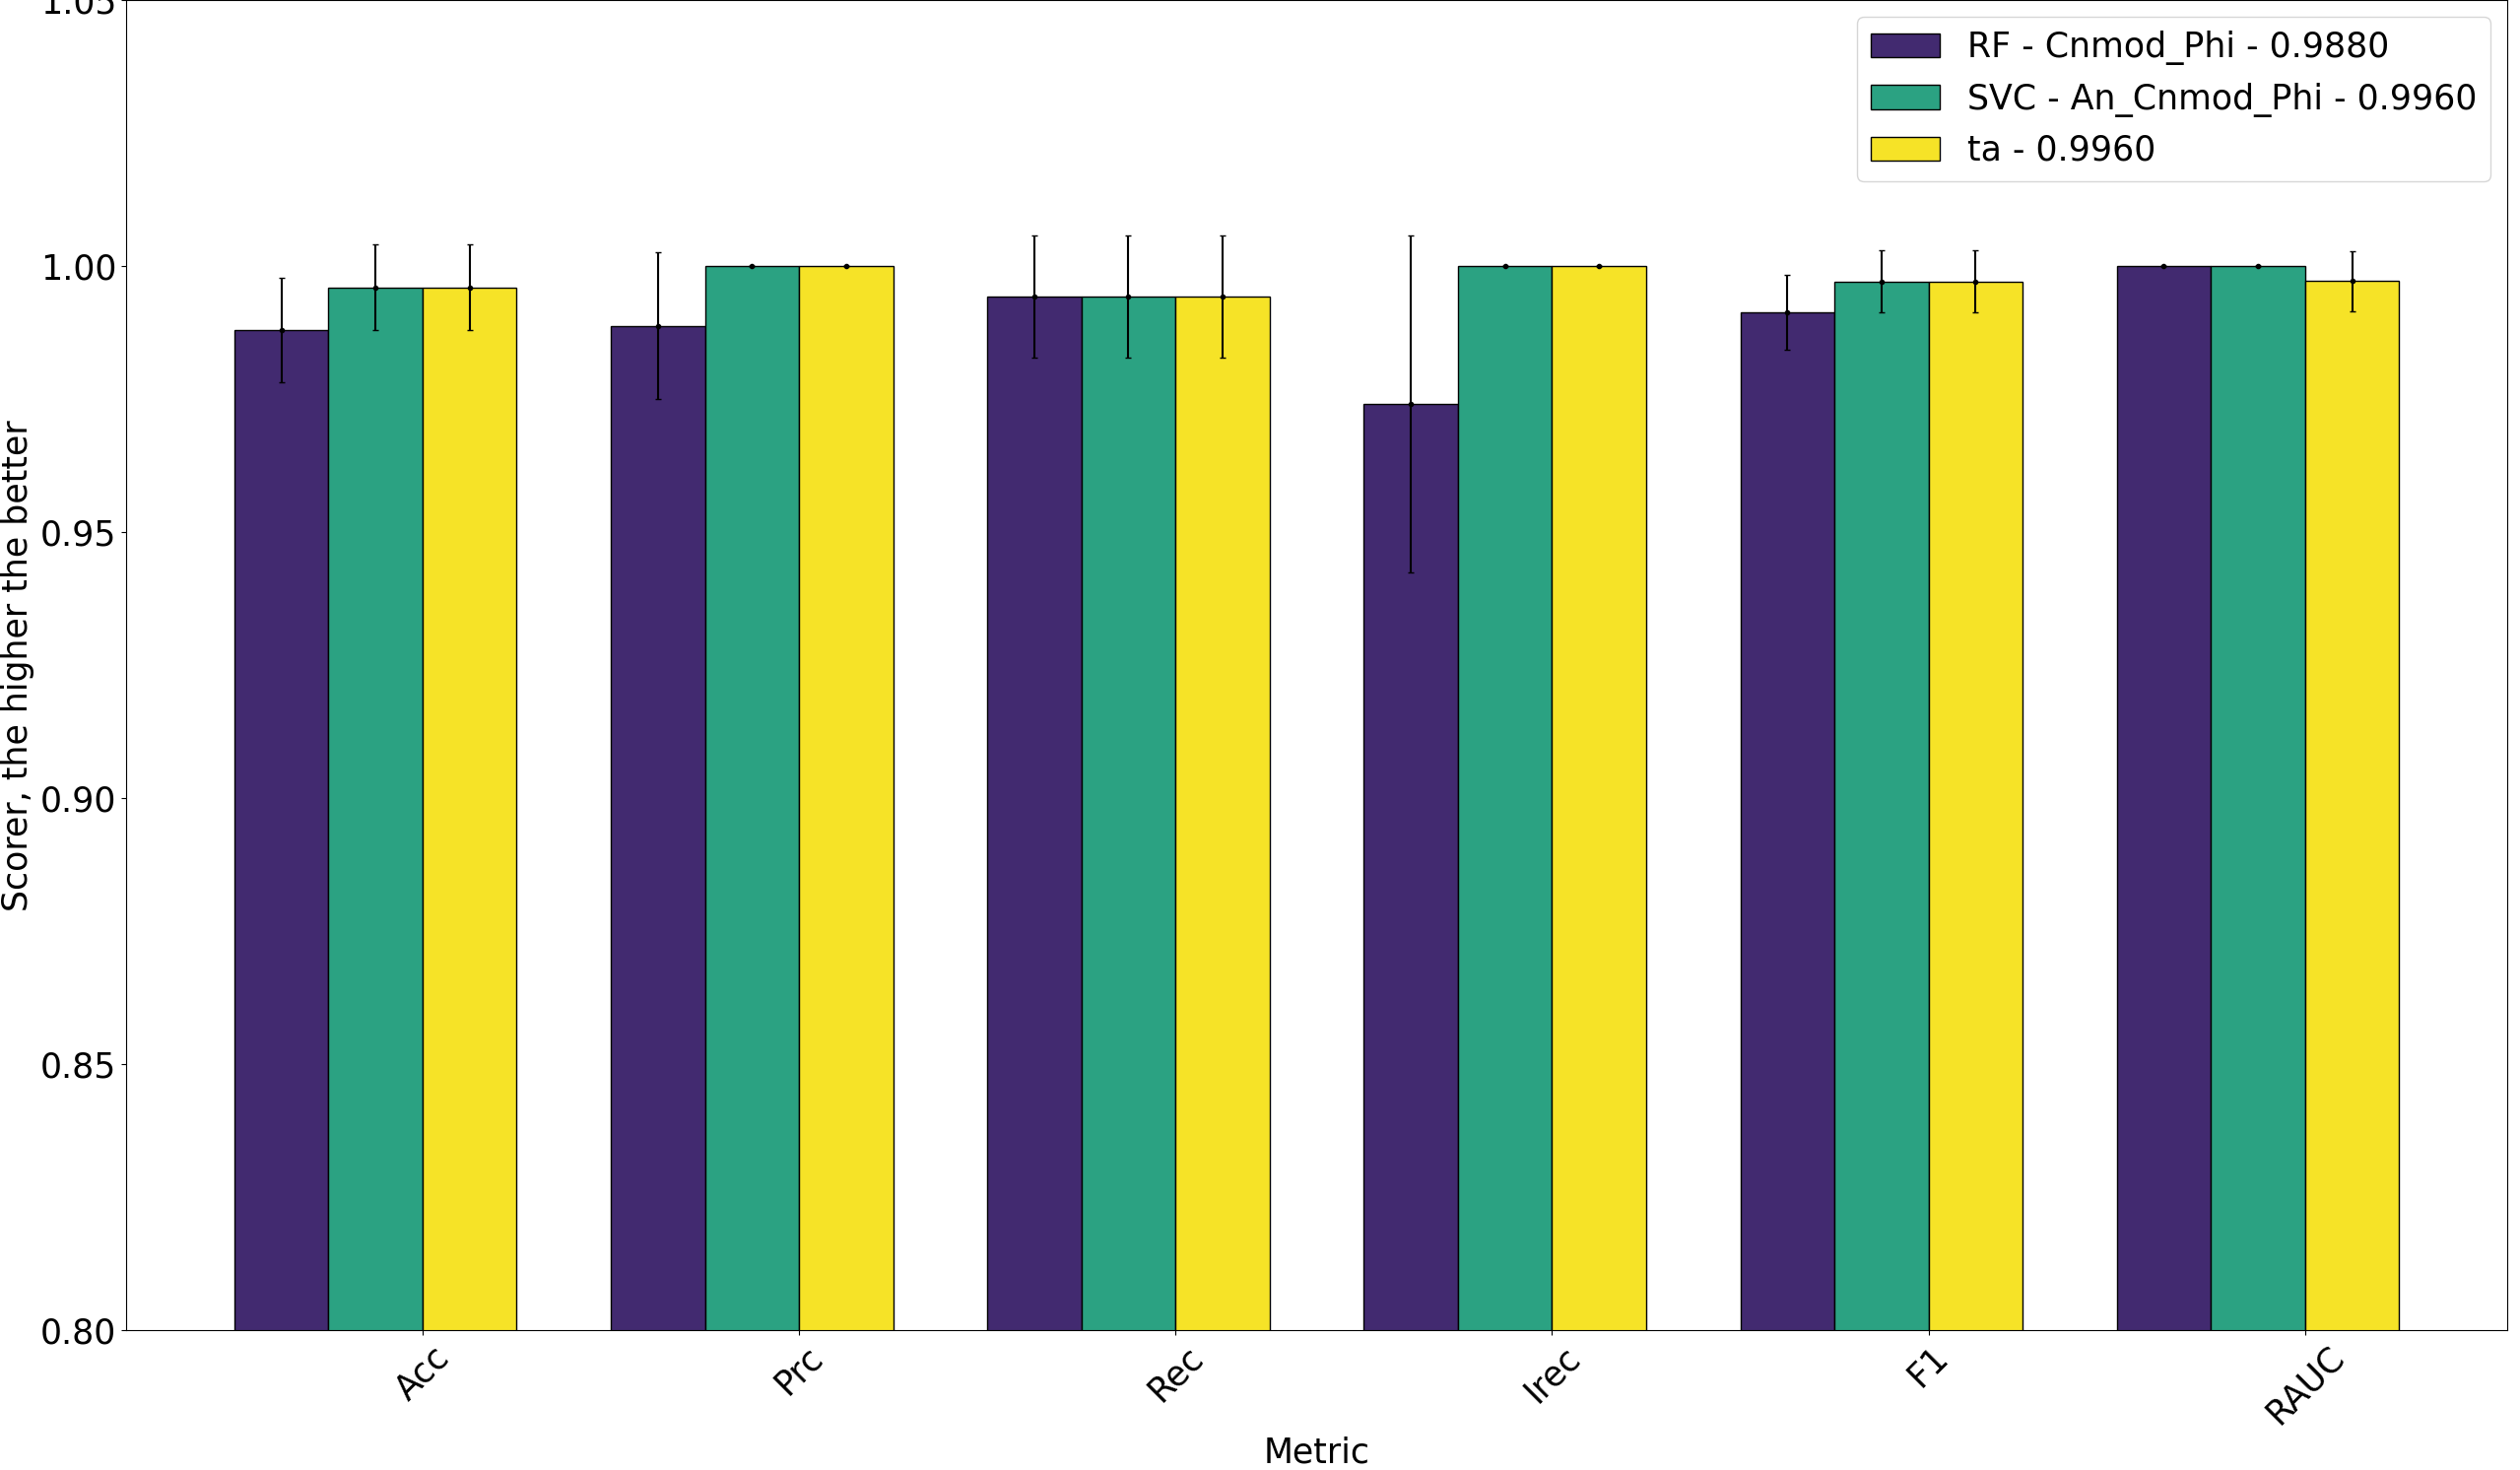
\includegraphics[width=\linewidth]{img/best_rf_ta_svc_compared.png}
	\caption{A performance comparison between the best \rf, the best \svc, and the best \ta,
		each of them trained on the sub-view of the original datasets the yields the best possible
		performance} \label{fig:ta-rf-svc-comparison}
\end{figure}

To close this section we will be analyzing the \ta\ constructed on \an, \bn\ and \cnmod providing a
description of the trees contained in the model and we will compute the performance metrics on the
blind-test set (\db). This model contains
$3$ trees: The one built on a sub-view of \an\ is shown in \Cref{fig:dt-an-2-12-pt}, the
other two, one built on \bn, and one built on \cnmod, are shown in \Cref{fig:part-of-bta}. Compared
to the trees we described at the end of the end of \Cref{sec:qrp-rf} we have trees which are a bit
more complex: having depth between $4$ and $5$, which we still consdier very reasonable, having a
larger volume of both internal nodes and leaves.

\begin{figure}[!ht]
	\centering
	\begin{subfigure}{\linewidth}
		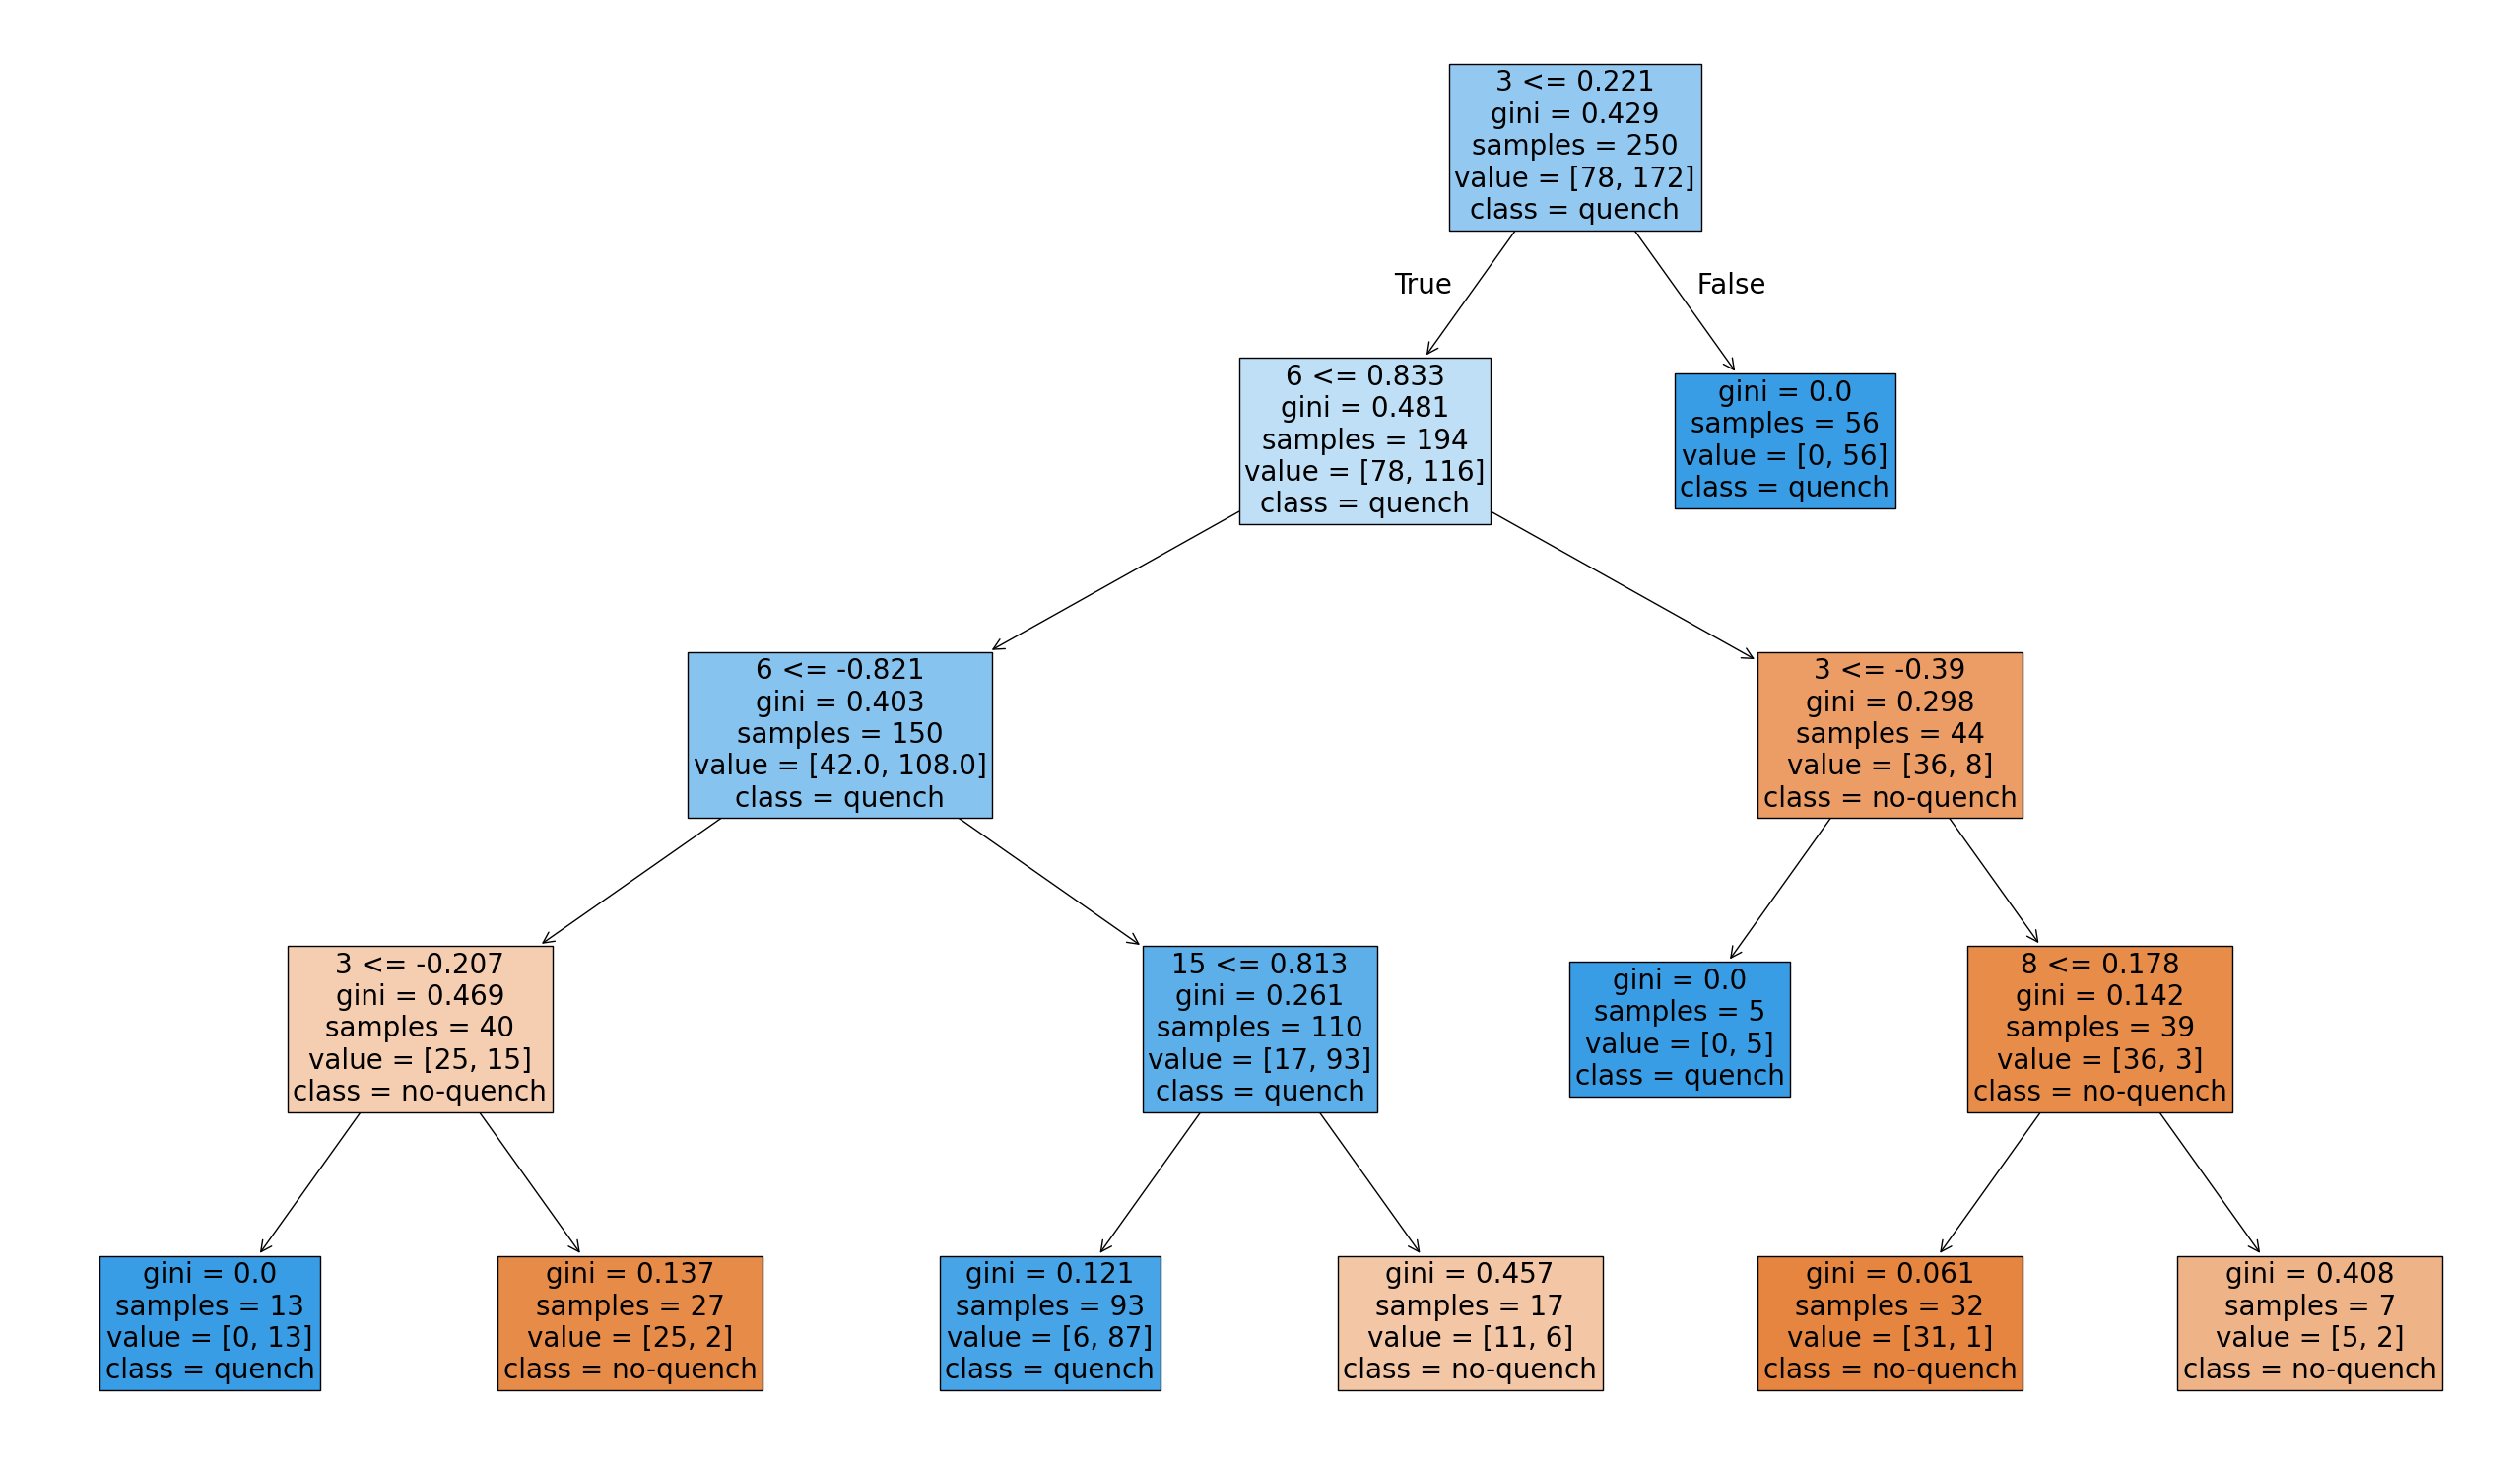
\includegraphics[width=\linewidth]{img/Bn_3_6_8_15_pt_dt.png}
		\subcaption{Tree trained on a subview of \bn}
	\end{subfigure}
	\begin{subfigure}{\linewidth}
		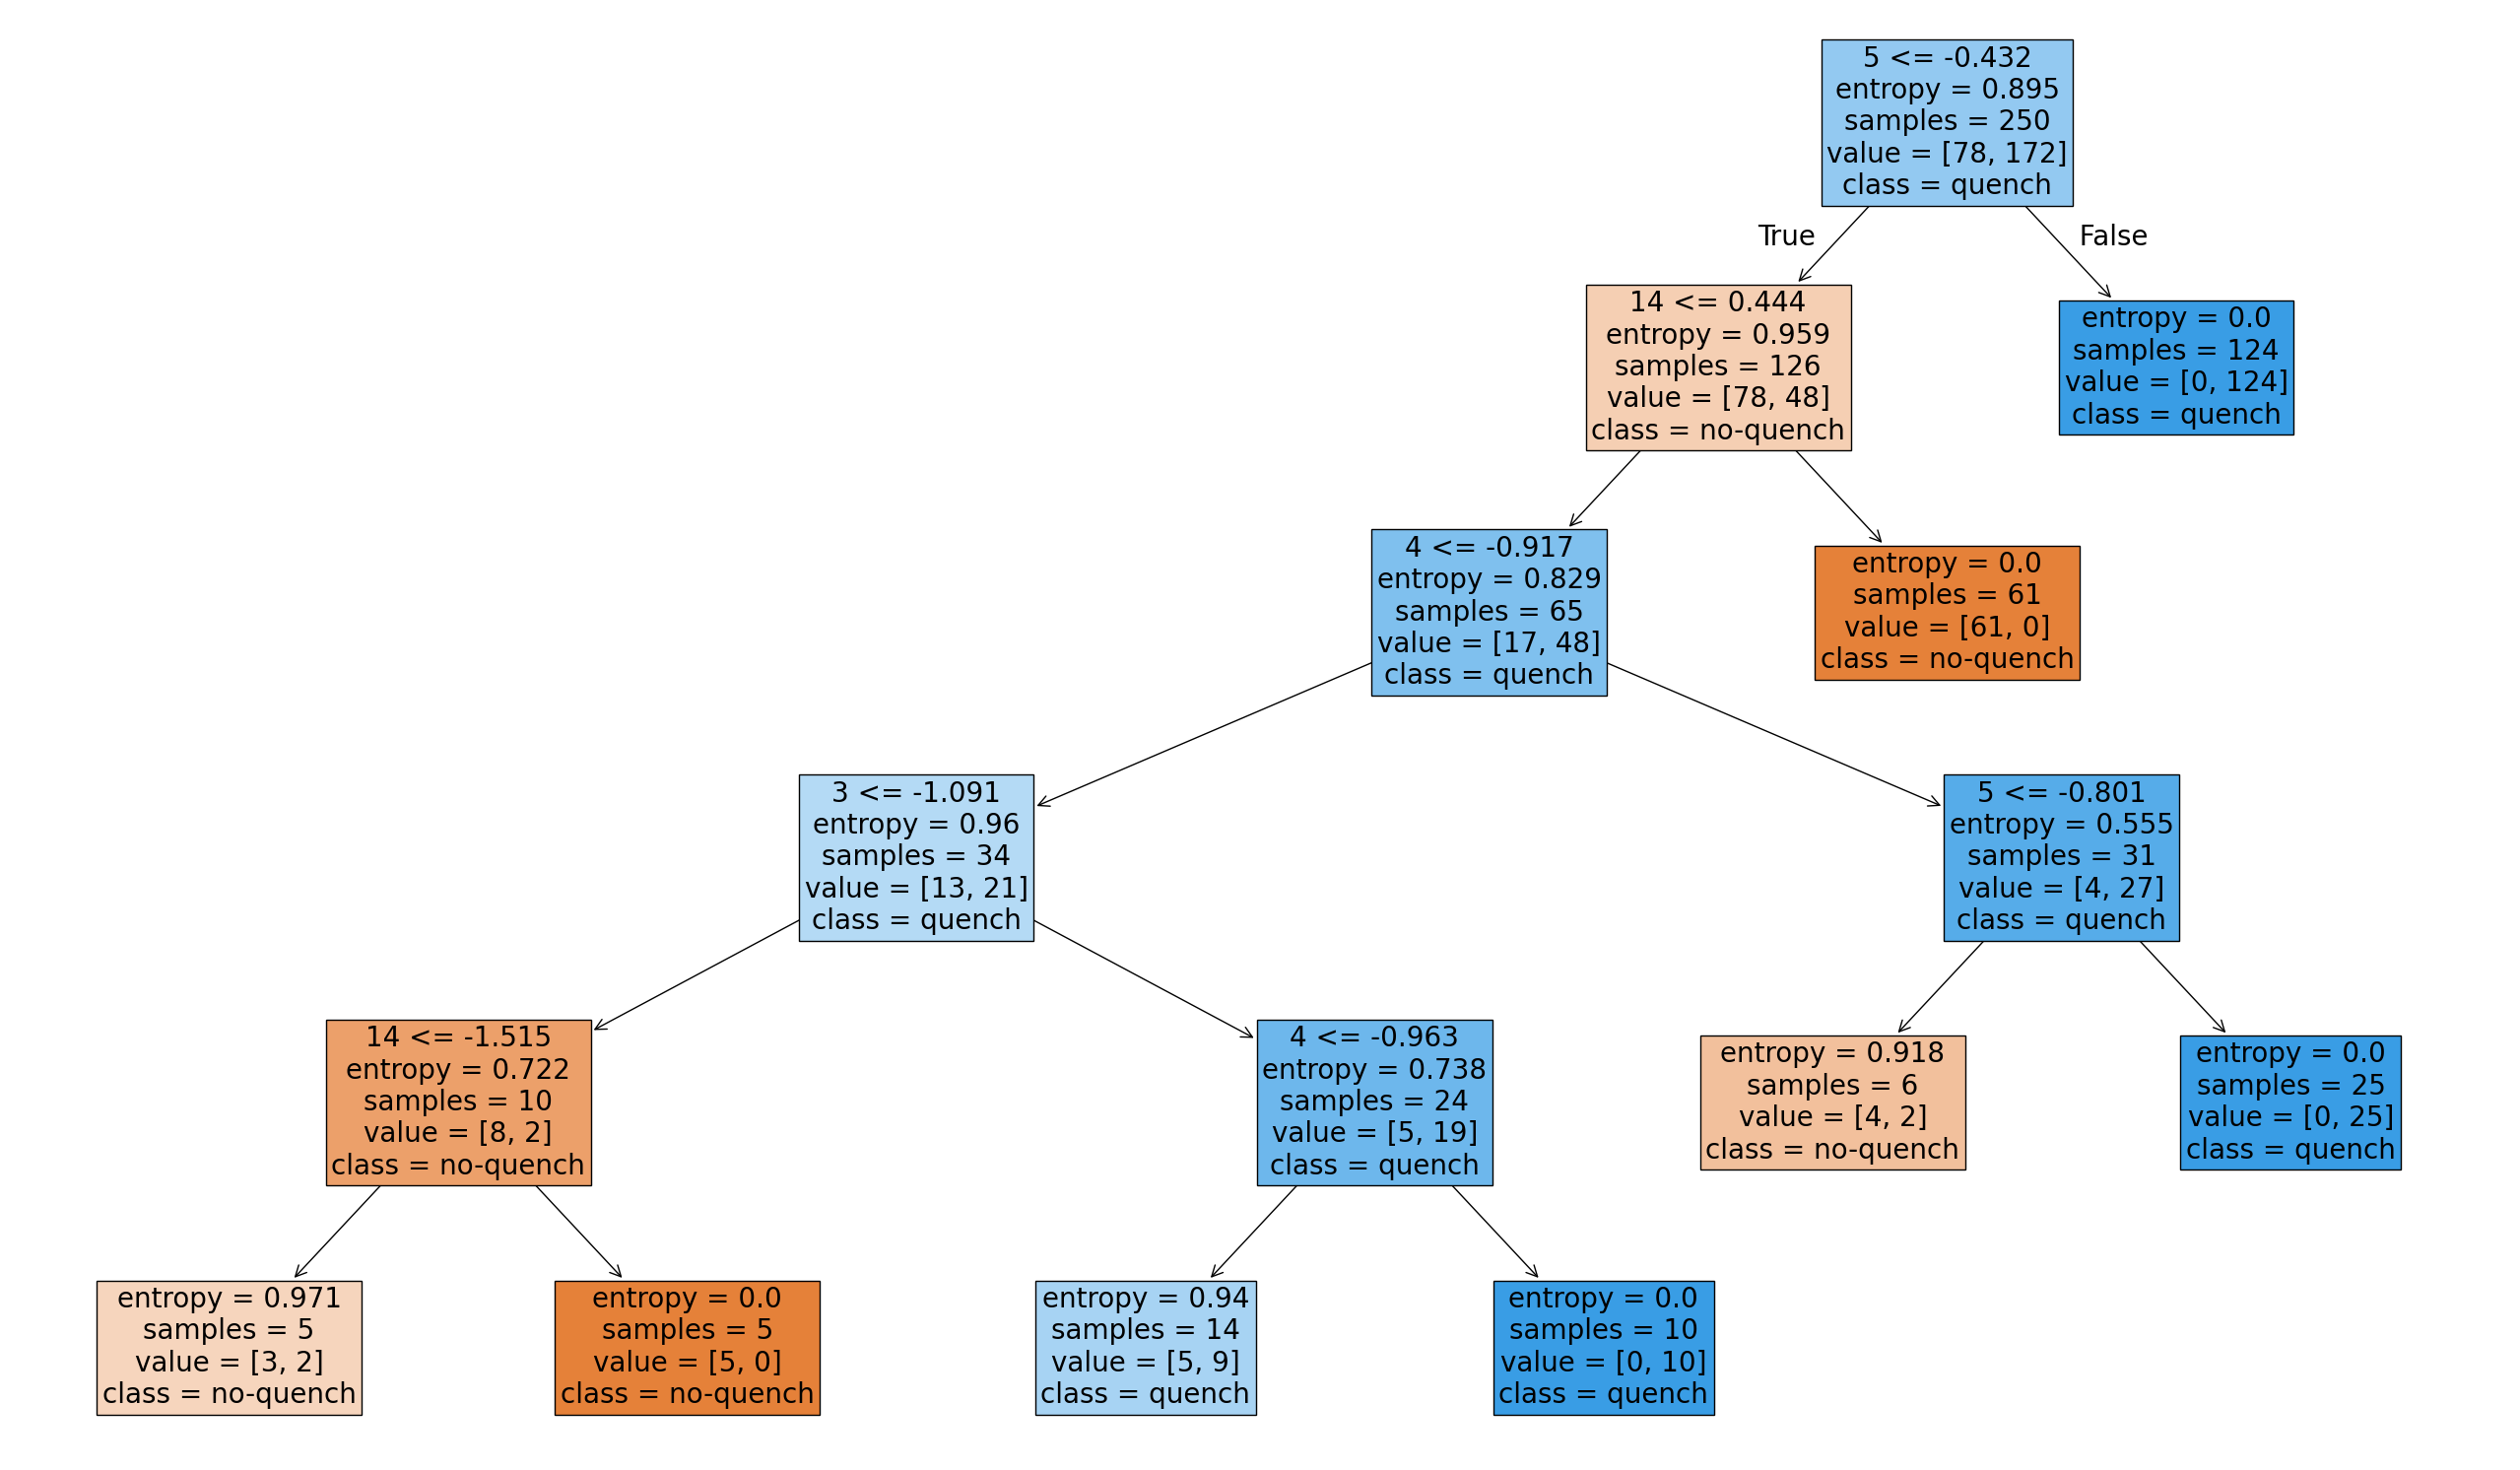
\includegraphics[width=\linewidth]{img/Cnmod_3_4_5_14_pt_dt.png}
		\subcaption{Tree trained on a subview of \cnmod}
	\end{subfigure}
	\caption{Two of the trees contained in the best \ta, the one trained on a subview of \an is
		shown in \Cref{fig:dt-an-2-12-pt}} \label{fig:part-of-bta}
\end{figure}

Finally, we evaluated the best TA on the blind test set $\mathscr D_\mathrm{test}$, obtaining only
an incorrect classification over $29$ examples (precisely, a false positive), corresponding to the
metric values detailed in Table~\ref{tab:qrp-ta-test}, essentially confirming our initial estimate.

\begin{table}[!ht]
	\caption{Performances of the best TA on the blind test set $\mathscr
			D_\mathrm{test}$.}\label{tab:qrp-ta-test}

	\bigskip
	\setlength{\tabcolsep}{6pt}
	\centering
	\begin{tabular}{cccccc}
		\toprule
		\textbf{Acc} & \textbf{Prc} & \textbf{Rec} & \textbf{F1} & \textbf{Irec} & \textbf{RAUC} \\
		\midrule
		0.965        & 0.952        & 1            & 0.976       & 0.889         & 0.944         \\
		\bottomrule
	\end{tabular}
\end{table}


\subsection{Final considerations on \qrp}
In this chapter we have introduced the problem of \qrp\ we showed many different models and we
chose the best estimator for each class (\dt, \svc, \rf, \ta). In each subsection we have
highlighted the strengths and the characteristics of the classifiers found and we provided the
results of a final blind-test; in light of all the tests that have been done...







